\documentclass{article}
\usepackage{mystyle}
\usepackage{float}
\usepackage{enumitem}
\usepackage{amsthm}
\usepackage{amsmath}
\usepackage{amssymb}
\usepackage{sgame}
\usepackage{tikz}
\usepackage{graphicx}
\usepackage[colorlinks = true, linkcolor = blue, urlcolor = cyan]{hyperref}
\usetikzlibrary{calc}

\theoremstyle{definition}
\newtheorem{theorem}{Theorem}[section]
\newtheorem{lem}{Lemma}[section]
\newtheorem{cor}{Corollary}[theorem]
\newtheorem{defn}{Definition}[section]
\newtheorem{prop}{Proposition}[section]
\newtheorem{ax}{Axiom}[section]
\newtheorem{example}{Example}[section]

\tikzset{
% Two node styles for game trees: solid and hollow
solid node/.style={circle,draw,inner sep=1.5,fill=black},
hollow node/.style={circle,draw,inner sep=1.5}
}

\title{Game Theory}
\author{
	\textbf{Raj Aryan Agrawal}\\
	190050097\\
	Undergraduate, Department of Computer Science\\
	Indian Institute of Technology Bombay
}

\begin{document}
\maketitle
\setcounter{tocdepth}{2}
\tableofcontents

\section{Introduction}
The term \textit{game} in \textit{game theory} corresponds to an interaction involving decision makers or players who are rational and intelligent. \textit{Rationality} means a player will choose a strategy to maximise his benefit while \textit{Intelligence} means the player is capable to compute his/her best strategies. It is a mathematical model that models both cooperation and competition between players/firms etc.\\

\textit{Game Theory} focuses on analysis of games and their outcomes, while \textit{Mechanism Design} focuses on designing a game so as to get required output.
\subsection{Modern Applications}
Game Theory is used in all kinds of fields ranging from Economics, Political Science, Biology, Sociology etc. Here we mention a few.
\subsubsection*{Algorithmic Game Theory and Mechanism Design}
Recent CS papers have modelled the internet as a theoretical game model and shows efficiency lost due to selfish behaviour on the internet. The system used here also led to a tool to design traffic networks and routing policies.

CS also led to start of \textit{algorithmic Mechanism Design} where MD can be used to solve algorithmic problems where inputs to the problem constitute the private information of rational and intelligent agents.
\subsubsection*{Matching Markets}
Matching is the process of allocating one set of resources or individuals to another set of resources or individuals. Like matching buyers to sellers, or doctors to hospitals. The matching has to be accomplished so that the individual preferences are honored and performance is optimized while also creating a stable matching and \textit{incentive compatible}. A solution is called incentive compatible if the preferences are reported truthfully by all the agents.
\subsubsection*{Sponsored Search}
Consider the advertisements on Google. The allocation is generally through a system where the advertisers are invited to specify their willingness to pay for specific keywords, this is the cost per click. The search engine would typically like to maximize its revenue whereas the advertisers would wish to achieve maximum payoffs within a given budget.

The search engine has to decide which advertisements to display, their order and the payments to be made by the advertiser for a click. This is a problem of designing a game for the search.
\subsubsection*{Social Network Analysis}
Social structures like business, social media, friendship etc. are visualised using Social Network Analysis. Game theoretic approaches provide a suitable approach to designing scalable algorithms for social network analysis. This is an important part of sociology.\\

In this we will be looking at some of the basic concepts behind Cooperative and Non-Cooperative Game Theory.
\subsection{Definitions}
Firstly we consider the a very common type of game - Strategic Form Games
\subsubsection{Strategic Form Games}

\begin{example}
Consider such a situation, 2 prisoners, each are kept in a separate room. Both of them are told that if they confess about the other, they will go free and the other will stay in jain for 3 years, while if both confess they each spend 2 years and if no one confesses, 1 year each. Each player independently and simultaneously chooses his option. Depending on what they choose, we can get different payoffs which can be modelled as below. This leads us to a definition.
\end{example}
\begin{figure}[H]\hspace*{\fill}%
\begin{game}{2}{2}[Player~1][Player~2]
& keep quiet & confess \\
keep quiet &$(-1,-1)$ &$(-3,0)$\\
confess &$(0,-3)$ &$(-2,-2)$
\end{game}\hspace*{\fill}%
\end{figure}
\begin{defn}
\textbf{(Strategic Form Game)} A strategic form game $\Gamma$ is a tuple $\langle N, (S_i)_{i\in\mathbb{N}},(u_i)_{i\in\mathbb{N}}\rangle$ where
\begin{itemize}
	\item $N = \{1,2\dots, n\}$ is the set of players
	\item $S_1,S_2\dots S_n$ are the strategy sets for each player
	\item $u_i:S_1\times S_2 \dots \times S_n \mapsto \mathbb{R}$ for each $i$ is the mapping of utility/payoff functions
\end{itemize}
\end{defn}
The strategies are also called actions or more specifically \textit{pure strategies} and is denoted by $S$ which is a collection of all strategy vectors.\\

We can view the play of a strategic form game as follows: each player simultaneously selects a strategy from his respective $S_i$ and informs this to a neutral observer who then computes the outcome and the utilities.
\subsubsection{Preferences}
Each player has a certain preference order for the outcomes. The preferences that a player has over outcomes can be formalized as a \textit{preference relation} over the set of outcomes {S} and this is \textit{Reflexive, Transitive} and \textit{Complete}
\subsubsection{Utilities}
The utility function or payoff function of a player is a real valued function defined on the set of all outcomes or strategy profiles. A person's utility depends not only on his strategy but on strategy of others as well. Utility Theory states that there must exist a way of assigning real numbers to different strategy profiles in a way that the decision maker would always choose the option that maximizes her expected utility.
\subsubsection{Rationality}
One of the key assumptions in game theory is that the players are rational. An agent is said to be rational if the agent always makes decisions in pursuit of her own objectives. Note that the players act out of \textit{self-interest} and do not mean to harm other players. Self interest only means each player has certain individual preferences over the outcomes and the player consistently seeks to obtain these preferred outcomes.

When such rational decision makers interact, their decision problems have to be analyzed together, like a system of simultaneous equations.
\subsubsection{Intelligence}
This notion means that each player in the game knows everything about the game that a game theorist knows, and the player is competent enough to make any inferences about the game that a game theorist can make.

An intelligent player makes his response based on expected behaviour of other players, such a response is called \textbf{Best Response Strategy}
\subsubsection{Common Knowledge}
A fact is common knowledge among the players if every player knows it, every player knows that every player knows it, and so on. 

If it happens that a fact is known to all the players, without the requirement of all players knowing that all players know it, etc., then such a fact is called \textit{mutual knowledge}. This is sort of a weaker notion of common knowledge. We can understand through an example\\

\begin{example} 
Consider an island with 100 people, all having green eyes but none of them knowing so about themselves and know about everyone else. One day an announcement is made that atleast one of them has green eyes. If a person is sure his eyes are green, he can go to the shore and escape from the island. Here we consider all players are rational and intelligent. Note that the announcement is a common knowledge. On the first 99 days nothing happens, on the 100th day all people escape the island.

This can be understood by a 2 person example, suppose A and B. A knows B has green eyes and will leave on first day if A does not have green eyes, since atleast 1 must have green eyes. B thinks the same. But on the 2nd day they see each other and realise the other must have seen another green eyed person and that is why they didnt leave. Hence both get confirmed their eyes are green.

Extending this to 3 people, from C's view, if he doesn't have green eyes, on 2nd day both A and B will leave. But he finds them on the 3rd day, that means there had to be a 3rd person as well with green eyes. Thus C is confirmed his eyes are green. Same for A and B. Same logic can be extended upwards to 100 players.
\end{example}
\subsubsection{Types of Games}
Games are represented by various forms, like a dynamic game with sequence of moves can't be represented in same way as strategic form games.
\begin{itemize}
	\item \textit{Non-cooperative Games and Cooperative Games} Non-cooperative games are those in which the actions of individual players are the primitives; in cooperative games, joint actions of groups of players are the primitives.
	\item \textit{Static Games and Dynamic Games} In a dynamic game there is a temporal order in which actions are played by the players while Static Games players choose their actions simultaneously and no information is received during the play.
	\item \textit{Games with Perfect Information and Games with Imperfect Information} When the players are fully informed about the entire past history, it is perfect information, else the latter.
	\item \textit{Complete Information and Incomplete Information Games} In a game with complete information, every aspect of the game is common knowledge. In the latter, some information may be hidden from some players at start
\end{itemize}
There are many other types like \textit{Recurring Games, Stochastic Games} etc.
\section{Dominance and Equilibrium}
\subsection{Strategic Form Games}
The idea behind the strategic form representation is that a player’s decision problem is to choose a strategy that maximises his payoff given what others are doing. Such a strategy is called a \textit{best response strategy}.
\begin{defn}
\textbf{(Best Response Strategy)} Given a strategic form game $\Gamma$ and a strategy profile $s_{-i} \in S_{-i}$ we say $s_i \in S_i$ is a Best Response Strategy wrt $s_{-i}$ iff $u_i(s_i,s_{-i} \geq u_i(s_i', s_{-i}) \forall s_i'\in S_i$ where $S_{-i} = S_1 \times \dots S_{i-1}\times S_{i+1}\times\dots S_n$
\end{defn}

\subsubsection{Competitive Game - Matching Pennies}
Both players simultaneously play. This is also called a \textit{Zero-Sum Game} where sum of payoffs is constant (taken 0 for simplicity)
\begin{figure}[H]\hspace*{\fill}%
\begin{game}{2}{2}[Player~1][Player~2]
& Head & Tail\\
Head &$(1,-1)$ &$(-1,1)$\\
Tail &$(-1,1)$ &$(1,-1)$
\end{game}\hspace*{\fill}%
\end{figure}
\subsubsection{Coordination Game - Two Drivers}
Imagine two drivers driving towards each other in a country having no traffic rules, and who must independently decide whether to drive on the left or on the right(their left/right).
\begin{figure}[H]\hspace*{\fill}%
\begin{game}{2}{2}[Player~1][Player~2]
& left & right \\
left &$(1,1)$ &$(0,0)$\\
right &$(0,0)$ &$(1,1)$
\end{game}\hspace*{\fill}%
\end{figure}
\subsubsection{Non Symmetric Game - Company Productions}
Company 1 is better known for product A and if it happens that both companies produce A, company 1 prospers. If both companies produce B, then they share the profits equally. If one of them produces A and the other produces B, then company 2 prospers.
\begin{figure}[H]\hspace*{\fill}%
\begin{game}{2}{2}[Player~1][Player~2]
& A & B \\
A &$(4,1)$ &$(0,4)$\\
B &$(1,5)$ &$(1,1)$
\end{game}\hspace*{\fill}%
\end{figure}
\subsubsection{Infinite Strategy Game - Duopoly Pricing}
There are two companies 1 and 2 which wish to maximize their profits. The demand as a function of a price $p$ is given by a continuous and strictly decreasing function $x(p)$. The cost for producing each unit of product is $c$ where $c > 0$. The companies simultaneously choose their prices $p_1$ and $p_2$. The amount sold by each company is given as
\[
  x_1(p_1,p_2) =
  \begin{cases}
  	x(p_1) & \text{if $p_1<p_2$} \\
    x(p_1)/2 & \text{if $p_1=p_2$} \\
  	0 & \text{if $p_1>p_2$}
  \end{cases}
\] and similar for other. Production costs only come for output sold, then the utility functions are $$u_1(p_1,p_2) = (p_1-c)x_1(p_1,p_2) \hspace{5mm} u_2(p_1,p_2) = (p_2-c)x_2(p_1,p_2)$$ Here $N=\{1,2\}$ and $S_1 = S_2 = [0,\infty)$. This is an infinie game since strategy sets are infinite.
\subsection{Dominant Strategies}
\begin{defn}
\textbf{((Strongly Dominated Strategy)} Given a strategic form game $\Gamma$, a strategy $s_i\in S_i$ of player $i$ is strongly dominated by another strategy $s_i'\in S_i$ if $$u_i(s_i',s_{-i})>u_i(s_i,s_{-i}) \forall s_{-i}\in S_{-i}$$
\end{defn}
\begin{defn}
\textbf{(Weakly Dominated Strategy)} Given a strategic form game $\Gamma$, a strategy $s_i\in S_i$ of player $i$ is weakly dominated by another strategy $s_i'\in S_i$ if $$u_i(s_i',s_{-i})\geq u_i(s_i,s_{-i}) \forall s_{-i}\in S_{-i} \text{ and } \exists s_{-i}\in S_{-i} \text{ s.t. } u_i(s_i',s_{-i})> u_i(s_i,s_{-i}) $$
\end{defn}
\begin{defn}
\textbf{(Very Weakly Dominated Strategy)} Given a strategic form game $\Gamma$, a strategy $s_i\in S_i$ of player $i$ is very weakly dominated by another strategy $s_i'\in S_i$ if $$u_i(s_i',s_{-i})\geq u_i(s_i,s_{-i}) \forall s_{-i}\in S_{-i}$$
\end{defn}
If a strategy (strongly/weakly/very weakly) dominates every other strategy for a player $i$, is is a (strongly/weakly/very weakly) dominant strategy.
\begin{defn}
\textbf{(Strongly(Weakly/Very Weakly) Dominant Strategy Equilibrium)} A strategy profile $s^* = (s_1^*,\dots s_n^*)$ is a strongly(weakly/very weakly) dominant equilibrium of game $\Gamma$ if $\forall i, s_i^*$ is a strongly(weakly/very weakly) dominant strategy  
\end{defn}
\subsection{Braess Paradox Game}
This is associated with transportation networks which has been applied in the real world in places like Seoul, South Korea where traffic congestion was reduced when a particular high speed link was closed for traffic. This paradox shows that a network with extra capacity may actually perform worse.
\begin{figure}[H]
\centering
\begin{minipage}[b]{0.4\textwidth}
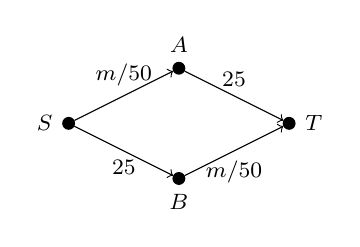
\begin{tikzpicture}[scale=0.7,font=\footnotesize]
\node[solid node,label=left:{$S$}] (S) at (-2,0){};
\node[solid node,label=above:{$A$}] (A) at (0,1){};
\node[solid node,label=below:{$B$}] (B) at (0,-1){};
\node[solid node,label=right:{$T$}] (T) at (2,0){};

\path [->] (S) edge node[above] {$m/50$} (A);
\path [->] (S) edge node[below] {$25$} (B);
\path [->] (A) edge node[above] {$25$} (T);
\path [->] (B) edge node[below] {$m/50$} (T);
\end{tikzpicture}
\caption{Transportation network}
\end{minipage}
\begin{minipage}[b]{0.4\textwidth}
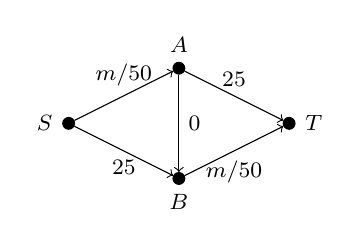
\begin{tikzpicture}[scale=0.7,font=\footnotesize]
\node[solid node,label=left:{$S$}] (S) at (-2,0){};
\node[solid node,label=above:{$A$}] (A) at (0,1){};
\node[solid node,label=below:{$B$}] (B) at (0,-1){};
\node[solid node,label=right:{$T$}] (T) at (2,0){};

\path [->] (S) edge node[above] {$m/50$} (A);
\path [->] (S) edge node[below] {$25$} (B);
\path [->] (A) edge node[above] {$25$} (T);
\path [->] (B) edge node[below] {$m/50$} (T);
\path [->] (A) edge node[right] {$0$} (B);
\end{tikzpicture}
\caption{Transportation network with extra link}
\end{minipage}
\end{figure}
Originally the situation is like left, and those are the times to travel where $m$ is the number of vehicles on that link. There are a total of 1000 vehicles. Let the people using the nodes be $n_A(s_1,\dots s_n)$ and $n_A(s_1,\dots s_n)$. Then we get 
\[
 u_i(s_1,\dots,s_n) =
 \begin{cases} -25 - \frac{n_A(s_1,\dots,s_n)}{50} & \text{ if } s_i = A \\
 \\
  -25 - \frac{n_B(s_1,\dots,s_n)}{50} & \text{ if } s_i = B
 \end{cases}
 \]
 Thus $u_i(s_1,\dots s_n) = -35$ when $n_A = n_B$. Now consider we add an extra fast link from A to B. Then we have
\[
 u_i(s_1,\dots,s_n) = 
 \begin{cases}-25 - \frac{n_A(s_1,\dots,s_n)+n_{AB}(s_1,\dots,s_n)}{50} & \text{ if } s_i = A \\
 \\
  -25 - \frac{n_B(s_1,\dots,s_n)+n_{AB}(s_1,\dots,s_n)}{50} & \text{ if } s_i = B \\
  \\
   - \frac{n_A(s_1,\dots,s_n)+n_{AB}(s_1,\dots,s_n)}{50}\\
  \hspace{5mm} - \frac{n_B(s_1,\dots,s_n)+n_{AB}(s_1,\dots,s_n)}{50} & \text{ if } s_i = AB \\
  \end{cases}
 \]
 This gives us $$u_i(AB,s_{-i}) > u_i(A,s_{-i}) \text{ and } u_i(AB,s_{-i}) > u_i(B,s_{-i}) \forall s_{-i}\in S_{-i}$$ (Note this is for the 1000 person model only). This is true for every player $i$, thus $(AB,AB\dots AB)$ is a \textit{strictly dominant straegy equilibrium}. But observe that the delay is now of $40$ minutes compared to $35$ without link. This is the paradox.
 \subsection{Iterated Elimination of Strictly Dominated Strategies}
 \begin{example}
Consider a 2 player game where each has 3 strategies to choose from,
\begin{figure}[H]\hspace*{\fill}%
\begin{game}{3}{3}[Player~1][Player~2]
& Left & Center & Right \\
Up &$(13,3)$ &$(1,4)$ &$(7,3)$\\
Middle &$(4,1)$ &$(3,3)$ &$(6,2)$\\
Down &$(-1,9)$ &$(2,8)$ &$(8,-1)$\\
\end{game}\hspace*{\fill}%
\end{figure}
Here there is no dominant strategy but we do see strictly dominated strategies.\\

Right is a strategy strictly dominated by Center, so P2 will never play Right. By rationalization, P1 knows the same, and thus now, Middle dominates the Down in such a situation ($4>-1$ and $3>2$), thus we get
\begin{figure}[H]\hspace*{\fill}%
\begin{game}{2}{2}[Player~1][Player~2]
& Left & Center\\
Up &$(13,3)$ &$(1,4)$\\
Middle &$(4,1)$ &$(3,3)$
\end{game}\hspace*{\fill}%
\end{figure}
P2 knows that P1 will deduce the dominated strategy. Continuing this, we eventualy get (Middle-Center) is the best outcome for players to play.
\end{example}
\begin{defn}
\textbf{Iterated Elimination of Strictly Dominated Strategies}
\begin{itemize}
	\item \textbf{Step 0:} Define for each $i$, $S_i^0 = S_i$
	\item \textbf{Step 1:} Define for each $i$, $$S_i^1 = \{s_i \in S_i^0 \vert \nexists s_i'\in S_i^0 \textrm{ s.t. } u_i(s_i', s_{-i}) > u_i(s_i, s_{-i}) \forall s_{-i} \in S_{-i}^0 \}$$
	\vdots
	\item \textbf{Step k:} Define for each $i$, $$S_i^k = \{s_i \in S_i^{k-1} \vert \nexists s_i'\in S_i^{k-1} \textrm{ s.t. } u_i(s_i', s_{-i}) > u_i(s_i, s_{-i}) \forall s_{-i} \in S_{-i}^{k-1} \}$$
\end{itemize}
Then the only rationable strategies to play at the end is $S_i^{\infty} = \cap_{k=0}^{\infty} S_i^k$.
\end{defn}
\section{Pure Strategy Nash Equilibrium}
A dominant strategy equilibrium requires that each player’s strategy be a best response strategy against all possible strategy choices of the other players. We get the notion of Nash equilibrium, a central notion in game theory, if we only insist that each player’s strategy offers a \textit{best response against the Nash equilibrium strategies of the other players}. This is one of the key elements to solutions of strategic games.
\begin{defn}
\textbf{(Pure Strategy Nash Equilibrium)} Given a strategic form game $\Gamma$, the strategy profile $s^* = (s_1^*,\dots, s_n^*)$ is called a PSNE of $\Gamma$ if $$u_i(s_i^*,s_{-i}^*)\geq u_i(s_i,s_{-i}^*)\forall s_i\in S_i \hspace{2mm} \forall i = 1,2\dots n$$ Or otherwie $$u_i(s_i^*,s_{-i}^*) = \max_{s_i\in S_i} u_i(s_i,s_{-i}^*) \forall i = 1,\dots n$$
\end{defn}
We can define Nash Equilibrium using best response as well
\begin{defn}
\textbf{(Best Response Correspondence)} Given a strategic form game $\Gamma$ the best response correspondence for $i$ is the map $b_i : S_{-i}\mapsto 2^{S_i}$ defined by $$b_i(s_{-i}) = \{s_i\in S_i : u_i(s_i,s_{-i})\geq u_i(s_i',s_{-i}) \forall s_i' \in S_i\}$$
\end{defn}
That is $b_i(s_{-i})$ gives the set of all best responses strategies for a given profile $s_{-i}$ for player $i$. Then a strategy profile $s^*$ is a PSNE iff $$s_i^* \in b_i(s_{-i}^*) \forall i =1,\dots n$$ That is every players strategy is a best respone to others' strategies.
\subsection{Bandwidth Sharing Game}
There is a shared communication channel of maximum capacity 1. There are $n$ users of this channel, and user $i$ wishes to send $x_i$ units of flow, where $x_i \in[0,1]$. If $\sum_{i\in N} x_i \geq 1$ then the transmission can't happen, if $<1$ the payoff is $$u_i(x_1,x_2\dots x_n) = x_i(1 - \sum_{j \in N} x_j) \forall i\in N$$ Let us define $t_i = \sum_{j\neq i}x_j$ For maximising payoff, i.e. best strategy $$x_i^* = arg\max_{x_i\in[0,1]} x_i(1-t_i-x_i) = \frac{1-t_i}{2} \forall i = 1,2,\dots n$$
For a Nash Equilibrium, every player is playing his/her best strategy. So $t_i = \sum_{j \neq i} x_j^*$. Thus we get n equations in n variables. On solving we get $$x_i^* = \frac{1}{n+1} \forall i = 1,2\dots n$$ This is a PSNE and the payoff for each player is $$u_i = \frac{1}{(n+1)^2}$$ Although the profile $(1/2n,1/2n \dots 1/2n)$ is an optimal solution, such a situation is not stable, hence not a NE.
\subsection{Procurement Exchange Exam}
Suppose that there are two sellers, 1 and 2, and three buyers A, B, and C. Suppose the constraints are
\begin{itemize}
	\item A can only buy from seller 1
	\item C can only buy from seller 2
	\item B can buy from either seller 1 or seller 2
	\item Each buyer has maximum willingness of 1 to pay
	\item Sellers have enough items to sell
	\item Each seller announces a price in $[0,1]$
\end{itemize}
Let $s_1$ and $s_2$ be the prices and suppose B will buy from seller 1 if $s_1 = s_2$, then the game is
\begin{align*}
u_1(s_1,s_2) &= 2s_1 \text{ if } s_1\leq s_2 & u_2(s_1,s_2) &= 2s_2 \text { if } s_1>s_2\\
&= s_1 \text{ if } s_1>s_2 &&= s_2 \text{ if } s_1\leq s_2
\end{align*}
First observe that $u_2(1,s_2)$ has value $2s_2$ for $s_2\in [0,1)$ and suddenly drops to 1 at $s_2 = 1$, thus such a strategy can't be a NE for any $s_2$. Now consider $u_1(s_1,1)$, the best response here is $s_1 = 1$ but we saw above that $s_1 = 1$ cannot give a NE, so we get for NE, $s_1, s_2 \in [0,1)$

\textbf{Case 1:} If $s_1^* \leq 1/2$, best response of player 2 is $s_2 = 1$ but this can't be a NE.

\textbf{Case 2:} If $s_1^* > 1/2$ then either $s_1^* \leq s_2^*$ or $s_1^* > s_2^*$. Consider former, then $u_1 = 2s_1^*$ and $u_2 = s_2^*$. Player 2 can choose $s_2$ s.t $1/2<s_2<s_1^*$, then $u_2(s_1^*, s_2) = 2s_2 > s_2^* = u_2(s_1^*, s_2^*)$. Hence this is not a NE.\\

Now consider latter, $u_1 = s_1^*$ and $u_2 = 2s_2^*$. Consider $s_1$ s.t. $1>s_1>s_1^*$, then $u_1(s_1, s_2^*) = s_1 > s_1^* = u_1(s_1^*, s_2^*)$ Thus not a NE. \textit{This game has no Pure Strategy Nash Equilibrium}
\subsection{Interpretation of Nash Equilibrium}
By deviating from a Nash equilibrium strategy, a player will not be better off given that the other players do not deviate from their Nash equilibrium strategies. Some interpretations are
\begin{itemize}
	\item It can be viewed as an advice to each player for strategy to play. Note that this is only against one player deviating, multiple players deviating can give a better payoff - Prisoner's Dilemmma.
	\item Another view is \textit{Prediction}. If all players are rational and intelligent, a reduction of dominated strategies will give a reduced form that includes a Nash Equilibrium.
	\item Another interpretation is \textit{Self-Enforcing Agreement} as once the agreement is reached, its in personal benefit of each player to remain true to it.
	\item It's also viewed as \textit{evolution and steady state}. As the playes observe behaviour of others and adjust, they converge to the equilibrium position.
	\item The conjectures of the players are consistent: each player $i$ chooses $s_i^*$ expecting all other players to choose $s_{-i}^*$, and each player’s conjecture is verified in a Nash equilibrium.
\end{itemize}
\subsection{Multiple Nash Equilibria - Schelling Focal Point}
If there are multiple Nash Equilibria, we can't make a unique prediction. An important idea here is \textit{Schelling's Focal Point}. According to Schelling, anything that tends to focus the players' attention on one equilibrium may make them all expect it and fulfill it.\\

\begin{example} 
Ask the people to meet in New York, without specifying the place. Most people will go to Grand Central. Meeting at Grand Central, as opposed to meeting at any one of thousands of similar places, is a \textit{focal point}
\end{example}
\subsection{Maxmin Value and Minmax Value}
If a player wants to play so as to protect her payoff against any possible irrationality of the other players, then she has to plan for a worst case situation. Such situations lead to maxmin strategies.
\subsubsection{Maxmin Value and Maxmin Strategy}
The notion of a maxmin strategy of a player looks at the best possible payoff the player can guarantee herself even in the worst case when the other players are free to choose any strategies.
\begin{defn}
\textbf{(Maxmin Value and Maxmin Strategy)} Given a strategic form game $\Gamma$, the maxmin value of a player $i$ is given by $$\underline{v_i}= \max_{s_i\in S_i} \min_{s_{-i} \in S_{-i}} u_i(s_i, s_{-i})$$ Any strategy $s_i^*\in S_i$ that guarantees this payoff is called \textit{maxmin strategy}.
\end{defn}
That is, this is the maximum of his minimum payoffs.\\
\begin{example} 
Consider game
\begin{figure}[H]\hspace*{\fill}%
\begin{game}{2}{2}[Player~1][Player~2]
& A & B\\
A &$(4,1)$ &$(0,4)$\\
B &$(1,5)$ &$(1,1)$
\end{game}\hspace*{\fill}%
\end{figure}
If player 1 plays A, his minimum payoff would be 0, while if he played B it would be 1. Thus 1 is his maxmin value and B is the maxmin strategy.
\end{example}
\begin{prop}
Suppose a strategic form game $\Gamma$ has a Pure Strategy Nash Equilibrium then $$ u_i(s_1^*\dots s_n^*) \geq \underline{v_i} \hspace{3mm}\forall i\in N$$
\end{prop}
\begin{proof}
Firstly $$u_i(s_1^*, \dots s_n^*) = \max_{s_i \in S_i} u_i(s_i,s_{-i}^*)$$ And obviously $\forall i \in N$ $$u_i(s_i,s_{-i}^*) \geq \min_{s_{-i}\in S_{-i}} u_i(s_i,s_{-i})$$
Combining the 2 we get $u_i(s_1^*, \dots s_n^*) \geq \underline{v_i} \hspace{2mm} \forall i \in N$
\end{proof}
A profile of maxmin strategies is another solution concept for a strategic form game.
\subsubsection{Minmax Value}
When all other players choose strategies that hurt player $i$ the most, the minimum value that can be forced on player $i$ is \textit{minmax value}. That is, this is the minimum of all his maximum payoffs.
\begin{defn}
\textbf{(Minmax Value and Minmax Strategy)} Given a strategic form game $\Gamma$ the minmax value of a player $i$ is given by $$\bar{v_i} = \min_{s_{-i}\in S_{-i}} \max_{s_i\in S_i} u_i(s_i, s_{-i})$$ Any strategy profile $s_{-i}^*\in S_{-i}$ of other player that forces the payoff $\bar{v_i}$ is called a minmax strategu profile (for rest of the players)
\end{defn}
\begin{example}
In the game above, if P1 plays A the maximum P2 could get is 4, while if he played B the maximum P2 could get is 5. So the minmax value of P2 is 4 and the strategy for P1 against P2 is strategy A
\end{example}
Now, since minmax is the maximum payoff player $i$ can get when all players try their best to hurt him, and maxmin is the minimum payoff the player can guarantee himself of recieving, naturally minmax value is greater.
\begin{prop}
\label{Minmax greater}
Consider a strategic form game $\Gamma$, then $$\bar{v_i} > \underline{v_i} \forall i \in N$$
\end{prop}
\begin{proof}
Suppose $s_{-i}^*$ is the minmax strategy, then $$\bar{v_i} \geq \max_{s_i\in S_i} u_i(s_i, s_{-i}^*) \forall i\in N$$ And also $$u_i(s_i,s_{-i}^*) \geq \min_{s_{-i}\in S_{-i}} u_i(s_i,s_{-i}) \forall s_i\in S_i$$ Combining we get $$\bar{v_i} \geq \max_{s_i\in S_i} \min_{s_{-i} \in S_{-i}} u_i(s_i, s_{-i}) = \underline{v_i} \forall i \in N$$
\end{proof}
\begin{prop}
Suppose a strategic form game $\Gamma$ has a pure strategy nash equilibrium, then $$u_i(s_1^*,\dots s_n^*) \geq \bar{v_i}\hspace{2mm} \forall i \in N$$
\end{prop}
\begin{proof}
Consider the Nash Strategy profile is $(s_1^* \dots s_n^*)$. Note that $$\max_{s_i\in S_i} u_i(s_i, s_{-i}^*) \geq \min_{s_{-i}\in S_{-i}} \max_{s_i\in S_i} u_i(s_i, s_{-i})\forall i \in N$$ The left side is the definition of Nash Equilibrium $$u_i(s_1^*,\dots s_n^*) \geq \bar{v_i}\hspace{2mm} \forall i \in N$$
\end{proof}
\subsection{Minimax Regret}
Consider the other players are unpredictable(like in MaxMin). In such a setting, it can also make sense for agents to care about minimizing their worst-case loss, rather than simply maximizing their worst-case payoff. This is regret.\\
\begin{example} 
Consider game 
\begin{figure}[H]\hspace*{\fill}%
\begin{game}{2}{2}[Player~1][Player~2]
& L & R\\
T &$(100,a)$ &$(1-\epsilon,b)$\\
B &$(2,c)$ &$(1,d)$
\end{game}\hspace*{\fill}%
\end{figure}
P1 can think so, if player 2 were to play R then the maximum he can lose is $\epsilon$ which is not much, instead if P2 plays L, P1's choice can greatly change his payoff. Thus P1 can play T to reduce his worst-case loss
\end{example}
\begin{defn}
\textbf{(Regret)} A player's regret for playing strategy $s_i$ if others play profile $s_{-i}$ is defined as $$\left[ \max_{s_i'\in S_i} u_i(s_i',s_{-i})\right] - u_i(s_i,s_{-i})$$
\end{defn}
This is the loss amount by not playing his best response.
\begin{defn}
\textbf{(Max Regret)} A player's max regret is defined as $$\max_{s_{-i}\in S_{-i}}\left(\left[ \max_{s_i'\in S_i} u_i(s_i',s_{-i})\right] - u_i(s_i,s_{-i})\right)$$
\end{defn}
This is the loss by not playing his best response when every other player is trying to maximise the loss.
\begin{defn}
\textbf{(Minimax Regret)} Minimax regret strategies for player $i$ is defined as
$$arg \min_{s_i\in S_i} \left[\max_{s_{-i}\in S_{-i}}\left(\left[ \max_{s_i'\in S_i} u_i(s_i',s_{-i})\right] - u_i(s_i,s_{-i})\right)\right]$$
\end{defn}
This is the action that gives the smallest maximum regret. Minimax regret can be extended to a solution concept in the natural way, by identifying strategy profiles that consist of minimax regret actions for each player.
\section{Extensive Form Games}
Extensive form games with a finite number of players and with a finite number of actions available to each player are depicted graphically using game trees.\\
\subsection{Definition}
\begin{example}
\textbf{(Matching Pennies with Observation)}
Consider 2 players, both play H or T, if both coins show same side, player 1 takes the money, else player 2. The game tree consists of $(1)$ Root node (initial decision) $(2)$ Internal nodes (decision nodes) and $(3)$ Leaves (outcome nodes). Each path is called a \textit{Path of Play}.
\end{example} 
\begin{figure}[H]\hspace*{\fill}%
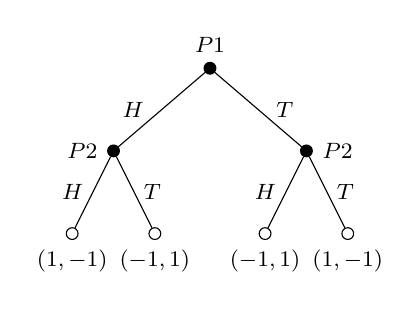
\begin{tikzpicture}[scale=0.7,font=\footnotesize]
\centering
% Specify spacing for each level of the tree
\tikzstyle{level 1}=[level distance=15mm,sibling distance=35mm]
\tikzstyle{level 2}=[level distance=15mm,sibling distance=15mm]
% The Tree
\node(0)[solid node,label=above:{$P1$}]{}
child{node(1)[solid node, label=left:{$P2$}]{}
child{node[hollow node,label=below:{$(1,-1)$}]{} edge from parent node[left]{$H$}}
child{node[hollow node,label=below:{$(-1,1)$}]{} edge from parent node[right]{$T$}}
edge from parent node[left,xshift=-3]{$H$}
}
child{node(2)[solid node,label=right:{$P2$}]{}
child{node[hollow node,label=below:{$(-1,1)$}]{} edge from parent node[left]{$H$}}
child{node[hollow node,label=below:{$(1,-1)$}]{} edge from parent node[right]{$T$}}
edge from parent node[right,xshift=3]{$T$}
};
\end{tikzpicture}\hspace*{\fill}%
\caption{Game Tree with Player1 starting}
\end{figure}
\begin{example}
\textbf{(Matching Pennies without Observation)} The other player does not observe the outcome and only puts down her rupee coin heads up or tails up. The set of connected nodes (by dotted lines) is called \textit{information set} in which player doesn't know the node in information set.
\end{example}
\begin{figure}[H]\hspace*{\fill}%
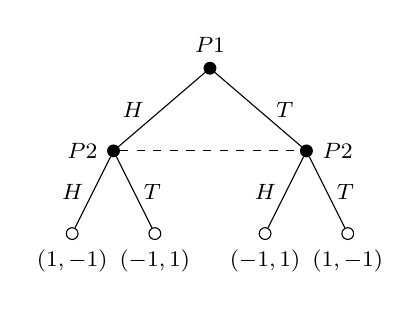
\begin{tikzpicture}[scale=0.7,font=\footnotesize]
\centering
% Specify spacing for each level of the tree
\tikzstyle{level 1}=[level distance=15mm,sibling distance=35mm]
\tikzstyle{level 2}=[level distance=15mm,sibling distance=15mm]
% The Tree
\node(0)[solid node,label=above:{$P1$}]{}
child{node(1)[solid node, label=left:{$P2$}]{}
child{node[hollow node,label=below:{$(1,-1)$}]{} edge from parent node[left]{$H$}}
child{node[hollow node,label=below:{$(-1,1)$}]{} edge from parent node[right]{$T$}}
edge from parent node[left,xshift=-3]{$H$}
}
child{node(2)[solid node,label=right:{$P2$}]{}
child{node[hollow node,label=below:{$(-1,1)$}]{} edge from parent node[left]{$H$}}
child{node[hollow node,label=below:{$(1,-1)$}]{} edge from parent node[right]{$T$}}
edge from parent node[right,xshift=3]{$T$}
};
% information set
\draw[dashed](1)to(2);
\end{tikzpicture}\hspace*{\fill}%
\caption{Game Tree with Player1 starting}
\end{figure}
\begin{example}
\textbf{(Matching Pennies with Simultaneous Play)} This is the same as previous scenario, since both players dont know about each other and make thier decision.
\end{example}
\begin{defn}
\textbf{(Information Set)} An information set of a player is a set of that player’s decision nodes that are indistinguishable to her. 
\end{defn}
So, in the 2nd example, we have $\{\varepsilon\}$ as the only information set for 1 and $\{H,T\}$ for 2nd.
\begin{defn}
\textbf{(Extensive Form Game)} An extensive form game $\Gamma$ consists of tuple

$\langle N, (A_i)_{i\in\mathbb{N}}, \mathbb{H}, P, (\mathbb{I}_i)_{i\in\mathbb{N}}, (u_i)_{i\in\mathbb{N}}\rangle$ where
\begin{itemize}
	\item $N=\{1,2,\dots,n\}$ is a finite set of players
	\item $A_i$ for all $i$ is the set of all actions availble to player $i$
	\item $\mathbb{H}$ is the set of all terminal histories where a terminal history is a path of actions from the root to a terminal node such that it is not a proper subhistory of any other terminal history. $S_{\mathbb{H}}$ denotes the set of all proper subhistories
	\item $P: S_{\mathbb{H}} \mapsto N$ is a function that associates each subhistory to a player
	\item $\mathbb{I}_i$ is the set of all information sets for player $i$
	\item $u_i : \mathbb{H} \mapsto R$ for each $i$ gives utility of each player corresponding to history
\end{itemize}
\end{defn}
For example, for first example we have $\mathbb{H} = \{(H,H),(H,T),(T,H),(T,T)\}, S_{\mathbb{H}} = \{\varepsilon, H, T\}, P(\varepsilon) = 1, P(H) = 2, \mathbb{I}_2 = \{\{H\},\{T\}\}$
\begin{defn}
\textbf{(Perfect Information and Imperfect Information Games)} An extensive form game with perfect information is one in which all the information sets are singletons. Else it is imperfect information.
\end{defn}
\begin{theorem}
Every finite perfect information game in extensive form has a pure strategy nash equilibrium
\end{theorem}
\begin{proof}
The proof is direct since at each instance every player can choose optimal moves based and there is no need to introduce randomness.
\end{proof}
\subsection{Transforming Extensive Form to Strategic Form}
A strategy can be described as a complete action plan that specifies what a player will do at each of the information sets where he is called upon to play.
\begin{defn}
\textbf{(Strategy)} A strategy $s_i$ of player $i$ is a mapping $s_i : \mathbb{I}_i \mapsto A_i$ such that $s_i(J) \in C(J)\forall J\in \mathbb{I}_i$ where $C(J) \subseteq A_i$ be the set of all actions possible to player $i$ in information set $J$
\end{defn}
A strategy determines the action the player will choose in every stage or history of the game the player is called upon to play.
\begin{example}
\textbf{(Matching Pennies with Observations)} We have $\mathbb{I}_1 = \{\{\varepsilon\}\} \mathbb{I}_2 = \{\{H\},\{T\}\}$. Player 1 has 2 strategies $$s_{11}:\{\varepsilon\} \mapsto H \hspace{5mm} s_{12}:\{\varepsilon\} \mapsto T$$ and Player 2 has 4 $$s_{21}:\{H\} \mapsto H \hspace{2mm} \{T\} \mapsto H \hspace{5mm} s_{22}:\{H\} \mapsto H \hspace{2mm} \{T\} \mapsto T$$ $$s_{23}:\{H\} \mapsto T \hspace{2mm} \{T\} \mapsto H \hspace{5mm} s_{24}:\{H\} \mapsto T \hspace{2mm} \{T\} \mapsto T$$ Then the strategic form will be as below
\end{example}
\begin{figure}[H]\hspace*{\fill}%
\begin{game}{2}{4}[Player~1][Player~2]
& $s_{21}$ & $s_{22}$ & $s_{23}$ & $s_{24}$ \\
$s_{11}$ &$(1,-1)$ &$(1,-1)$ &$(-1,1)$ &$(-1,1)$\\
$s_{12}$ &$(-1,1)$ &$(1,-1)$ &$(-1,1)$ &$(1,-1)$
\end{game}\hspace*{\fill}%
\end{figure}
Note that a strategy profile uniquely determines a terminal history since each strategy profile gives a path of play.
\begin{defn}
\textbf{(Outcome)} Given an extensive form game $\Gamma$ and a strategy profile $s = (s_1,\dots,s_n)$ in the game, the outcome resulting out of the terminal history corresponding to the strategy profile $s$ is called the outcome of $s$ and is denoted by $O(s)$.
\end{defn}
\begin{defn}
\textbf{(Consistent Strategy)} Let $x=(a_1,\dots,a_k)$ be a node by the given path (a subhistory). A pure strategy $s_i$ is consistent with $x$ if for each segment of path $(a_1,\dots,a_l)$ with $l<k$ and $P(a_1,\dots,a_l)=i$ then $s_i(a_1,\dots,a_l) = a_{l+1}$. That is player $i$ chooses actions as denoted by $x$
\end{defn}
However, the strategic form representation suppresses the dynamics of the game because of simultaneous play. Games where the order and dynamics matter are generally solved in extensive form.
\subsection{Equilibria in Extensive Form Games}
\begin{defn}
\textbf{(Subgame)} Given an extensive form game $\Gamma$ and a non terminal history $h$ the subgame following $h$ is the part of the game that remains after history $h$ has occured.
\end{defn}
Basically it's the remaining possible game after a certain sequence of actions have taken place.
\subsubsection{Pure Strategy Nash Equilibrium}
The notion is direct once we represent an extensive form game as strategic form.
\begin{defn}
\textbf{(Pure Strategy Nash Equilibrium for Extensive Form Games)} Given an extensive form game $\Gamma$, a strategy profile $s^* = (s_1^*, \dots s_n^*)$ is a pure strategy nash equilibrium if $\forall i\in N$
$$u_i(O(s_i^*, s_{-i}^*))\geq u_i(O(s_i, s_{-i}^*)) \forall s_i \in S_i$$ where $O(.)$ denotes outcome of a strategic profile.
\end{defn}
\begin{example}
\textbf{(The Entry Game)}
Consider the game 
\begin{figure}[H]\hspace*{\fill}%
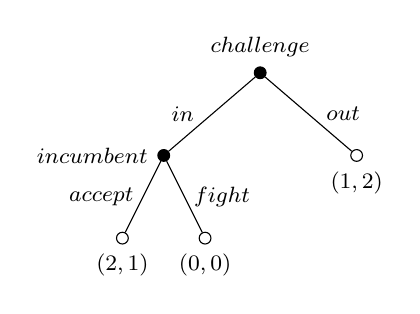
\begin{tikzpicture}[scale=0.7,font=\footnotesize]
\centering
% Specify spacing for each level of the tree
\tikzstyle{level 1}=[level distance=15mm,sibling distance=35mm]
\tikzstyle{level 2}=[level distance=15mm,sibling distance=15mm]
% The Tree
\node(0)[solid node,label=above:{$challenge$}]{}
child{node(1)[solid node, label=left:{$incumbent$}]{}
child{node[hollow node,label=below:{$(2,1)$}]{} edge from parent node[left]{$accept$}}
child{node[hollow node,label=below:{$(0,0)$}]{} edge from parent node[right]{$fight$}}
edge from parent node[left,xshift=-3]{$in$}
}
child{node(2)[hollow node,label=below:{$(1,2)$}]{}
edge from parent node[right,xshift=3]{$out$}};
\end{tikzpicture}\hspace*{\fill}%
\end{figure}
(challenger) either decides to challenge the incumbent (action: in) or drops out (action: out). Player 2 (incumbent) either decides to fight or accommodate the challenger in case the challenger decides to confront the incumbent. This can be converted to strategic form game as
\begin{figure}[H]\hspace*{\fill}%
\begin{game}{2}{2}[Player~1][Player~2]
& accept & fight\\
in &$(2,1)$ &$(0,0)$\\
out &$(1,2)$ &$(1,2)$
\end{game}\hspace*{\fill}%
\end{figure}
It is clear that $(in,accept)$ and $(out,fight)$ are both pure strategy nash equilibrium. But the 2nd doesnt make much sense since player 2 never got the chance to choose. Such a scenario is explained using \textit{threat} where P2 threats to fight. However, such a threat is \textit{non credible threat}. Thus we need a better notion for equilibrium.
\end{example}
\subsection{Subgame Perfect Equilibrium}
It requires each player’s strategy to be \textit{optimal} not only at the start of the game, but also after every history.
\begin{defn}
\textbf{(Subgame Perfect Equilibrium)} Given an extensive form game $\Gamma$, a strategy profile $s^*$ is an SGPE if $\forall i\in N$
$$u_i(O_h(s_i^*, s_{-i}^*))\geq u_i(O_h(s_i, s_{-i}^*)) \hspace{2mm}\forall h\in\{x\in S_\mathbb{H}:P(x) = i\} \hspace{4mm} \forall s_i\in S_i$$ where $O_h(s_i^*, s_{-i}^*)$ is the outcome corresponding to history h in the strategy profile $(s_i^*, s_{-i}^*)$
\end{defn}
Thus the profile should be an equilibrium for every subgame as well. From SGPE, we see $(out, fight)$ is not an SGPE as \textit{fight} is not optimal if first chooses \textit{in}. SGPE are computed using \textit{Backward Induction}
\subsection{Backward Induction}
Backward induction refers to starting from the last subgames of a finite game, then finding the best response strategy profiles or the Nash equilibria in the subgames, then assigning these strategies profiles and the associated payoffs to be subgames, and moving successively towards the beginning of the game. For a 2 player zero sum game, this is called the \textit{minimax algorithm}
\begin{prop}
Backward Induction gives the entire set of SGPE.
\end{prop}
\begin{proof}
Backward induction makes sure that in the restriction of the strategy profile in question to any subgame is a Nash equilibrium.
\end{proof}
\begin{prop}
Every finite perfect information extensive form game $\Gamma$ has a pure strategy SGPE
\end{prop}
\begin{proof}
Start from the end by backward induction and at each step atleast one strategy is best response. Since we have perfect information, we never have to guess between which moves the opponent has played.
\end{proof}
\begin{example} 
Consider 5 pirates who found a treasure chest of 100 gold coins. The 5 pirates are A,B,C,D,E with that order of authority. First A will propose a distribution, if equal or more agree, they will distribute, otherwise A is killed and B is the captain and so on. We need the equilibrium distribution\\

This an extensive form game, so let us consider the last subgame, where only D and E are remaining, then D proposes 100 coins to him and 0 to E. So E will not want this. This is an equilibrium for this subgame. Now consider the higher subgame, C,D and E. If C gives 1 coin to E, E will support C as it increases his payoff, and D gets 0. So D will not want this. Continuing up, we find the equilibrium strategy for A is $(98,0,1,0,1)$ distribution.
\end{example}
\subsection{One-Stage Deviation Principle}
This is basically the principle of optimality used in Dynamic Programming.
\begin{theorem}
For a finite horizon extensive game with perfect information, $s^*$ is a SGPE iff $\forall i,t,h^t$ $$u_i(O_{h^t}(s_i^*, s_{-i}^*))\geq u_i(O_{h^t}(s_i, s_{-i}^*))$$ for all $s_i$ satisfying $s_i(h^t) \neq s_i^*(h^t)$ and $s_{i\vert h^t}(h^{t+k}) = s_{i\vert h^t}^*(h^{t+k}) \forall k>0$ and $\forall h^{t+k} \in \Gamma(h^t)$ where $h^t$ is a given non terminal history upto t levels and $s(h^t)$ is a possible strategy at level $t$ and $s_{\vert h}$ is the restricted strategy given $h$ happened.
\end{theorem}
That is, s is an SGPE iff no player $i$ can gain by deviating from $s$ in a single stage and conforming to $s$ thereafter. The proof of one-stage deviation principle for finite horizon games relies on the idea that if a strategy satisfies the one stage deviation principle then that strategy cannot be improved upon by a finite number of deviations. Thus we need some term for infinite games
\subsection{Infinite Horizon Games}
\begin{defn}
Consider an infinite moves game, $\Gamma^{\infty}$ and let $h\in \mathbb{H}$ be an $\infty$-horizon history and let $h^t$ be its restriction to first $t$ moves(levels). The game is \textbf{continuous at infinity} if $\forall i\in N$, 
$$ \sup_{h,h' s.t. h^t = h'^t} \vert u_i(h) - u_i(h') \vert \mapsto 0 \text{ as } t \mapsto \infty$$
\end{defn}
The continuity at infinity condition is satisfied when the overall payoffs are a discounted sum of stage payoffs, i.e. $$u_i = \sum_{t=1}^{\infty}\delta_i^t g_i^t(s^t)$$ where $s^t$ is the set of strategies at stage $t$, $g_i^t(s^t)$ is the stage payoff and $\delta<1$ is the discount factor and the stage payoff functions are uniformly bounded, that is, $\exists B\in \mathbb{R}$ s.t. $\max_{t,s^t} \vert g_i^t(s^t) \vert < B$
\begin{theorem}
For an infinite horizon infinite extensive game that is continuous at infinity with perfect information, $s^*$ is a SGPE iff $\forall i,t,h^t$ $$u_i(O_{h^t}(s_i^*, s_{-i}^*))\geq u_i(O_{h^t}(s_i, s_{-i}^*))$$ for all $s_i$ satisfying $s_i(h^t) \neq s_i^*(h^t)$ and $s_{i\vert h^t}(h^{t+k}) = s_{i\vert h^t}^*(h^{t+k}) \forall k>0$ and $\forall h^{t+k} \in \Gamma(h^t)$
\end{theorem}
This can be thought of same as finite strategy, and since continuous, the deviations decrease as we go down, so even an infinite deviations will not affect.
\subsection{Value of Commitment}
Suppose we exchange the timing of decisions in the entry game (i.e. Player2 - Incumbent) chooses accept or fight first, then $(fight, out)$ is the SPE (before this was discared, this time the other is). This is the \textit{value of commitment} (where P2 commits to fight)
\section{Mixed Strategies and Mixed Strategy Nash Equilibrium}
A natural generalization of pure strategies leads to mixed strategies. A mixed strategy of a player associates a probability distribution over the pure strategies of the player. We assume $S_i$ is finite for each $i$.
\begin{defn}
\textbf{(Mixed Strategy)} Given a player $i$ with $S_i$ as the set of pure strategies, a mixed strategy $\sigma_i$ is a probability distribution over $S_i$.
\end{defn}
A pure strategy is just a mixed strategy with $s_i =1$ and rest $0$. The set $\Delta (S_i)$ is the set of all probability distributions over set $S_i$. This is the \textit{mixed extension} of $S_i$. $$\Gamma_{ME} = \langle N, (\Delta(S_i)), (U_i) \rangle$$ where $U_i$ is mapping that maps mixed strategy profile to $\mathbb{R}$, i.e. $U_i: \times_i \Delta(S_i) \mapsto \mathbb{R}$. Note that we will generally use $u_i$ instead. Considering that the randomization of each player is independant, $\sigma(s_1,\dots s_n) = \Pi_{i\in N} \sigma_i(s_i)$ and the payoff is $$U_i(\sigma_1, \dots \sigma_n) = \sum_{(s_1,\dots,s_n)\in S} \sigma(s_1,\dots,s_n) u_i(s_1,\dots,s_n)$$
We can directly convert Nash Equilibrium and best response to Mixed Strategy version by replacing $s_i, s_{-i}, S_i$ with $\sigma_i, \sigma_{-i}, \Delta(S_i)$. Thus a mixed strategy profile is a Nash Equilibrium iff $\sigma_i^* \in b_i(\sigma_{-i}^*) \forall i\in N$
\subsection{Interpretations of Mixed Strategy}
\begin{itemize}
	\item Mixed strategy are a description of what might happen in repeated play, the count of pure strategies in the limit.
	\item Mixed strategies describe population dynamics. Suppose we have a population of Player1's and another of Player2's. 2 players are randomly chosen from the population, both having deterministic strategies, then the mixed strategy gives probability of getting each pure strategy. Example - \href{https://www.youtube.com/watch?v=YNMkADpvO4w&t=7s}{Primer example of Red and Blue blobs}
\end{itemize}
\subsection{Properties of Mixed Strategies}
\begin{defn}
\textbf{(Convex Combination)} Given real numbers $y_1, \dots, y_n$ a convex combination is a weighted sum $\lambda_1y_1 +\dots + \lambda_ny_n$ where $0\leq\lambda_i\leq1 \forall i = 1\dots n$ and $\sum_{i=1}^n \lambda_i = 1$
\end{defn}
\begin{prop}
\label{convex}
Let $\Gamma$ be a strategic form game. Then $u_i(\sigma_i,\sigma_{-i})$ can be expressed as the convex combination $$u_i(\sigma_i,\sigma_{-i}) = \sum_{s_i \in S_i} \sigma_i(s_i)u_i(s_i, \sigma_{-i})$$ where $$u_i(s_i, \sigma_{-i}) = \sum_{s_{-i}\in S_{-i}}\left(\prod_{j\neq i}\sigma_j(s_j)\right)u_i(s_i,s_{-i})$$
\end{prop}
\begin{proof}
\begin{align*}
u_i(\sigma_i,\sigma_{-i}) & = \sum_{s\in S} \left(\prod_{j\in N}\sigma_j(s_j)\right) u_i(s_i,s_{-i})\\
& = \sum_{s_i\in S_i} \sum_{s_{-i}\in S_{-i}} \left(\prod_{j\neq i}\sigma_j(s_j)\right)\sigma_i(s_i) u_i(s_i, s_{-i})\\
& = \sum_{s_i \in S_i} \sigma_i(s_i)\left\{ \sum_{s_{-i}\in S_{-i}}\left(\prod_{j\neq i}\sigma_j(s_j)\right)u_i(s_i,s_{-i})\right\}
\end{align*}
Which gives $u_i(\sigma_i,\sigma_{-i}) = \sum_{s_i \in S_i} \sigma_i(s_i)u_i(s_i, \sigma_{-i})$
\end{proof}
\begin{prop}
\label{maximum}
Given a strategic form game $\Gamma$, then for any $\sigma \in \times_{i\in N} \Delta(S_i)$ and for any player $i$ $$\max_{\sigma_i\in \Delta(S_i)} u_i(\sigma_i, \sigma_{-i}) = \max_{s_i \in S_i} u_i(u_i, \sigma_{-i})$$ Also, $$\rho_i \in arg \max_{\sigma_i \in \Delta(S_i)}u_i(\sigma_i,\sigma_{-i}) \iff \rho_i(x) = 0 \forall x\notin arg \max_{s_i\in S_i} u_i(s_i,\sigma_{-i})$$
\end{prop}
\begin{proof}
We can express it as a convex combination as $$u_i(\sigma_i,\sigma_{-i}) = \sum_{s_i \in S_i} \sigma_i(s_i)u_i(s_i, \sigma_{-i})$$ The maximum of convex combination is simply the maximum of the values. So $$\max_{\sigma_i\in \Delta(S_i)} u_i(\sigma_i, \sigma_{-i}) = \max_{s_i \in S_i} u_i(u_i, \sigma_{-i})$$ A mixed strategy $\rho_i$ will attain maximum value iff $$\sum_{x\in X} \rho_i(x) = 1 \text{ where } X = arg \max_{s_i\in S_i} u_i(s_i, \sigma_{-i})$$ Which is equivilent to the given statement.
\end{proof}
The second part basically says, to get maximum value, the only strategies which contribute are the ones that give maximum value.
\subsection{Condition for Profile to be a Nash Equilibrium}
We now prove a condition which helps us in evaluating mixed strategy nash equilibriums.
\begin{defn}
\textbf{(Support of a Mixed Strategy)} Let $\sigma_i$ be any mixed strategy for player $i$, the support is denoted by $\delta(\sigma_i)$ which is the set $$\delta(\sigma_i) = \{s_i\in S_i:\sigma_i(s_i)>0\}$$That is these strategies have non zero contribution in mixed strategy.
\end{defn}
\begin{defn}
\textbf{(Support of a Profile)} Let $\sigma$ be a mixed strategy profile with $\delta(\sigma_i)$ as the support for $\sigma_i$ then the support $\delta(\sigma)$ of profile $\sigma$ is $\times_i \delta(\sigma_i)$
\end{defn}
\begin{theorem}
\label{conditions}
The mixed strategy profile $(\sigma_1^*, \dots, \sigma_n^*)$ is a mixed strategy nash equilibrium iff $\forall i\in N$,

$(1) u_i(s_i, \sigma_{-i}^*)$ is the same $\forall s_i\in\delta(\sigma_i^*)$ and 

$(2) u_i(s_i, \sigma_{-i}^*) \geq u_i(s_i', \sigma_{-i}^*)$
\end{theorem}
\begin{proof}
\textbf{Necessity:} $\sigma^*$ is a profile for nash equilibrium, thus $$u_i(\sigma_i^*, \sigma_{-i}^*)\geq u_i(\sigma_i, \sigma_{-i}^*) \forall \sigma_i \in \Delta(S_i)$$ So, we get $$u_i(\sigma_i^*, \sigma_{-i}^*) = \max_{\sigma_i\in \Delta(S_i)} u_i(\sigma_i, \sigma_{-i}^*) = \max_{s_i\in S_i}u_i(s_i, \sigma_{-i}^*)$$ using Proposition \ref{maximum} and thus $$\sum_{s_i \in S_i} \sigma_i^*(s_i)u_i(s_i,\sigma_i^*) = \max_{s_i\in S_i}u_i(s_i, \sigma_{-i}^*)$$ using \ref{convex} and since $\sigma_i^*(s_i) = 0 \forall s_i\notin \delta(\sigma_i)$, $$\sum_{s_i \in \delta(\sigma_i^*)} \sigma_i^*(s_i)u_i(s_i,\sigma_i^*) = \max_{s_i\in S_i}u_i(s_i, \sigma_{-i}^*)$$ Consider a convex combination $\lambda_1x_1 +\dots \lambda_nx_n$ with $\lambda_i \neq 0 \forall i = 1, \dots,n$ such that $\sum \lambda_i =1$ and $\sum \lambda_ix_i = \max(x_1, \dots, x_n)$ then $x_1 = x_2 = \dots = x_n = \max(x_1, \dots, x_n)$ Using this we get $$u_i(s_i, \sigma_{-i}^*) = \max_{s_i\in S_i}u_i(s_i, \sigma_{-i}^*)= u_i(\sigma_i^*, \sigma_{-i}^*) \forall s_i \in \delta(\sigma_i^*) \forall i \in N$$ This also directly gives $(2)$\\

\textbf{Sufficiency:} We are given that $u_i(s_i,\sigma_{-i}^*$ has same value, suppose $w_i$ for all $s_i\in \delta(\sigma_i^*)$ and $u_i(s_i,\sigma_{-i}^* \geq u_i(s_i',\sigma_{-i}^* \forall s_i \in \delta(\sigma_i^*)$ and $\forall s_i' \notin \delta(\sigma_i^*)$. Then we need to prove $u(\sigma^*)$ is a nash equilibrium.
\begin{align*}
u_i(\sigma_i^*, \sigma_{-i}^*) &= \sum_{s_i \in S_i} \sigma_i^*(s_i)u_i(s_i,\sigma_{-i}^*)  = \sum_{s_i \in \delta_i(\sigma_i^*)} \sigma_i^*(s_i)u_i(s_i,\sigma_{-i}^*)\\
&= \sum_{s_i \in \delta_i(\sigma_i^*)} \sigma_i^*(s_i) w_i = w_i &\text{ (Condition 1)}\\
&= \sum_{s_i\in S_i} \sigma_i(s_i)w_i \forall \sigma_i\in \Delta(S_i) \geq \sum_{s_i \in S_i} \sigma_i(s_i)u_i(s_i,\sigma_{-i}^*) &\text{ (Condition 2)}\\
&- u_i(\sigma_i, \sigma_{-i}^*)
\end{align*}
Hence $\sigma^*$ is a mixed strategy nash equilibrium.
\end{proof}
\subsection{Implications of The Conditions}
\begin{itemize}
	\item Given a mixed nash, each player gets same payoff by playing any pure strategy from equilibrium profile support.
	\item The above implies that the player can be indifferent about the pure strategies (but playing a pure strategy will change best responses for others)\\

	 If Player1 makes such a mixed strategy that Player2 becomes indifferent then it doesn’t matter what Player2 chooses, so if Player2 also chooses a mixed strategy such that Player1 becomes indifferent, so he is satisfied with his strategy and so is Player2, thus getting a MSNE.
	\item To verify a profile, it is enough to consider the effects of only pure strategy deviations
	\item To identify pure strategy equilibrium, it is enough to look at pure strategy game, that is, if it is an equilibrium there, it will remain in mixed extension of game. Below is the proof.
\end{itemize}
\begin{prop}
Let $e(s_i)$ be the degenerate mixed strategy that assigns $1$ to $s_i$ and $0$ to rest. A strategy profile $s^*$ is a pure strategy nash equilibrium of game $\Gamma$ iff the mixed strategy profile $e(s_1^*),\dots ,e(s_n^*)$ is a mixed strategy nash equilibrium for $\Gamma_{ME}$
\end{prop}
\begin{proof}
\textbf{Sufficiency:} Let $e(s_1^*),\dots ,e(s_n^*)$ be a mixed strategy nash, this
\begin{align*}
&\implies u_i(e(s_i^*), e(s_{-i}^*))\geq u_i(\sigma_i,e(s_{-i}^*)) \forall \sigma_i \in \Delta(S_i)\\
&\implies u_i(s_i^*, s_{-i}^*)\geq u_i(\sigma_i,s_{-i}^*) \forall \sigma_i \in \Delta(S_i)\\
&\implies u_i(s_i^*, s_{-i}^*)\geq u_i(e(s_i),s_{-i}^*) \forall s_i \in S_i\\
&\implies u_i(s_i^*, s_{-i}^*)\geq u_i(s_i,s_{-i}^*) \forall s_i \in S_i
\end{align*}
Thus $s^*$ is a pure strategy nash equilibrium.

\textbf{Necessity:} Given $s^*$ is pure nash
\begin{align*}
&\implies u_i(s_i^*, s_{-i}^*)\geq u_i(s_i,s_{-i}^*) \forall s_i \in S_i\\
&\implies u_i(e(s_i^*), e(s_{-i}^*))\geq u_i(s_i,e(s_{-i}^*)) \forall s_i \in S_i\\
&\implies u_i(e(s_i^*), e(s_{-i}^*)) = \max_{s_i \in S_i} u_i(s_i,e(s_{-i}^*)) \forall s_i \in S_i\\
&\implies u_i(e(s_i^*), e(s_{-i}^*)) = \max_{\sigma_i \in \Delta(S_i)} u_i(\sigma_i,e(s_{-i}^*)) & \text{Proposition } \ref{maximum}\\
&\implies u_i(e(s_i^*), e(s_{-i}^*)) \geq u_i(\sigma_i,e(s_{-i}^*))\forall \sigma_i \in \Delta(S_i)
\end{align*}
Thus $e(s_1^*),\dots ,e(s_n^*)$ is a mixed nash equilibrium
\end{proof}
\textbf{Note:} The definitions of Maxmin, Minmax and Dominance are the exact same as their pure counterparts by replacing $s_i, s_{-i}$ etc. with their mixed counterparts. And in Iterated Elimination of Strictly Dominated Strategies, we can change the condition that a strategy can be eliminated if even a mixed strategy strictly dominates it.
\subsection{Unsymmetric Matching Pennies}
Consider a variant of matching pennies game like
\begin{figure}[H]\hspace*{\fill}%
\begin{game}{2}{2}[Player~1][Player~2]
& A & B\\
A &$(3,-3)$ &$(-2,2)$\\
B &$(-1,1)$ &$(0,0)$
\end{game}\hspace*{\fill}%
\end{figure}
We can see there is no pure strategy Nash Equilibrium. Also, we can check all supports except $\{A,B\}\times \{A,B\}$ do not lead to any Nash Equilibrium. We now check for the mentioned one. Here condition $(2)$ is trivially satisfied, since support is the entire strategy set, so we need to check condition $(1)$ $$u_1(A,\sigma_2^*)= u_1(B,\sigma_2^*) \hspace{5mm} u_2(\sigma_1^*, A)= u_2(\sigma_1^*,B)$$ Taking $\sigma_1^* = (x,1-x)$ and $\sigma_2^* = (y,1-y)$ we get $(\sigma_1^* = (1/6,5/6), \sigma_2^* = (1/3,2/3))$ is a Nash Equilibrium.
\subsection{Mixed Strategies in Infinite Games}
For countably finite games, we define mixed strategy in almost the same way, $\sigma_i$ is a probability distribution over $S_i$, only condition is that the support $\delta(\sigma_i)$ should be \textbf{finite}.\\

For uncountably infinite strategy sets $S_i$, we define our mixed strategy in terms of \textit{probability density}. Consider a mixed strategy density function profile $\sigma$ in $S$, then the expected utility is $$u_i(\sigma) = \int_S u_i(s)d\sigma(s)$$
\subsection{Rationalizability}
In the Nash equilibrium concept, each player’s action is optimal conditional on the belief that the other players also play their Nash equilibrium strategies. Now, we consider a different solution concept in which a player's belief is not assumed to be correct but simply constrained by rationality.\\
A \textbf{belief} of a player $i$ is the response of his opponents $\sigma_{-i}$. In rationality, players maximise wrt some beliefs about opponents (i.e. they are rational) and every player is aware of other players being rational and being aware of their rationality and so on.\\

A rational deduction can look like "“I am playing strategy $\sigma_1$ because I think player 2 is using $\sigma_2$, which is a reasonable belief because I would play it if I were player 2 and I thought player 1 was using $\sigma_1'$, which is a reasonable thing to expect for player 2 because $\sigma_1'$ is a best response to $\sigma_2'$ \dots".\\
A rational player will never play a strategy that will never be a best response for any strategy used by opponents. 
\begin{defn}
\textbf{(Never Best Response)} A pure strategy $s_i$ is a never-best response if for all beliefs $\sigma_{-i},~\exists \sigma_i\in \Delta(S_i)$ such that $$u_i(\sigma_i,\sigma_{-i})>u_i(s_i,\sigma_{-i})$$
\end{defn}
Note that every strictly dominated strategy is a never best response, but the converse is not true. A never best response may not be strictly dominated by all other strategies, but this implies, for any $\sigma_{-i}$ there is some other strategy that will give better payoff (not all strategies may do better for a given $\sigma_{-i}$ like in strictly dominated).\\
By iterated elimination, we can get set $R_i^{\infty}$ which is the set of all rationalizable strategies for player $i$. Also let $D_i^\infty$ be the set of strategies that survive iterated strict dominance and $NE_i$ denote the set of pure strategies that have a positive probability in any mixed Nash Equilibrium,then $$NE_i\subseteq R_i^\infty \subseteq D_i^\infty$$
Rationalizability is more important in correlated scenarios (which we will check in cooperative games)
\subsection{Imperfect Information Extensive Form Games}
We had looked at solution to games using SGPE where every player knew the actions performed by others and where they lie in the game, but as in the example of matching pennies without observation, it was not a perfect information.\\

Imperfect information games can be of 2 types, \textit{perfect recall} and \textit{imperfect recall}. 
\begin{defn}
\textbf{(Perfect Recall)} Player $i$ has perfect recall for an extensive form game $\Gamma$ if for any 2 decision nodes $h$ and $h'$ in the same information set for player $i$, any path $h_0,a_0,h_1,\dots,h_n,a_n,h$ from root to game $h$ (where $h_j$ are decision nodes and $a_j$ are the actions), and $h_0,a_0',h_1',\dots,h_m',a_m',h'$ be the path to node $h'$, then
\begin{itemize}
	\item $n = m$ (that is they must be on the same level, player knows which stage is going on)
	\item $\forall 0\leq j\leq n$, $h_j$ and $h_j'$ belong to the same equivalence class (i.e. the class representing a possible choice for player) for player $i$
	\item $\forall 0\leq j\leq n$, if $P(h_j)=i$ then $a_j = a_j'$ (player $i$ makes same decision)
\end{itemize}
A game has perfect recall if every player has perfect recall in it. 
\end{defn}
In simple terms, in perfect recall no player forgets any information he knew about moves made so far and remembers all his moves. With introduction of perfect recall, we need notion of a term behavioural strategies.
\begin{defn}
\textbf{(Behavioral Strategies)} In these strategies, instead of having a mixed strategy over multiple fixed pathways, each player makes a choice for action independently of choices at other nodes so far.
\end{defn}
The use of this will be explained in the example,\\
\begin{example}
\begin{figure}[H]\hspace*{\fill}%
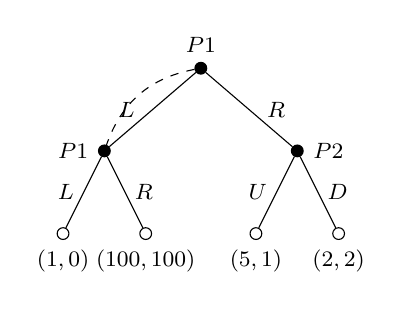
\begin{tikzpicture}[scale=0.7,font=\footnotesize]
\centering
% Specify spacing for each level of the tree
\tikzstyle{level 1}=[level distance=15mm,sibling distance=35mm]
\tikzstyle{level 2}=[level distance=15mm,sibling distance=15mm]
% The Tree
\node(0)[solid node,label=above:{$P1$}]{}
child{node(1)[solid node, label=left:{$P1$}]{}
child{node[hollow node,label=below:{$(1,0)$}]{} edge from parent node[left]{$L$}}
child{node[hollow node,label=below:{$(100,100)$}]{} edge from parent node[right]{$R$}}
edge from parent node[left,xshift=-3]{$L$}
}
child{node(2)[solid node,label=right:{$P2$}]{}
child{node[hollow node,label=below:{$(5,1)$}]{} edge from parent node[left]{$U$}}
child{node[hollow node,label=below:{$(2,2)$}]{} edge from parent node[right]{$D$}}
edge from parent node[right,xshift=3]{$R$}
};
% information set
\draw[dashed, bend right](0)to(1);
\end{tikzpicture}\hspace*{\fill}%
\caption{Game with imperfect recall}
\end{figure}
If we consider only the mixed strategies and not behavioral, the pure strategies for player 1 is $L$and $R$ (there is only 1 information set, due to imperfect recall). And player2 only has $U$ and $D$.\\
On playinh $L$, the payoff is $(1,0)$ (in both turns he will play $L$, since the strategy is same - the flaw of mixed strategies), so $R$ strictly dominates $L$, and $D$ is the best response, so $(R,D)$ is the unique Nash Equilibrium.\\
Now consider instead P1 played a behavioral strategy where he keeps a probability of each action set in an information set. Suppose he uses behavioral strategy $(p,1-p)$, the expected payoff is $$u_1 = 1*p^2 + 100*p(1-p) + 2*(1-p)$$ (as D is still player 2's best response). The utility is maximum at $98/198$, thus $(\sigma_1^* = (98/198,100/198),\sigma_2^*=(0,1))$ is the new equilibrium.
\end{example}
Note that in imperfect information games also we can use Backward induction, the only constraint is that a subgame can't slice an information set (entire information set should be retained or removed).\\
We will now prove that actually for games with perfect recall, mixed and behavioral strategies are equivalent, before that we need to define a few terms. Consider a mixed strategy $\sigma_i$ for player $i$, then the probability of player $i$ chooses a pure stratey consistent with a Subhistory $x$ is $$\pi_i(x) = \sum \sigma_i(s_i)$$ where summation is across $s_i$ consistent with $x$. Then the probability the Subhistory $x$ is followed is $\prod_{i\in N} \pi_i(x)$
\begin{theorem}
\textbf{(Kuhn's Theorem)} In a game of perfect recall, any mixed strategy can be replaced by an equivalent behavioral strategy, and any behavioral strategy can be replaced by an equivalent mixed strategy. Here two strategies are equivalent in the sense that they induce the same probabilities on outcomes, for any fixed strategy profile (mixed or behavioral) of the remaining players.
\end{theorem}
\begin{proof}
The proof is constructive. Consider we have a behavioral strategy $b_i$, we assign to a pure strategy) $s_i$, the probability $$\sigma(s_i) = \prod_{J\in \mathbb{I}_i} b_i(J)(s_i(J))$$ with the product taken over all information sets of player $i$ where the term being multiplied is basically, for infomation set $J$, the probability of action being $s_i(J)$.\\
Now consider we are given a mixed strategy $\sigma_i$. Consider an information set $J\in\mathbb{I}_i$ and a feasible action $a\in C(J)$ where $C(J)$ is set of all actions available to player $i$ in information set $J$. Now consider a node $x\in J$. Firstly note that for a game of perfect recall, $\pi(x) = \pi(y) \forall x,y\in J$ where $J$ is an information set.Then $$b_i(J)(a) = \frac{\pi_i(x,a)}{\pi_i(x)} \text{ if } \pi_i(x)>0\text{ arbitrary otherwise}$$ That is, if $x$ is consistent so far, how likely is it to choose action $a$ (Note, we need perfect recall, as if $\pi_i(x) \neq \pi_i(y)$ the probability distribution in behavioral stragies might not sum up to 1)
\end{proof}
We will not be discussing these topics and equilibrium concepts for these games.
\section{Utility Theory}
Utilities play a central role in game theory. They capture the preferences that the players have for different outcomes in terms of real numbers thus enabling real valued functions to be used in game theoretic analysis. The question arises whether it is possible at all to capture all the preferences without losing any information. Utility theory deals with this problem in a systematic and scientific way. We will study \textit{von Neumann and Morgensterm}.
\subsection{Ordinal Utilities}
Let $\succeq_i$ represent the preferance relation of player $i$, we are interested in a utility function $u_i$ such that $$x_1 \succeq_i x_2 \iff u_i(x_1)\geq u_2(x_2)$$
A scale on which larger numbers represent more preferred outcomes in a way that only the order of the numbers matters and not their absolute or relative magnitude is called an \textit{ordinal scale} and utility numbers determined in this way are \textit{ordinal utilities}.\\

\begin{example} 
Consider a game with 2 players 1 and 2 and 4 outcomes $X = \{x,y,z,w\}$. Suppose player 1 has preference order $x\succ y\succ z\succ w$ and player 2 be the opposite $w\succ z\succ y\succ x$. If we need to assign real numbers to those outcome to reflect preference ordering, there are infinite ways. One such can be $$Player~1: x:4;y:3;z:2;w:1 \hspace{5mm} Player~2: x:2;y:4;z:6;w:9$$
The numerical values here only capture order of preference, for degree of preference we use something called \textit{Preferences over Lotteries}.
\end{example}

To describe the interaction of preferences when there is uncertainty about which outcome will be selected, the notion of a lottery (or probability distribution) is a natural tool that can be used. Suppose $X= \{x_1,\dots x_m\}$, then a lottery on $X$ is a probability distribution $$\sigma = [p_1:x_1; p_2:x_2;\dots p_m:x_m]$$ and $p_j\geq 0$ and $\sum_{j=1}^m p_j = 1$. We need to understand how do different lotteries compare, that is, which lottery will a person choose.
\subsection{Axioms of von Neumann - Morgenstern Utility Theory}
We efine the preferences as binary relations as 
\begin{itemize}
	\item $x_1 \succeq x_2$: outcome $x_1$ weakly preffered over $x_2$
	\item $x_1 \succ x_2$: outcome $x_1$ strictly preffered over $x_2$
	\item $x_1\sim x_2$: both outcomes equally preffered
\end{itemize}
This directly gives
\begin{itemize}
	\item $x_1\succ x_2 \iff x_1 \succeq x_2$ and $\neg(x_2 \succeq x_1)$
	\item $x_1 \sim x_2 \iff x_1 \succeq x_2$ and $x_2 \succeq x_1$
\end{itemize}
To extend the binary relations to the set of lotteries to capture preferences over lotteries, we consider 6 axioms and prove through that.
\begin{ax}
\textbf{(Completeness)}\\

The completeness property means every pair of outcome is relaed by prefereance relation. Also the preference relation $\succeq$ induces an ordering, i.e. $$x_1\succ x_2 \text{ or } x_2 \succ x_1 \text{ or } x_1 \sim x_2 \forall x_1,x_2 \in X$$
\end{ax}
\begin{ax}
\textbf{(Transitivity)}\\
$$x_1\succeq x_2 \text{ and } x_2\succeq x_3 \implies x_1\succeq x_3 \forall x_1,x_2,x_3 \in X$$
\end{ax}
\begin{ax}
\textbf{(Substitutability)}\\

This is also called as \textit{independence}. If $x_1\sim x_2$ then for all sequences of one or more outcomes $x_3, \dots x_m$ and sets of probabilities $p, p_3,\dots p_m$ such that $$p+\sum_{j=3}^m p_j = 1$$ the player is indifferent to lotteries $\sigma_1 = [p:x_1; p_3:x_3; \dots p_m:x_m]$ and $\sigma_2 = [p:x_2; p_3:x_3; \dots p_m:x_m]$. We write this as $\sigma_1 \sim \sigma_2$
\end{ax}
In such a setting we can always replace $x_1$ with $x_2$
\begin{ax}
\textbf{(Decomposibility)}\\

This is also called \textit{simplification of lotteries}. Let $P_{\sigma}(x_i)$ denote probability that $x_i$ is selected by $\sigma$ then the axiom states that $$P_{\sigma_1}(x_i) = P_{\sigma_2}(x_i) \forall x_i \in X\implies \sigma_1 \sim \sigma_2 \forall \sigma_1,\sigma_2 \in \Delta(X)$$
\end{ax}
For example, $\sigma_1 = [0.6:x_1; 0.4:[0.4:x_1; 0.6:x_2]] \sim \sigma_2 = [0.76:x_1;0.24:x_2]$. Thus we can simplify a compound lottery to a simple lottery.
\begin{ax}
\textbf{(Monotonocity)}\\

Consider a player who strictly prefers $x_1$ to $x_2$, and $\sigma_1, \sigma_2$ are 2 lotteries over $\{x_1,x_2\}$ then monotonicity means player prefers lottery that assigns higher probability to $x_1$, that is
$$x_1\succ x_2 \text{ and } 1\geq p>q\geq 0 \implies [p:x_1;1-p:x_2] \succ [q:x_1;1-q:x_2]$$
\end{ax} 
\begin{ax}
\textbf{(Continuity)}\\
$$x_1\succ  x_2 \text{ and } x_2\succ x_3 \implies \exists p\in[0,1] \text{ s.t. } x_2 \sim [p:x_1;1-p:x_3]$$ 
\end{ax}
\begin{lem}
Suppose a relation $\succeq$ satisfies \textit{completeness, transitivity, decomposibility} and \textit{monotonicity} satisfies $x_1\succ x_2$ and $x_2 \succ x_3$ then $\exists p\in [0,1]$ s.t. $$x_2\succ [q:x_1;1-q:x_3]\hspace{2mm} \forall 0\leq q<p$$ $$[r:x_1;1-r:x_3]\succ x_2  \hspace{2mm}\forall 1\geq r>p$$
\end{lem}
\begin{proof}
Let us call $[p:x_1;1-p:x_3]$ as $\delta(p)$ Consider a probability $p_l$ such that $x_2 \succ \delta(p_l)$. Such a $p_l$ exists as $x_2\succ x_3$. And by transitivity $x_1\succ x_3$, so by monotonocity $$\delta(p_l) \succ \delta(p') \forall 0\leq p'<p_l$$ Thus by transitivity $$x_2 \succ \delta(p') \forall 0\leq p'\leq p_l$$
Similarly consider a $p_h$ such that $\delta(p_h)\succ x_2$ and such a $p_h$ exists as $x_1\succ x_2$. Thus by same arguments as above we get $$\delta(p')\succ x_2 \forall 1\geq p'\geq p_h$$
Now left is the interval $(p_l, p_h)$. Now consider $p^* = (p_l+p_h)/2$, then by completeness, we have 3 possibilities - 
\begin{itemize}
	\item $x_2 \sim \delta(p^*)$
	\item $x_2 \succ \delta(p^*)$
	\item $\delta(p^*) \succ x_2$
\end{itemize}
If the first is true, firstly there can't be any $p' \neq p^*$ such that $x_2 \sim \delta(p')$ as that gives $[\delta(p^*) \sim \delta(p')$ but that violates monotonocity ($x_1\succ x_3$). Thus for all $p' \neq p^*$, we have $x_2 \succ \delta(p')$ or $\delta(p') \succ x_2$.

Next, we can't have any $p' > p^*$ such that $x_2 \succ \delta(p')$ as by monotonicity we get $x_2 \succ \delta(p^*)$ which is contradictory. So for all $1\geq p' >p^*$ we have $\delta(p') \succ x_2$. Similarly, we get for all $0\leq p' < p^*$,we get $ x_2 \succ \delta(p')$. Thus we proved for this case\\

Next, consider $x_2 \succ \delta(p^*)$, then by monotonicity, $x_2 \succ \delta(p')\forall 0\leq p'\leq p^*$. We can re-define our $p_l = p^*$ and repeat. Similarly if $\delta(p^*) \succ x_2$, we replace $p_h = p^*$. Evenetually we will encounter $p^*$ such that $x_2\sim \delta(p^*)$ or in the limit $p_l$ and $p_h$ approach the same $p$ from both sides.  
\end{proof}
\subsection{The von Neumann - Morgenstern Theorem}
\begin{theorem}
Given a set of outcomes $X = \{x_1,\dots x_m\}$ and a preferance relation $\succ$ on $X$ that satisfies the 6 axioms, there exists a utility function $u:X\mapsto [0,1]$ with the following properties
\begin{enumerate}
	\item $u(x_1)\geq u(x_2) \iff x_1\succeq x_2 \forall x_1, x_2 in X$
	\item $u([p_1:x_1;p_2:x_2;\dots p_m:x_m]) = \sum_{j=1}^m p_j u(x_j)$
\end{enumerate}
\end{theorem}
\begin{proof}
First, consider the degenerate case $x_i \sim x_j \forall x_i,x_j \in X$. Consider function $u(x_i) = 0 \forall x_i \in X$. Part 1 is direct by definition. For part2 $u([p_1:x_1;p_2:x_2;\dots p_m:x_m]) = u([p_1:x_1;p_2:x_1;\dots p_m:x_1])$ by substitutability, which gives $u([\sum p_i: x_1]) = u(x_1) = 0$ by decomposability. RHS is $0$ as $u(x_i) = 0 \forall x_i \in X$ Hence part2 is true.\\

Now consider it is not degenerate, then by completeness, there exists atleast one most preffered outcome and atleast 1 least preffered with them being different outcomes. Let these be $\bar{x}$ and $\underline{x}$. Clearly $\bar{x}\succ \underline{x}$. Now by continuity, for any $x_i \in X \exists p_i$ such that $$x_i \sim [p_i:\bar{x}; 1-p_i:\underline{x}]$$ Define $u:X\mapsto [0,1]$ as $u(x_i) = p_i \forall x_i\in X$.\\

\textit{Part 1:} Suppose $x_1, x_2 \in X$. Define 2 lotteries as $$x_1 \sim \sigma_1 = [u(x_1):\bar{x}; 1-u(x_1):\underline{x}]$$
$$x_2 \sim \sigma_2 = [u(x_2):\bar{x}; 1-u(x_2):\underline{x}]$$
We need to show that $u(x_1)\geq u(x_2) \iff x_1\succeq x_2$. First, we show left to right. Suppose $u(x_1)>u(x_2)$, since $\bar{x}\succ \underline{x}$, by monotonocity and substitutability, $x_1\sim \sigma_1 \succ \sigma_2 \sim x_2$ which gives $x_1\succ x_2$ by transitivity. Now suppose $u(x_1) = u(x_2)$, then by subsitutability and decomposibility, we get $x_1\sim \sigma_1 \sim \sigma_2 \sim x_2$. By transitivity $x_1 \sim x_2$. Thus we have shown $$u(x_1) \geq u(x_2) \implies x_1 \succeq x_2$$ Now to show $x_1\succeq x_2 \implies u(x_1) \geq u(x_2)$, we show by proving the constrapositive (by completeness) $$u(x_1)<u(x_2)\implies x_2 \succ x_1$$ which we already proved (exchange $x_1$ and $x_2$). This proves part 1.\\

\textit{Part 2:} First define $$u^* = u([p_1:x_1; \dots p_m:x_m])$$ By definition of $u$, $\forall x_j \in X$, $$x_j \sim [u(x_j):\bar{x}; 1 - u(x_j):\underline{x}]$$ Using substitutability, we get $$u^* = u([p_1:[u(x_1):\bar{x}; 1 - u(x_1):\underline{x}]; \dots ;p_m:[u(x_m):\bar{x}; 1 - u(x_m):\underline{x}]])$$
This can be reduced using decomposibility as $$u^* = u\left(\left[\left(\sum_{j=1}^m p_ju(x_j)\right):\bar{x}; \left(1 - \sum_{j=1}^m p_ju(x_j)\right):\underline{x} \right] \right)$$ By definition of $u$, we get $u^* = \sum_{j=1}^m p_ju(x_j)$
\end{proof}
\subsection{Affine Transformation}
We can extend the range of utility function using Affine Transformation, which is given below.
\begin{prop}
Every positive  affine transformation $U(x)$ of a utility function $u(x)$ where $U(x) = au(x) + b$, where $a,b$ are constants and $a>0$, yields another utility function (i.e. $U$)
\end{prop}
\begin{proof}
Note that $$u(x_1) \geq u(x_2) \iff U(x_1)\geq U(x_2)$$ as $U$ is a positive affine transformation. This directly proves part 1. For part 2,
\begin{align*}
U(\sigma) &= au(\sigma) + b = \left(\sum_{j=1}^m ap_ju(x_j)\right) + b\\
&= \sum_{j=1}^m p_j(au(x_j)+b) & b = b\times1 = b\times(\sum p_j)\\
&= \sum_{j=1}^m p_jU(x_j)
\end{align*}
Hence $U$ is an utility function
\end{proof}
\begin{example}
\textbf{(Non - Zero Game)} Consider a game 
\begin{figure}[H]\hspace*{\fill}%
\begin{game}{2}{2}[Player~1][Player~2]
& A & B\\
A &$(27,-5)$ &$(17,0)$\\
B &$(19,-1)$ &$(23,-3)$
\end{game}\hspace*{\fill}%
\end{figure}
Using affine transformation, $g(x) = (x-17)/2$ on utilities of player 1, we get a zero sum game
\end{example}
\begin{figure}[H]\hspace*{\fill}%
\begin{game}{2}{2}[Player~1][Player~2]
& A & B\\
A &$(5,-5)$ &$(0,0)$\\
B &$(1,-1)$ &$(3,-3)$
\end{game}\hspace*{\fill}%
\end{figure}
In general, for a 2 player game, we can graphically determine if the game is equivalent to a zero sum game by plotting all points, if the points lie on a straight line with negative slope, it is equivalent to a zero sum game.
\subsection{Risk Attitude of Players}
By continuity, we know there exists $p\in [0,1]$ such that the player is indifferent between a sure outcome $x_2$ and the lottery $[p:x_1;1-p:x_3]$. The value of this probability will depend on degree of risk a player is willing to take.\\
\begin{example} 
Suppose a player has 3 outcomes and utilities are $u(x_1)=1000, u(x_2)=200, u(x_3)=0$, then a risk neutral person is indifferent if $p= 0.2$(Utility values are same). A risk averse player will prefer the more sure outcome, so p value will be equal or higher, while lesser for risk loving.
\end{example}
Formally, suppose the set of outcomes $X = [-R,R]$ where $R>0$ constant and let $x\in X$ be the monetary reward a designated player receieves in game. Let $u_i()$ be the von Neumann-Monrgenstern utility function defined over lotteries on finite subsets of X for that player. Lets say $U_i: X\mapsto \mathbb{R}$ where $U_i(x) = u_i([1:x]) \forall x\in X$. Suppose $\sigma = [p_1:x_1\dots; p_m:x_m]$ is a lottery over set of outcomes $\{x_1,
\dots, x_m\}$ where $x_j\in X$ for all j. Since $u_i$ is a utility function, $$u_i(\sigma) = \sum_{j=1}^m p_j U_i(x_j)$$ and the expected monetary reward corresponding to $\sigma$ is $$\mu_{\sigma} = \sum_{j=1}^m p_jx_j$$
Then, we say a player is \textit{risk neutral} if for all lotteries $\sigma$ defined over finite subsets of X, $$u_i(\sigma) = u_i([1:\mu_{\sigma}])$$
Player is risk averse if $$u_i(\sigma) \leq u_i([1:\mu_{\sigma}])$$ And risk loving if $$u_i(\sigma) \geq u_i([1:\mu_{\sigma}])$$
To check whether player risk attitude, we have the theorem as below
\begin{theorem}
Suppose $x_1,x_2\in \mathbb{R}$ represent any pair of monetary receipts by player $i$, then player is risk neutral if $\forall p\in[0,1]$
$$u_i([p:x_1;1-p:x_2]) = u_i([1:px_1+(1-p)x_2]) \forall x_1,x_2\in \mathbb{R}$$ Risk averse if 
$$u_i([p:x_1;1-p:x_2]) \leq u_i([1:px_1+(1-p)x_2]) \forall x_1,x_2\in \mathbb{R}$$
Risk Loving if $$u_i([p:x_1;1-p:x_2]) \geq u_i([1:px_1+(1-p)x_2]) \forall x_1,x_2\in \mathbb{R}$$
\end{theorem}
\begin{proof}
First we prove for risk neutral, consider $\sigma = [p_1:x_1\dots; p_m:x_m]$ is a lottery over set of outcomes $\{x_1,\dots, x_m\}$ where $x_j\in X$ for all j. Then, we are given $$pU_i(x_1) + (1-p)U_i(x_2) = U_i(p_1x_1 + p_2x_2) \forall x_1,x_2\in \mathbb{R}$$
\begin{align*}
u_i([1:p_1x_1 + \dots + p_mx_m]) &= U_i(p_1x_1 + \dots + p_mx_m) & \text{from above definition of } U_i\\
&= U_i\left(p_1x_1 + (1-p_1)\sum_{j=2}^m \frac{p_j}{1-p_1}x_j\right)\\
&= p_1U_i(x_1) + (1-p_1)U_i\left(\sum_{j=2}^m \frac{p_j}{1-p_1}x_j\right)
\end{align*}
Now $\sum_{j=2}^m \frac{p_j}{1-p_1} = 1$, so we can apply induction, which gives $$U_i\left(\sum_{j=1}^m p_jx_j\right) = \sum_{j=1}^m p_j U_i(x_j)$$ Hence it is a risk neutral player. The proof is same for the other 2, just replacing equality with corresponding inequality.
\end{proof}
Thus, for risk averse player, the utility function is \textit{concave} while for risk lover it is \textit{convex}
\section{Matrix Games}
Matrix Games is a method of analysing 2 player zero-sum games with finite strategy sets. These can be solved by Linear Programming.\\
Here we have only 2 strategy sets $S_1 = \{s_{11},\dots,s_{1m}\}$ and $S_2 = \{s_{21},\dots,s_{2n}\}$. Here we will refer these as $S_1 = \{1,\dots,m\}$ and $S_2 = \{1,\dots,n\}$ and since payoff of 2nd is negative of first, we can represent these games as a matrix $A$ where $a_{ij} = u_1(i,j)$, the payoff for player 1 when they play profile $(i,j)$. Then $A$ is our matrix game.\\
\begin{example} 
For matching pennies game, the game can be written as
$$
\begin{bmatrix}
1 & -1\\
-1 & 1
\end{bmatrix}
$$
\end{example}
\subsection{Pure Strategies and Saddle Points}
Consider only pure strategies are allowed, then if row player plays a strategy $i$, the column player will minmize payoff $\min_{j\in S_2} a_{ij}$. Then player 1 will try to maximise this minimum payoff for a strategy, so row player will play a strategy $i$ such that $$\max_{i\in S_1} \min_{j\in S_2} a_{ij}$$ Thus the optimal strategy for player 1 is \textit{maxminimisation}, similarly for player 2, the opposite logic will work, and it will play a strategy $j$ such that $$\min_{j\in S_2}\max_{i\in S_1} a_{ij}$$ So player 2 will adopt \textit{minmaximisation}.\\
Like mentioned before, we can define maxmin and minmax value here. 
\begin{defn}
\textbf{(Value in Pure Strategies)} Given a matrix game $A$, if $\underline{v} = \bar{v}$ the number $v = \underline{v} = \bar{v}$ is called the value of the matrix game in pure strategies.
\end{defn}
\begin{defn}
\textbf{(Saddle Point of a Matrix)} Given a matrix $A = [a_{ij}]$, the element $a_{ij}$ is called a saddle point of matrix game $A$ if $$a_{ij}\geq a_{kj} ~\forall k = 1,\dots,m \hspace{5mm} a_{ij}\leq a_{il} ~\forall l = 1,\dots,n$$
That is, the element $a_{ij}$ is the maximum in its column and a minimum in its row.
\end{defn}
\begin{theorem}
\label{saddle}
A matrix $A$ has a saddle point iff $\underline{v} = \bar{v}$ and element where $\underline{v} = \bar{v}$ is the saddle point.
\end{theorem}
\begin{proof}
First consider $a_{ij}$ is a saddle point. Then $a_{ij}\leq a_i$ for all elements in row $i$. Now for any column $j$, the maximum of that column is either in row $i$ or some greater element in a different row. So $a_{ij}$ is the smallest maximum of all columns or $a_{ij} = \min_{q\in S_2}\max_{p\in S_1} a_{pq}$. Similar argument by considering all elements in column $j$ gives $a_{ij} = \max_{p\in S_1}\min_{q\in S_2} a_{pq}$. Thus $\underline{v} = \bar{v} = a_{ij}$\\

Now consider $\underline{v} = \bar{v}$. Then $\underline{v}$ is the largest minimum of all rows, hence, hence consider row attaining this largest minimum as $i$, then $\underline{v}\leq a_{il}$ for all elements in row $i$. And consider the column $j$where $\bar{v}$ attains smallest maximum, then $\underline{v} = \bar{v}\geq a_{kj}$ for all elements in column $j$. Thus we have $\underline{v}\leq a_{il}$ and $\underline{v}\geq a_{kj}$, hence it is a saddle point.
\end{proof}
\begin{prop}
For a matrix game $A$, $a_{ij}$ is a saddle point iff the strategy profile $(i,j)$ is a PSNE
\end{prop}
\begin{proof}
First we assume $a_{ij}$ is a saddle point, then $a_{ij}$ is a maximum in column $j$, that implies player 1 is playing his best response against strategy $j$. Also $a_{ij}$ is a minimum in row $i$, that implies player 2 is playing his best response against strategy $i$ of player 1 (by minimising $a_{ij}$, he is maximising his payoff $-a_{ij}$). Hence both players are playing their best responses, so this is a PSNE.\\
For the reverse, the above arguments in reverse directly give result. 
\end{proof}
We now give a proposition that brings out the interchagibility of saddle points/nash equilibriums in matrix games.
\begin{prop}
In a matrix game $A$, if $a_{ij}$ and $a_{hk}$ are both saddle points, then $a_{ik}$ and $a_{hj}$ are also saddle points, and they yield same respective payoffs to players.\\
\end{prop}
\begin{proof}
From definition of saddle point, we have $a_{ik}\geq a_{ij}$ and $a_{ik}\leq a_{hk}$. But by Theorem \ref{saddle}, all saddle points have same value of $\bar{v}$, that means, $a_{ij} = a_{hk}$. Then $a_{ik}\geq a_{ij}$ and $a_{ik}\leq a_{hk} = a_{ij}$. Thus $a_{ik} = a_{ij} = a_{hk}$. Thus $a_{ik}$ is also the minimum of its row (as $a_{ij}$ also is) and is also the maximum of its column (as $a_{hk}$ also is). Hence $a_{ik}$ is a saddle point. By same argument $a_{hj}$ is a saddle point and $a_{ij} = a_{ik} = a_{hk} = a_{hj}$  
\end{proof}
This means that if $(i,j)$ and $(h,k)$ are PSNE, then $(i,k)$ and $(h,j)$ are also PSNE.
\subsection{Mixed Strategies and Linear Programming}
Let $x = (x_1,\dots,x_m)$ and $y= (y_1,\dots,y_n)$ be the mixed strategies of row and column player, then payoff is $$u_1(x,y) = \sum_{i=1}^m\sum_{j=1}^n x_iy_ja_{ij} = xAy$$ where $x$ and $y$ are as defined above and A is the matrix game. Again by similar arguments as for pure strategy, we can say strategy for $x$ is \textit{maxminimization} and for $y$ is \textit{minmaximisation}. 
\begin{lem}
\label{min}
Given a matrix game $A$ and mixed strategies $x,y$ $$\min_{y\in \Delta(S_2)} xAy = \min_j \sum_{i=1}^m a_{ij}x_i$$
\end{lem}
\begin{proof}
For a given $j$ $\sum_{i=1}^m a_{ij}x_i$ gives payoff t row player, then $\min_j \sum_{i=1}^m a_{ij}x_i$ is the minimum payoff of row player if column player plays any pure strategy. Now, since pure strategy is just another special mixed strategy $$\min_j \sum_{i=1}^m a_{ij}x_i \geq \min_{y\in \Delta(S_2)} xAy$$ But $$xAy = \sum_{j=1}^n y_j\left(\sum_{i=1}^m a_{ij}x_i\right) \geq \sum_{j=1}^n y_j\left(\min_j \sum_{i=1}^m a_{ij}x_i\right) = \min_j \sum_{i=1}^m a_{ij}x_i$$ since $\sum_{j=1}^n y_j = 1$. So $xAy \geq \min_j \sum_{i=1}^m a_{ij}x_i~\forall x\in \Delta(S_1)$ and $\forall y\in \Delta(S_2)$. Then $$\min_{y\in \Delta(S_2)} xAy \geq \min_j \sum_{i=1}^m a_{ij}x_i$$. Thus we have $\min_{y\in \Delta(S_2)} xAy = \min_j \sum_{i=1}^m a_{ij}x_i$
\end{proof}
Similarly $$\max_{x\in \Delta(S_1)} xAy = \max_i \sum_{j=1}^n a_{ij}y_j$$
\subsubsection*{Row Player's Optimisation Problem (Maxminimisation)}
The problem of row player can then be expressed as
\begin{align*}
\text{maximise } & \min_j \sum_{i=1}^m a_{ij}x_i\\
\text{subject to } & \sum_{i=1}^m x_i = 1\\
& x_i\geq 0 \hspace{3mm} i = 1,\dots,m
\end{align*}
We call this problem $P_1$. Column players optimisation problem will be similar with being to minimise $\max_i$, which is $P_2$.
\begin{prop}
The problem $P_1$ is equivalent to the following linear program ($LP_1$)
\begin{align*}
\text{maximise } & z\\
\text{subject to } & z - \sum_{i=1}^m a_{ij}x_i\leq 0 \hspace{3mm} j = 1,\dots,n\\
& \sum_{i=1}^m x_i = 1\\
& x_i\geq 0 \hspace{3mm} i = 1,\dots,m
\end{align*}
\end{prop}
\begin{proof}
This is a maximisation problem, now consider a given $(x_1,\dots,x_m)$, then by the constraints, an optimal $z_x^*$ for the given $x$ will satisfy one of the inequalities, that is $$z^*_x = \sum_{i=1}^m a_{ij}x_i \text{ for some } j\in\{1,\dots,n\}$$ Let this be $j^*_x$, then $$z^*_x = \sum_{i=1}^m a_{ij^*_x} x_i \leq \sum_{i=1}^m a_{ij}x_i ~\forall j\in \{1,\dots,n\}$$ This is true since $z^*_x$ is a feasible solution. This gives, for any $x$, maximising $z$ gives $$z^*_x = \sum_{i=1}^m a_{ij^*_x} x_i = \min_j \sum_{i=1}^m a_{ij}x_i$$ Then maximising $z^*_x$ over all these $x$ will give us the optimal solutions, this is same as maximising $\min_j \sum_{i=1}^m a_{ij}x_i$ over all $x$. Hence the problems are equivalent.
\end{proof}
Similarly, we can define column players linear program $LP_2$ where we have to minimize $w$ and $w - \sum_{i=1}^n a_{ij}y_j\geq 0$ instead.
\subsection{Minimax Theorem}
This shows that every matrix game has a mixed strategy Nash Equilibrium. We mention some prereqs before starting. Note that $LP_2$ is the dual of $LP_1$ where a dual is a construct such that each variable of primal becomes a variable and vice versa, and the objective direction is inverted.\\
\begin{theorem}
\label{strong duality}
\textbf{(Strong Duality Theorem)} Given a primal and its dual, if one of them has an optimal solution then the other also has an optimal solution and the values of the optimal solutions are the same.
\end{theorem}
We use this theorem without proof.
\begin{theorem}
\label{minimax theorem}
\textbf{(Minimax Theorem)} For every matrix game $A$, there is a mixed strategy of row player $x^*$ and column player $y^*$ such that $$\max_{x\in \Delta(S_1)} xAy^* = \min_{y\in \Delta(S_2)} x^*Ay$$ Moreover, $(x^*,y^*)$ is a mixed strategy Nash Equilibrium.
\end{theorem}
\begin{proof}
Note that $P_1$ has an optimal solution by the nature of the problem. Since $LP_1 \equiv P_1$, $LP_1$ also has an optimal solution, and since $LP_2$ is its duel, by Theorem \ref{strong duality} $LP_2$ has same optimal solution.\\
Let $z^*,x^*$ be an optimal solution of $LP_1$, then $$z^* = \sum_{i=1}^m a_{ij^*}x_i^* \leq \sum_{i=1}^m a_{ij}x_i^* ~\text{ for some } j^*$$
Then $$z^* = \min_j \sum_{i=1}^m a_{ij}x_i^* = \min_{y\in \Delta(S_2)} x^*Ay \text{ from Lemma \ref{min}}$$ Similarly, let $w^*, y^*$ be an optimal solution of $LP_2$, then $$w^* = \max_i \sum_{j=1}^n a_{ij}y_j^* = \max_{x\in \Delta(S_1)}xAy^*$$ Thus by strong duality theorem $z^* = w^*$, so $$\max_{x\in \Delta(S_1)} xAy^* = \min_{y\in \Delta(S_2)} x^*Ay$$
Now to prove $(x^*,y^*)$ is a NE $$x^*Ay^* \geq \min_{y\in \Delta(S_2)} x^*Ay = \max_{x\in \Delta(S_1)} xAy^* \geq xAy^* ~\forall x\in \Delta(S_1)$$ Sp $u_1(x^*,y^*)\geq u_1(x,y^*)~\forall x\in \Delta(S_1)$. Similarly $x^*Ay^*\leq x^*Ay~\forall y\in \Delta(S_2)$, so $u_2(x^*,y^*)\geq u_2(x^*,y)~\forall y\in \Delta(S_2)$ (since $u_2 = -u_1$) Hence this is a MSNE. 
\end{proof}
\begin{prop}
\label{Equality in maxmin}
$$\max_{x\in \Delta(S_1)}\min_{y\in \Delta(S_2)} xAy = \min_{y\in \Delta(S_2)}\max_{x\in \Delta(S_1)} xAy$$
\end{prop}
\begin{proof}
$$\max_{x\in \Delta(S_1)}\min_{y\in \Delta(S_2)} xAy \leq \min_{y\in \Delta(S_2)}\max_{x\in \Delta(S_1)} xAy$$
This proof is the same as for pure strategy in Proposition \ref{Minmax greater}. Now, consider $x^*, y^*$ according to Minimax Theorem, then $$\max_{x\in \Delta(S_1)}\min_{y\in \Delta(S_2)} xAy \geq \min_{y\in \Delta(S_2)} x^*Ay = \max_{x\in \Delta(S_1)} xAy^* \geq  \min_{y\in \Delta(S_2)}\max_{x\in \Delta(S_1)} xAy$$ where 2nd step was due to minimax theorem. Combining the 2 we get our result.
\end{proof}
Now we state a theorem that is necessary and sufficient for existence of equilibrium
\begin{theorem}
Given a matrix game $A$, a mixed strategy profile $(x^*,y^*)$ is a Nash Equilibrium iff $$x^*\in arg \max_{x\in \Delta(S_1)}\min_{y\in \Delta(S_2)} xAy \hspace{3mm} y^*\in arg \min_{y\in \Delta(S_2)} \max_{x\in \Delta(S_1)} xAy$$ And $$u_1(x^*,y^*) = -u_2(x^*,y^*) = x^*Ay^* = \max_{x\in \Delta(S_1)}\min_{y\in \Delta(S_2)} xAy = \min_{y\in \Delta(S_2)} \max_{x\in \Delta(S_1)} xAy$$
\end{theorem}
\begin{proof}
Consider $(x^*,y^*)$ is a nash equilibrium, then by definition $$x^*Ay^* = \max_{x\in \Delta(S_1)} xAy^* \geq \min_{y\in \Delta(S_2)}\max_{x\in \Delta(S_1)} xAy$$, similarly, from column player's condition 
$$ x^*Ay^* = \max_{x\in \Delta(S_1)} xAy^* \leq \max_{x\in \Delta(S_1)}\min_{y\in \Delta(S_2)} xAy$$ Hence from Proposition \ref{Equality in maxmin}, we have $x^*Ay^* = \min_{y\in \Delta(S_2)}\max_{x\in \Delta(S_1)} xAy =\max_{x\in \Delta(S_1)}\min_{y\in \Delta(S_2)} xAy$ and the first part of the equality shows $x^*$ and $y^*$ lie in the required sets.\\
Now consider $x^*$ and $y^*$ satisfy the properties, we need to show $(x^*,y^*)$ is a mixed strategy nash equilibrium. We have $$\min_{y\in \Delta(S_2)} x^*Ay = \max_{x\in \Delta(S_1)}\min_{y\in \Delta(S_2)} xAy = \min_{y\in \Delta(S_2)} \max_{x\in \Delta(S_1)} xAy = \max_{x\in \Delta(S_1)} xAy^*$$ from Proposition \ref{Equality in maxmin} and given condition for $x^*$ and $y^*$. But this satisfies condition for Minimax theorem, and hence by theorem \ref{minimax theorem}, $(x^*,y^*)$ is a Nash Equilibrium.
\end{proof}
\section{Existence of Nash Equilibrium and Complexity}
We will prove the Nash Theorem and look at ways of evaluating Nash Equilibrium and the complexity. Before proving Nash Theorem, we mention 2 important theorems that we will use, the fixed point theorems.
\begin{theorem}
\textbf{(Brouwer's Fixed Point Theorem)} Let $X\subset \mathbb{R}^n$ be nonempty, compact and convex. If $f:X\mapsto X$ is continuous, then $f$ has a fixed point.
\end{theorem}
For a point valued function, a fixed point means for some $\mathbf{x}\in X$, $f(\mathbf{x}) = \mathbf{x}$
\begin{theorem}
\label{Kakutani}
\textbf{(Kakutani's Fixed Point Theorem)} Consider $X\subset \mathbb{R}^n$ be nonempty, compact and convex, and if the set-valued function/correspondence $f:X\mapsto\mathbf{P}(X)$ is upper semi-continuous, then $f$ has a fixed point where $\mathbf{P}(X)$ is the set of all nonempty, closed convex subsets of $X$. 
\end{theorem}
For set valued function, a fixed point means, for some $\mathbf{x} \in X$, $\mathbf{x}\in f(\mathbf{x})$. We have ommited the proofs, for a detailed explanation check - \href{Fixed_Point_Theorems.pdf}{\textcolor{red}{Fixed Point Theorems}}.
\subsection{Nash Equilibrium as a Fixed Point}
\begin{defn}
\textbf{(Pure Strategy Nash Equilibrium as a Fixed Point)} Consider a strategic form game $\Gamma$. A strategy profile $(s_1^*,\dots,s_n^*)$ is a pure strategy nash equilibrium iff $s_i^* \in b_i(s_{-i}^*)~\forall i\in N$ where $b_i$ is the best response correspondence. Define the composite correspondance $b:S\mapsto\mathbf{P}(S)$ as $$b(s_1,\dots,s_n) = b_1(s_{-1})\times \dots \times b_n(s_{-n})$$ By the condition for pure strategy nash equilibrium, we have $$(s_1^*,\dots, s_n^*)\in b_1(s_{-1}^*)\times\dots\times b_n(s_{-n}^*)$$ which means $$(s_1^*,\dots, s_n^*)  \in b(s_1^*,\dots, s_n^*)$$ This means $s^*$ is a fixed point of the correspondance.
\end{defn}
We can define the mixed strategy Nash Equilibrium as a fixed point in the same way by using their mixed counterparts.
\subsection{The Nash Theorem}
\begin{defn}
\textbf{(Quasi-Concave)} A function $f:S\mapsto \mathbb{R}$ is quasi-concave on $S$ if for every set $U_f(a) = \{x\in S: f(x)\geq a\}$ is convex $\forall a\in \mathbb{R}$
\end{defn}
\begin{lem}
\label{Best Resp Upper Semi}
Suppose the sets $S_1,S_2,\dots,S_n$ are nonempty, compact and convex subsets of some euclidian space. Further assume $u_i: S_1\times\dots\times S_n \mapsto\mathbb{R}$ is continuous in $(s_1,\dots,s_n)$ and $u_i(s_i,s_{-i})$ is quasi-concave in $s_i$. Then the best response correspondence of player $i$ $$b_i(s_{-i}) = \{s_i\in S_i: u_i(s_i,s_{-i})\geq u_i(s_i',s_{-i}) \forall s_i'\in S_i\}$$ is 
\begin{itemize}
	\item non empty for each $s_{-i}\in S_{-i}$
	\item Convex valued for each $s_{-i}\in S_{-i}$
	\item Upper Semi-Continuous
\end{itemize}
\end{lem}
\begin{proof}
First, we show that $b_i(s_{-i})$ is non empty. $b_i(s_{-i})$ is the set of all values of $s_i$ that maximises the continuous function $u_i$ over a compact set $S$. Then by Weierstrass Extreme Value Theorem, the function $u_i$ attains a maximum and hence $b_i(s_{-i})$ is nonempty.\\

Next we show $b_i(s_{-i})$ is convex. We are given $u_i(s_i,s_{-i})$ is quasi concave on $s_i$, that means $u_i(\cdot, u_{-i})$ is quasi concave on $S_i$. For ease, for a given $s_{-i}$ we will write $u_i(x,s_{-i}) = u_i(x)$. By definition of quasi concavity, every set $U_f(a) = \{x\in S_i: u_i(x)\geq a\}$ is convex. Take $$a= \max_{x\in S_i} u_i(x)$$ Such an $a$ exists by Extreme Value Theorem. Then the set with this $a$ is basically the \textit{best response correspondence} (set of all values that maximise $b_i(s_{-i})$). Hence by definition of quasi concave, $b_i(s_{-i})$ is convex.\\

Lastly, we have to show that $b_i(s_{-i})$ is upper semi-continuous. Firstly note that $S$ is nonempty, compact and convex, hence we can talk about upper semi-continuity. Consider $(s_i^n, s_{-i}^n)\to (s_i,s_{-i})$ with $s_i^n \in b_i(s_{-i}^n) \forall n$. This implies that $$u_i(s_i^n, s_{-i}^n) \geq u_i(s_i', s_{-i}^n)~\forall s_i'\in S_i~\forall n$$ Since $u_i$ is continuous, we have $$u_i(s_i^n, s_{-i}^n) \to u_i(s_i, s_{-i}) \hspace{5mm} u_i(s_i', s_{-i}^n)\to (s_i', s_{-i})$$ Thus, we also get $$u_i(s_i,s_{-i}) \geq u_i(s_i',s_{-i})~\forall s_i'\in S_i$$ This means $s_i\in b_i(s_{-i})$. Hence $b_i$ is upper semi-continuous.
\end{proof}

\begin{theorem}
\textbf{(Nash Theorem)} Every finite strategic form game $\Gamma$ has atleast 1 mixed strategy nash equilibrium.
\end{theorem}
\begin{proof}
Let $S_i = \{s_{i1},\dots, s_{i{m_i}}\}$, then $$\Delta(S_i) = \left\{(x_1,\dots,x_{m_i})\in \mathbb{R}^{m_i} : 0\leq x_j\leq 1~\forall j=1,\dots,m_i; \sum_{j=1}^{m_i}x_j = 1\right\}$$  Thus $\Delta(S_i)\subset [0,1]^{m_i} \subset \mathbb{R}^{m_i}$. So $$\Delta(S_1)\times\dots\times \Delta(S_n) \subset [0,1]^{m_1}\times\dots\times[0,1]^{m_n}$$ 
To apply Kakutani's Theorem, we need to show that $\Delta(S_1)\times\dots\times \Delta(S_n)$ is nonempty, compact and convex and the best response correspondence $$b:\Delta(S_1)\times\dots\times \Delta(S_n) \mapsto \mathbf{P}(\Delta(S_1)\times\dots\times \Delta(S_n))$$ is upper semi continuous. To do this we will use Lemma \ref{Best Resp Upper Semi} where $S_1,\dots,S_n$ are the sets $\Delta(S_1),\dots,\Delta(S_n)$ and $s_i$ is $\sigma_i$ for all strategy.
\begin{enumerate}
	\item $\Delta(S_i)$ (all probability distributions) is clearly non empty.
	\item Next we show $\Delta(S_i)$ is convex. Consider $\mathbf{x} = (x_1,\dots,x_{m_i}),\mathbf{y}=(y_1,\dots,y_{m_i}) \in \Delta(S_i)$. Then any convex combination with $\lambda\in [0,1]$ $$\lambda \mathbf{x} + (1-\lambda)\mathbf{y} = (\lambda x_1 + (1-\lambda)y_1, \dots, \lambda x_{m_i} + (1-\lambda)y_{m_i})$$
	Clearly $0\leq \lambda x_j + (1-\lambda)y_j\leq 1~\forall j = 1,\dots,m_i;~\forall \lambda\in[0,1]$. And $$\sum_{j=1}^{m_i} \lambda x_j + (1-\lambda)y_j = \lambda + (1-\lambda) = 1$$ Then $\lambda\mathbf{x} + (1-\lambda)\mathbf{y} \in \Delta(S_i)$, hence $\Delta(S_i)$ is convex.
	\item Next we show that $\Delta(S_i)$ is compact. Since $\Delta(S_i)\subset \mathbb{R}^{m_i}$, compactness is equivalent to closedness and boundedness. $\Delta(S_i)\subset [0,1]^{m_i}$, hence it is bounded.\\
	For closedness, consider sequence $(\mathbf{x}^n)$ such that $\mathbf{x}^j \in \Delta(S_i)~\forall j$ and $\lim_{j\to\infty} \mathbf{x}^j = \mathbf{y}$. Such a sequence must exist as $\Delta(S_i)$ is bounded, hence we can apply Bolzano-Weierstrass Theorem. We need to show that $\mathbf{y}\in \Delta(S_i)$.\\
	Now $\mathbf{x}^j = (x^j_1,\dots,x^j_{m_i})$, since $\mathbf{x}^j$ converges to $\mathbf{y}$, we must have $\lim_{j\to\infty} x^j_k = y_k~\forall k = 1,\dots,m_i$. And since $0\leq x^j_k\leq 1~\forall j;~\forall k = 1,\dots m_i$, we have $0\leq y_k\leq 1~\forall k = 1,\dots m_i$. Also, let $f(\mathbf{x}^j) = \sum_{k=1}^{m_i} x^j_k$, then as $f$ is linear, we have $f(\mathbf{x}^j) \to f(\mathbf{y})$, but $f(\mathbf{x}^j) =1 \forall j$, hence $\sum_{k=1}^{m_i} y_k = 1$. Thus $\mathbf{y}\in \Delta(S_i)$. This implies closedness.
	\item Next, we show that $u_i(\sigma_1,\dots,\sigma_n)$ is continuous in $(\sigma_1,\dots,\sigma_n)$. Recall that $$u_i(\sigma_1,\dots,\sigma_n) = \sum_{(s_1,\dots,s_n)\in S} \left(\prod_{j=1}^n \sigma_j(s_j)\right) u_i(s_1,\dots,s_n)$$ Consider the function $f_i(\sigma_1,\dots,\sigma_n) = \sigma_i(s_i)$, consider $\epsilon >0$ and $\delta = \epsilon$, then for $$\| \sigma' - \sigma\|<\epsilon \implies \|\sigma_i' -\sigma_i\|<\epsilon \implies \|\sigma_i'(s_i') -\sigma_i(s_i)\|<\epsilon$$ This shows that $f_i$ is continuous. Since $u_i$ is sum and products of continuous functions, $u_i$ is continuous.
	\item Finally, we need to show that $u_i(\sigma_1,\dots,\sigma_n)$ is quasi-concave on $\sigma_i$. This means that $u_i(\cdot,\sigma_{-i}$ is quasi-concave on $\Delta(S_i)$. Consider $U_f = \{\sigma_i \in \Delta(S_i): u_i(\sigma_i)\geq a\}$ where $u_i(\sigma_i) = u_i(\sigma_i,\sigma_{-i})$. Consider $\sigma_1,\sigma_2 \in U_f\subset \Delta(S_i)$ and their convex combination $\lambda\sigma_1 + (1-\lambda)\sigma_2 \in \Delta(S_i)$ where $\lambda\in[0,1]$, since $\Delta(S_i)$ is convex. Now, $u_i(\sigma_1)\geq a$ and $u_i(\sigma_2)\geq a$ and $u_i(\sigma)$ is linear, then $$u_i(\lambda\sigma_1 + (1-\lambda)\sigma_2) = \lambda u_i(\sigma_1) + (1-\lambda)u_i(\sigma_2) \geq \lambda a + (1-\lambda)a = a$$
\end{enumerate}
From the above 5 facts, we can use Lemma \ref{Best Resp Upper Semi}. This gives that $b_i$ is upper semi-continuous, and from 1,2,3, we can apply Kakutani's Theorem (Theorem \ref{Kakutani}), which gives that correspondence $b$ must have a fixed point, proving the nash theorem. 
\end{proof}
We can prove the Nash Theorem using Brouwer's Fixed Point as well, but the process is a bit more complicated.
\subsection{General Algorithm for Finite Strategic Form Games}
Now that by Nash Theorem, we know that every finite strategic form game has atleast 1 mixed strategy nash equilibrium, the problem to compute it still remains.\\
Note that there are only finitely many subsets possible of $S_1\times\dots\times S_n$ that can be supports of Nash Equilibria. The total number of supports of mixed strategy profiles would be $$(2^{|S_1|} - 1)\times\dots\times(2^{|S_n|} - 1)$$ We can sequentially consider one support at a time and search for Nash Equilibria using Theorem \ref{conditions}.
\subsubsection{Equations to Solve}
Let $X_i\subseteq S_i$ be a non empty subset of $S_i$ which will represent our current support. If we have a nash equilibrium, there exist $w_1,\dots,w_n \in \mathbb{R}$ and mixed strategies $\sigma_1,\dots,\sigma_n$ such that $$w_i = u_i(s_i, \sigma_{-i}) = \sum_{s_{-i}\in S_{-i}}\left(\prod_{j\neq i}\sigma_j(s_j)\right) u_i(s_i,s_{-i}) ~\forall s_i\in X_i ~\forall i\in N$$ 
This gives us $|X_1|+\dots+|X_n|$ equations. Next, we have $$w_i\geq u_i(s_i,\sigma_{-i}) = \sum_{s_{-i}\in S_{-i}}\left(\prod_{j\neq i}\sigma_j(s_j)\right) u_i(s_i,s_{-i}) ~\forall s_i\in S_i\backslash X_i ~\forall i\in N$$ 
This gives us $|S_1\backslash X_1| + \dots + |S_n\backslash X_n|$ equations. Also $$\sigma_i(s_i)>0 ~\forall s_i\in X_i ~\forall i\in N$$ which gives $|X_1|+\dots+|X_n|$ and $$\sigma_i(s_i)=0 ~\forall s_i\in S_i\backslash X_i ~\forall i\in N$$ This gives $|S_1\backslash X_1| + \dots + |S_n\backslash X_n|$ equations, and finally $$\sum_{s_i\in S_i} \sigma_i(s_i) = 1 \forall i\in N$$ This gives us n equations. Thus we have total of $n +\sum_{i\in N} |S_i|$ variables and $n +2\sum_{i\in N} |S_i|$ equations.\\
Note that if number of players exceed 2, we get non linear equations due to terms like $\prod_{j\neq i} \sigma_j(s_j)$. The equations obtained thus are called \textit{nonlinear complementarity problem}(NLCP), while for 2 players, we have a linear set of equations, and constitute a problem known as \textit{linear complementarity problem}(LCP).
\subsection{Complexity of Computing Nash Equilibrium}

\section{Bayesian Games}
Till now all games we looked at were complete information, but that is not true always, there are some information hidden specific to player only.
\begin{defn}
\textbf{(Strategic Form Game with Incomplete Information)} A strategic forrm game with incomplete information is defined as the tuple $\Gamma = \langle N,(\Theta_i), (S_i), (p_i), (u_i)\rangle$ where 
\begin{itemize}
	\item $N = \{1,2,\dots,n\}$ is the set of players
	\item $\Theta_i$ is the set of types of player $i$ where $i=1,2,\dots,n$
	\item $S_i$ is the set of actions or pure strategies for player $i$
	\item $p_i$ is the belief function, a mapping from $\Theta_i \mapsto \Delta(\Theta_{-i})$, that is for any type $\theta_i \in \Theta_i$, $p_i$ specifies a probability distribution $p_i(\cdot\vert\theta_i)$ over the set $\Theta_{-i}$ representing player $i$'s beliefs about types of other players if his own type were $\theta_i$
	\item The payoff function $u_i:\Theta_1\times\dots\times\Theta_n\times S_1\times\dots\times S_n\mapsto \mathbb{R}$ assigns to each profile of types and actions a payoff for player $i$
\end{itemize}
\end{defn}
In such games we assume that all above knowledge is common to all players $i$ and that each player knows his type $\theta_i \in \Theta_i$.
\begin{defn}
\textbf{(Consistency of Beliefs)} We say beliefs $p_i$ are consistent if there is some common prior distribution over set of profiles $\Theta$ s.t. each player's beliefs given his type are just conditional probabilities. For finite game, beliefs are consistent if $\exists \mathbb{P} \in \Delta(\Theta)$ s.t. $$p_i(\theta_{-i}\vert \theta_i) \frac{\mathbb{P}(\theta_i,\theta_{-i})}{\sum_{t_{-i}\in \Theta_{-i}}\mathbb{P}(\theta_i,t_{-i})} ~\forall \theta_i\in \Theta_i;\theta_{-i}\in \Theta_{-i};\forall i\in N$$
\end{defn}
If the model is not consistent, differences in beliefs among players can only be explained by differences of opinion that cannot be derived from any differences in information and must be simply assumed a priori. When consistency of beliefs is satisfied, we call it \textbf{Bayesian games}.
\subsection{Selten Game Representation}
This is a way to represent bayesian games to strategic form games with complete information. The idea is to have \textit{Type agents}, that is, each player is replaced with all equivalent type agents. Given a bayesian game $\Gamma = \langle N,(\Theta_i), (S_i), (p_i), (u_i)\rangle$, the equivalent Selten Game will be $$\Gamma^s = \langle N^s, (S_{\theta_i})_{\theta_i\in \Theta_i; i\in n}, (u_{\theta_i})_{\theta_i\in \Theta_i; i\in n}\rangle$$ where the  $N^s = \bigcup_{i\in N} \Theta_i$ as the type sets of players are mututally disjoint. Each type player can play same strategy set, so $S_{\theta_i} = S_i ~\forall \theta_i\in \Theta_i$.\\
The payoff $u_{\theta_i}$ for each $\theta_i \in \Theta_i$ is the conditional expected utility of player $i$, if he is of that type $\theta_i$
\subsubsection{Payoff Computation}
Given a bayesian game $\Gamma$, suppose $(s_1,\dots,s_n)$ is a strategy profile for $i=1,\dots,n$, $s_i$ is a mapping $\Theta_i \mapsto S_i$. If a player $i$ is of type $\theta_i$, then the expected utility of player $i$ is given by $$u_i((s_i,s_{-i})\vert \theta_i) = \mathbb{E}_{\theta_{-i}}[u_i(\theta_i,\theta_{-i}, s_i(\theta_i), s_{-i}(\theta_{-i}))]$$ For finite game this becomes 
$$u_i((s_i,s_{-i})\vert \theta_i) = \sum_{t_{-i}\in \Theta_{-i}}p_i(t_{-i}\vert\theta_i)(u_i(\theta_i,\theta_{-i}, s_i(\theta_i), s_{-i}(\theta_{-i})))$$
\subsection{Bayesian Nash Equilibrium}
\begin{defn}
\textbf{(Pure Strategy Bayesian Nash Equilibrium)} A pure strategy BNE in a bayesian game $\Gamma$ is the equivalent of a pure strategy nash equilibrium of the selten game. A profile $s^*$ is a pure strategy BNE if $\forall i\in N;\forall s_i:\Theta_i\mapsto S_i;\forall \theta_i\in \Theta_i$ $$u_i((s_i^*,s_{-i}^*)\vert \theta_i)\geq u_i((s_i,s_{-i}^*)\vert \theta_i)$$
\end{defn}
We can define dominant strategy equilibria in the same way analogous to strategic form games (selten game here)
\subsection{Bayesian Pricing Game}
Consider 2 companies, company1 produces product $x_1$ while company2 produces product $x_2$ or $y_2$ which is only known by company2. Each firm has to choose a price for their product, let company1 choose either low price $a_1$ or high price $b_1$ and similarly company 2 has $a_2$ and $b_2$. Then our game is $$N=\{1,2\}~\Theta_1=\{x_1\}~\Theta_2 =\{x_2,y_2\}~S_1=\{a_1,b_1\}~S_2=\{a_2,b_2\}$$ Now let the beliefs of company1 about company 2 be $p_1(x_2|x_1) = 0.6$ and $p_1(y_2|x_1) = 0.4$. Then we have 2 possible games
\begin{figure}[H]
\centering
\begin{minipage}[b]{0.4\textwidth}
\begin{game}{2}{2}[Company~1][Company~2]
& $a_2$ & $b_2$\\
$a_1$ &$(1,2)$ &$(0,1)$\\
$b_1$ &$(0,4)$ &$(1,3)$
\end{game}
\caption{Payoffs if $\theta_1=x_1~\theta_2=x_2$}
\end{minipage}
\begin{minipage}[b]{0.4\textwidth}
\begin{game}{2}{2}[Company~1][Company~2]a
& $a_2$ & $b_2$\\
$a_1$ &$(1,3)$ &$(0,4)$\\
$b_1$ &$(0,1)$ &$(1,2)$
\end{game}
\caption{Payoffs if $\theta_1=x_1~\theta_2=y_2$}
\end{minipage}
\end{figure}
Observe that 
\begin{itemize}
	\item If $\theta_2 = x_2$, $b_2$ is strongly dominated by $a_2$, so P2 plays $a_2$ when $\theta_2 = x_2$
	\item If $\theta_2 = y_2$, $a_2$ is strongly dominated by $b_2$, so P2 plays $b_2$ when $\theta_2 = y_2$
	\item The payoffs for player1 are
	$$u_1(a_1,(a_2,b_2)|x_1) = p_1(x_2|x_1)u_1(x_1,x_2,a_1,a_2) + p_1(y_2|x_1)u_1(x_1,y_2,a_1,b_2) = 0.6$$
	Similarly, $$u_1(b_1,(a_2,b_2)|x_1) = p_1(x_2|x_1)u_1(x_1,x_2,b_1,a_2) + p_1(y_2|x_1)u_1(x_1,y_2,b_1,b_2) = 0.4$$
	So player1 will play $a_1$
\end{itemize}
Hence the pure strategy BNE is $(s_1^* = (a_1),s_2^* = (a_2,b_2))$ or $(s_{x_1}^* =a_1,s_{x_2}^* =a_2, s_{y_2}^* =b_2)$
\section{Correlated Strategies}
This is the introduction to Cooperative Game Theory. We saw that many times Nash Equilibria gives non-optimal payoffs compared to certain non-Equilibrium outcomes like Prisoner's Dilemma. To prevent this we can have 
\begin{itemize}
	\item Players can communicate and coordinate their moves
	\item Players may formulate agreements in form of contracts
	\item Players may decide to play the game repeatedly
\end{itemize}
\subsection{Games with Contracts}
A player who signs a contract is required to play according to a designated strategy (correlated strategy)
\begin{example}
\textbf{(Modified Prisoner's Dilemma)} Consider the game
\begin{figure}[H]\hspace*{\fill}%
\begin{game}{2}{2}[Player~1][Player~2]
& $x_2$ & $y_2$ \\
$x_1$ &$(2,2)$ &$(0,6)$\\
$y_1$ &$(6,0)$ &$(1,1)$
\end{game}\hspace*{\fill}%
\end{figure} 
Suppose we introduce a contract as 
\begin{itemize}
	\item If both players sign contract, then player 1 and 2 play $x_1$ and $x_2$
	\item If contract is signed only by player 1, player 1 plays $y_1$.
	\item If signed only by player 2, player 2 plays $y_2$.
\end{itemize}
We call this stratgies $a_i$. Then the game transforms to 
\begin{figure}[H]\hspace*{\fill}%
\begin{game}{3}{3}[Player~1][Player~2]
& $x_2$ & $y_2$ & $a_2$ \\
$x_1$ &$(2,2)$ &$(0,6)$ &$(0,6)$\\
$y_1$ &$(6,0)$ &$(1,1)$ &$(1,1)$\\
$a_1$ &$(6,0)$ &$(1,1)$ &$(2,2)$
\end{game}\hspace*{\fill}%
\end{figure}
Then $(a_1,a_2)$ is our weakly dominant strategy equilibrium.
\end{example}
\begin{defn}
\textbf{(Correlated Strategy)} Let $\Gamma$ be a strategic form game, a correlated strategy for non-empty subset $C$ of players (coalition) is a propbability distribution over the set of possible combinations of pure strateies.
\end{defn}
That is a correlated strategy $\tau_C$ for given coalition $C$ is $\tau_C \in \Delta(\times_{i\in C} S_i)$. 
\begin{defn}
\textbf{(Grand Coalition)} If all $N$ players are in coalition, it is called a grand coalition $\tau_N$
\end{defn}
A method of implementation can be where a reliable mediator randomly picks a strategy profile of $S_C$ according to $\tau_C$ and asks the players to play the strategy.\\
Suppose $\alpha\in \Delta(S)$ be any correlated strategy for all players. The expected payoff in such a situation can then be $$U_i(\alpha) = \sum_{s\in S} \alpha(s)u_i(s)$$
\begin{prop}
Every mixed strategy profile $\sigma$ has an equivalent correlated strategy $\alpha$, such that $u_i(\alpha) = u_i(\sigma)$ for all $i\in N$
\end{prop}
\begin{proof}
Since $\alpha \in \Delta(\times(S_i))$ and $\sigma = \times (\Delta(S_i))$, every $\sigma \in \Delta(\times(S_i))$. We can construct $\alpha$ such that $$\alpha(s) = \prod_{i =1}^n \sigma_i(s_i)$$ Then we have $u_i(\alpha) = \sum_{s\in S} \alpha(s)u_i(s) = \sum_{s\in S} \prod_{j\in N}\sigma_j(s_j) u_i(s) = u_i(\sigma)$.
\end{proof}
\begin{defn}
\textbf{(Contract)} Consider the vector $\tau = (\tau_C)_{C\subseteq N}$, then $\tau \in \times_{C\subseteq N} (\Delta(\times_{i\in C} S_i))$. The vector $\tau$ of correlated strategies of all coalitions is a contract.
\end{defn}
Such games are called \textit{Contract Signing Game}.
\begin{defn}
\textbf{(Individual Rationality)} A player will only sign a contract to play a correlated strategy $\alpha$ if $u_i(\alpha)\geq \underline{v_i}$ where $\underline{v_i}$ is the maxmin value $$\underline{v_i} =\max_{\tau_i\in \Delta(S_i)} \min_{s_{N-i}\in S_{N-i}} u_i(\tau_i,s_{N-i})$$
\end{defn}
\begin{defn}
\textbf{(Individually Rational Correlated Strategy)} A correlated strategy $\alpha \in \Delta(\times (S_i))$ for all players in $N$ is said to be individually rational if $$u_i(\alpha)\geq \underline{v_i} ~\forall i\in N$$
\end{defn}
Now considering a coalition of player $N-i$, we can model the situation as a 2 player zero sum game (i.e. here strategy space will be $\Delta(S_{N-i})$. Hence $$v_i = \underline{v_i} = \min_{\tau_{N-i} \in \Delta(S_{N-i})} \max_{s_i\in S_i} u_i(s_i,\tau_{N-i})$$ Note that $\Delta(S_{N-i}) \neq \Delta(S_{-i})$.
\begin{prop}
Given any individually rational correlated strategy $\alpha$, there exists a contract $\tau$ with $\tau_N = \alpha$ such that all players signing this contract is a Nash equilibrium of the contract signing game.
\end{prop}
\begin{proof}
Let $\alpha \in \Delta(S)$ be an invidually rational correlated strategy. That is $u_i(\alpha) \geq v_i$. Consider the contract $\tau$ with $\tau_N = \alpha$ and $\tau_{N-i}$ is a minmax strategy against player $i$. $\tau_C$ for all other coalitions can be chosen arbitrarily. Let the profile of signing contract be $(a_1,\dots,a_n)$. Now $u_i(a_1,\dots,a_n) = u_i(\alpha)\geq v_i$. For any $s_i\in S_i$ such tht $s_i\neq a_i$, we have $u(s_i,a_{-i}) = u_i(s_i,\tau_{N-i}) \leq v_i$ by definition. Hence $u_i(a_i,a_{-i}) \geq u_i(s_i,a_{-i}) ~\forall s_i \in S_i$.  
\end{proof}
\begin{prop}
Consider any Nash Equilibrium $(s_i^*,s_{-i}^*)$ of a contract signing game induced by correlated strategy $\alpha$, then $u_i(s_i^*,s_{-i}^*) \geq v_i$
\end{prop}
\begin{proof}
Consider any Nash Equilirbium such that $u_i(s_i^*,s_{-i}^*) <v_i$ for some player $i$, then player can decide not to sign contract and instead play a strategy giving him his minmax value $v_i$. This is a contradiction.
\end{proof}
From above 2 proposions, the set $\{u(\alpha)|\alpha \in \Delta(S) \; u_i(\alpha)\geq v_i\forall i\in N\}$ is the set of payoff allocations possible in Nash Equilibrium of the contract signing game. Since $\Delta(S)$ is closed and convex set, and $u_i$ is linear, we get that the above set is also closed and convex.
\subsection{Games with Communication}
In many situations players may not commit to the contract due to many reasons like 
\begin{itemize}
	\item Player's strategies may not be observable to the enforcers of contracts.
	\item There may not be adequare sanctions to guarantee compliance with contracts.
	\item Player's strategies may involve inalienable rights.
\end{itemize}
In such situations, we can still communicate and coordinate to achieve a self enforcing equilibrium.\\
\begin{example} 
Consider the game
\begin{figure}[H]\hspace*{\fill}%
\begin{game}{2}{2}[Player~1][Player~2]
& $x_2$ & $y_2$ \\
$x_1$ &$(5,1)$ &$(0,0)$\\
$y_1$ &$(4,4)$ &$(1,5)$
\end{game}\hspace*{\fill}%
\end{figure}
Using mixed strategies, we see that the best we can achieve is $(2.5,2.5)$. We can do better by the correlated strategy $\alpha = \left((x_1,x_2):\frac{1}{2};(x_1,y_2):0;(y_1,x_2):0;(y_1,y_2):\frac{1}{2}\right)$. Then $u_1(\alpha) = u_2(\alpha) = 3$. Such a strategy can be implemented with the help of a trusted mediator who helps the players to communicate and share information. The mediator radnomly recommends with probability $0.5$ the profile $(x_1,x_2)$ and $(y_1,y_2)$. Assume each player comes to know only the strategy recommended to him by the mediator. Such an outcome is stable, but not bound to any contract, but it is their best interest to follow it.
\end{example}
Thus there is a Nash Equilibrium of the transformed game with mediated communication without contracts.
\subsubsection{Correlated Equilibrium}
Assume that there is a mediator who chooses a pure strategy profile according to the probability distribution $\alpha \in \Delta(S)$ which is common knowledge among the players. The observer recommends the pure strategy $s_i$ to player but not $s_{-i}$. Based on the recommendation, the player can follow or choose any other strategy. Let $\delta_i:S_i\mapsto S_i$ describe player $i$'s choice based on the recommendation. (i.e. if he is recommended $s_i$, he plays $\delta(s_i)$).
\begin{defn}
\textbf{(Correlated Equilibrium)} Given a finite strategic form game $\Gamma$, a correlated strategy $\alpha$ recommended by a mediator is a correlated equilibrium if $$u_i(\alpha) \geq \sum_{(s_i,s_{-i})\in S} \alpha(s_i,s_{-i}) u_i(\delta_i(s_i),s_{-i})~\forall \delta_i:S_i\mapsto S_i~\forall i\in N$$ 
\end{defn}
\begin{prop}
A correlated strategy is a correlated equilibrium iff $$\sum_{s_{-i}\in S_{-i}} \alpha(s)[u_i(s_i,s_{-i}) - u_i(s_i',s_{-i})]\geq 0 ~\forall s_i\in S_i~\forall s_i'\in S_i~\forall i \in N$$
\end{prop}
\begin{proof}
\begin{align*}
u_i(\alpha) &\geq \sum_{(s_i,s_{-i})\in S} \alpha(s_i,s_{-i}) u_i(\delta_i(s_i),s_{-i})\\
\sum_{(s_i,s_{-i})\in S} \alpha(s)u_i(s_i,s_{-i}) &\geq \sum_{(s_i,s_{-i})\in S} \alpha(s_i,s_{-i}) u_i(\delta_i(s_i),s_{-i})\\
\sum_{(s_i,s_{-i})\in S} \alpha(s)[u_i(s_i,s_{-i}) - u_i(\delta_i(s_i),s_{-i})] &\geq 0
\end{align*}
Let $S_i = \{s_{i1},s_{i2},\dots, s_{im}\}$, then for each $1\leq k\leq m$ set $\delta_i(s_{ik}) = s_i'$ to any arbitrary $s_i' \in S_i$ and $\delta_i(s_{il}) = s_{il}$ for $l \neq k$. This gives $$\sum_{s_{-i}\in S_{-i}} \alpha(s)[u_i(s_i,s_{-i}) - u_i(s_i',s_{-i})]\geq 0 ~\forall s_i\in S_i~\forall s_i'\in S_i$$
Now consider the converse, we have (take $s_i' = \delta(s_i)$), since we have $\forall s_i'$, this gives all possible $\delta(s_i)$ for each $s_i$ which in turn gives $\forall \delta$.
\begin{align*}
\sum_{s_{-i}\in S_{-i}} \alpha(s)[u_i(s_i,s_{-i}) - u_i(s_i',s_{-i})]&\geq 0\\
\sum_{s_{-i}\in S_{-i}} \alpha(s)u_i(s_i,s_{-i}) &\geq \sum_{s_{-i}\in S_{-i}} \alpha(s)u_i(\delta(s_i),s_{-i})\\
\sum_{s_i\in S_i}\sum_{s_{-i}\in S_{-i}} \alpha(s)u_i(s_i,s_{-i}) &\geq \sum_{s_i\in S_i}\sum_{s_{-i}\in S_{-i}} \alpha(s)u_i(\delta(s_i),s_{-i})\\
u_i(\alpha) \geq \sum_{(s_i,s_{-i})\in S} \alpha(s)u_i(\delta(s_i),s_{-i})
\end{align*}
\end{proof}
\begin{prop}
If $(\sigma_1^*,\dots,\sigma_n^*)$ is a mixed strategy Nash Equilibrim of a strategic form game $\Gamma$. Then the correlated strategy $\alpha(s_1,\dots,s_n) = \sigma_1^*(s_1)\dots \sigma_n^*(s_n) \forall s_i\in S_i~\forall i\in N$ is a correlated equilibrium.
\end{prop}
\begin{proof}
By definition of MSNE
\begin{align*}
u_i(\sigma_i^*,\sigma_{-i}^*) &\geq u_i(\sigma_i,\sigma_{-i}^*)\\
\sum_{s\in S}\left(\prod_{j\in N}\sigma_j^*(s_j)\right) u_i(s_i,s_{-i}) &\geq \sum_{s\in S}\left(\sigma_i(s_i)\prod_{j\ne i}\sigma_j^*(s_j)\right) u_i(s_i,s_{-i})\\
u_i(\alpha)&\geq \sum_{s\in S}\left(\sigma_i(s_i)\prod_{j\ne i}\sigma_j^*(s_j)\right) u_i(s_i,s_{-i})
\end{align*}
Taking pure strategies one by one for $\sigma$, we get $$u_i(\alpha) \geq \sum_{s_{-i}\in S_{-i}}\left(\prod_{j\ne i}\sigma_j^*(s_j)\right) u_i(s_i,s_{-i})~\forall s_i\in S_i$$
Then since it is greater for all, it is also greater for the convex combination. For all $s_i\in S_i$, such that $\delta(s_i) = s_i'$ take convex coefficient of $s_i'$ as $\sigma_i^*(s_i')$. This gives the required result. 
\end{proof}
\subsection{Computation of Correlated Equilibria}
From the proposition above, the solution is the solution set of following inequalities
$$\sum_{s_{-i}\in S_{-i}} \alpha(s)[u_i(s_i,s_{-i}) - u_i(s_i',s_{-i})]\geq 0 ~\forall s_i\in S_i~\forall s_i'\in S_i~\forall i \in N$$
These are alled \textit{strategic incentive constraints}. Again since $\Delta(S)$ is a compact and convex set and $u_i$ is linear, the solution set of correlated equilibrium is compact and convex for finite games. Then the linear program for correlated equilibrium is
\begin{align*}
\text{maximise } & \sum_{i\in N} u_i(\alpha)\\
\text{subject to } & \sum_{s_{-i}\in S_{-i}} \alpha(s)[u_i(s_i,s_{-i}) - u_i(s_i',s_{-i})]\geq 0 ~\forall s_i\in S_i~\forall s_i'\in S_i~\forall i \in N\\
& \alpha(s)\geq 0~\forall s\in S\\
& \sum_{s\in S} \alpha(s) =1
\end{align*}
An optimal solution of this linear program will give a correleted equilibrium that maximizes social welfare.\\
For the game above with communication, the possible correlated strategies giving a correlated equilibrium is the convex hull with corner points $(1,5),(5,1),(3,3),(\frac{10}{3},\frac{10}{3})$. This gives us infinitely many possible solutions. Now, we need to analyse how to obtain a small number or 1 desirable or best outcome from the set of possible solution to be able to apply in real scenarios. For 2 player games this is done through Nash Bargaining Theorem. For multi player games there are various solution concepts like Shapley Value, Nucleolus.
\section{Nash Bargaining Theory}
Given two rational and intelligent players and a set of feasible allocations from among which a unique allocation is to be chosen, the Nash bargaining theory proposes an axiomatic approach to solve the problem.\\
We define the concept of a \textit{Nash Program} which forms a bridge between cooperative and non-cooperative game theory. The idea of Nash is to define a \textit{cooperative transformation} that will transform a strategic form game into another strategic form game that has an extended strategy space. This extended strategy space has all the original strategies as well as additional strategies that capture the bargaining with other players to plan cooperative strategies - which is analogous to the games with contracts and communications. This helps us to analyse the game using concepts of non-cooperative game theory.
\subsection{Two Person Bargaining Problem}
\begin{defn}
\textbf{(Bargaining)} This is a situation in which \begin{itemize}
	\item 2 individuals have possibility of concluding a mutually beneficial agreement.
	\item There is a conflict of interest about which agreement to conclude
	\item No agreement may be imposed on any player without the player's approval
\end{itemize}
\end{defn}
\noindent When 2 players negotiate, we assume that the payoff should depend only on
\begin{itemize}
	\item The payoffs they expect if the negotiation were to fail to reach a settlement
	\item The set of payoffs that are jointly feasible for the 2 players in the process of negotiation.
\end{itemize}
The 2 person bargaining problem consists of a pair $(F,v)$ where $F$ is called the feasible set and $v$ is the disagreement point.
\begin{itemize}
	\item $F$, the feasible set of allocations is a closed, convex subset of $\mathbb{R}^2$
	\item The disagreement point $v = (v_1,v_2)\in \mathbb{R}^2$ represents the disagreement payoff allocation. $v$ is invariably chosen to belong to the feasible set $F$.
	\item  The set $F\cap \{(x_1,x_2)\in \mathbb{R}^2| x_1\geq v_1;x_2\geq v_2\}$ is assumed to be non-empty and bounded.
\end{itemize}
\subsubsection*{Rationale Behind Assumptions}
\begin{itemize}
	\item Convexity of $F$: 2 players can agree to correlated strategies. So if the utility allocations $x = (x_1,x_2)$ and $y=(y_1,y_2)$ are feasible, and $0\leq \lambda \leq 1$, then the expected utility allocation $\lambda x + (1-\lambda)y$ can be achieved by planning a correlated strategy with probability $\lambda $ for $x$ and $(1-\lambda)$ for $y$.
	\item Closedness of $F$: It would be strange if we have a sequence of allocations belonging to $F$ and the limiting allocation does not belong to $F$ . In fact, without this assumption, it may happen that there may not exist a solution to the bargaining problem since the limit of a sequence may not be in $F$. Closedness of $F$ is therefore a natural topological requirement.
	\item The third assumption implies that there exists a feasible allocation that is atleast as good as the disagreement point and unbounded gains over the disagreement point is not possible.
\end{itemize}
\subsubsection*{Connection to Non-Cooperative Game}
We need to find suitable allocations of $F$ and $v$. Suppose $\Gamma = \langle \{1,2\}, S_1,S_2,u_1,u_2\rangle$ is a 2 person strategic form game. The feasible set $F$ can then be the set of all allocations under correlated strategies. We can also choose the set under individually rational correlated strategies or set of all allocations under correlated equilibria. $$F = \{(u_1(\alpha),u_2(\alpha))| \alpha \text{ is a correlated equilibrium of } \Gamma\}$$
For the disagreement point, it is basically a normal solution in a game without correlation. This can have several possibilities, like $v_i$ can be the minmax value for player $i$
$$v_1 = \min_{\sigma_2 \in \Delta(S_2)} \max_{\sigma_1 \in \Delta(S_1)} u_1(\sigma_1,\sigma_2)\hspace{5mm} v_2 = \min_{\sigma_1 \in \Delta(S_1)} \max_{\sigma_2 \in \Delta(S_2)} u_2(\sigma_1,\sigma_2)$$ This is reasonable as this is the minimum payoff guaranteed even in a strict competition. Alternatively we could choose some focal Nash Equilibrium $(\sigma_1^*,\sigma_2^*)$ of $\Gamma$. Another possibility is of \textit{rational threats}.\\
For any bargaining problem $(F,v)$, our aim is to find a unique allocation that will be the result, let it be denoted as $f(F,v)$. Then the bargaining problem reduces to finding an appropriate solution function $f(.)$ from set of payoff allocations.
\subsection{The Nash Axioms}
These are a list of properties an ideal bargaining solution function is expected to satisfy. We use the notation $f(F,v) = (f_1(F,v),f_2(F,v))$ to denote the Nash bargaining solution to the bargaining problem $(F,v)$. Before that, we need to introduce a solution concept to compare allocations.
\begin{defn}
\textbf{(Strongly Pareto Efficeint)} Given a feasible set $F$, an allocation $x= (x_1,x_2) \in F$ is strongly efficient iff there exists no other point $y = (y_1,y_2)\in F$ such that $y_1\geq x_1;y_2\geq x_2$ with strict inequality satisfied for atleast 1 player.
\end{defn}
Similarly we can define weakly efficient iff there exists no other $y = (y_1,y_2) \in F$ such that $y_1>x_1;y_2>x_2$.
\begin{ax}
\textbf{(Strong Efficiency)}\\
The strong efficiency axiom asserts that the solution to any 2 person bargaining problem should be feasible and strongly Pareto efficient. Formally $f(F,v) \in F$ and $\nexists x= (x_1,x_2)\in F$ such that $x_1\geq f_1(F,v);x_2\geq f_2(F,v)$ with strict inequality for atleast 1.
\end{ax}
This implies there is no other feasible allocation better for a player without hurting the other.
\begin{ax}
\textbf{(Individual Rationality)}\\
$f(F,v)\geq v$ which implies $f_1(F,v)\geq v_1$ and $f_2(F,v)\geq v_2$. 
\end{ax}
This means no player should get less in bargaining solution that in disagreement.
\begin{ax}
\textbf{(Scale Covariance)}\\
For any $\lambda_1,\lambda_2,\mu_1,\mu_2$ with $\lambda_1,\lambda_2>0$, let $G = \{(\lambda_1x_1 + \mu_1,\lambda_2x_2 + \mu_2 | (x_1,x_2)\in F\}$ and $w = (\lambda_1v_1 + \mu_1, \lambda_2v_2 + \mu_2)$. Then the solution $f(G,w)$ for the problem $(G,w)$ is given by $$f(G,w) = (\lambda_1f_1(F,v) + \mu_1,\lambda_2f_2(F,v) + \mu_2)$$
\end{ax}
By applying the affine transformation the relevant properties of utility functions remain. Then the same afine transformation will give the solution as well.
\begin{ax}
\textbf{(Independence of Irrelevant Alternatives)}\\
This staets that for any closed convex set $G$ $$G\subseteq F \land f(F,v) \in G\implies f(G,v) = f(F,v)$$
\end{ax}
This asserts that eliminating feasible alternatives (except disagreement point) will not affect he solution.
\begin{ax}
\textbf{(Symmetry)}\\
If the positions of P1 and P2 are completely symmetric, then the solution also should be symmetric. That is $$(v_1= v_2) \land \{(x_2,x_1)|(x_1,x_2)\in F\} = F \implies f_1(F,v) = f_2(F,v)$$
\end{ax}
\begin{prop}
If a mediator were to select a solution by maximising some aggregate measure of social gain, that is $f(F,v) = \max_{x\in F} M(x,v)$ where $M(x,v)$ is a measure of social gain by choosing $x$ instead of $v$. Then Axiom 12.4 is always satisfied.
\end{prop}
\begin{proof}
Consider $G\subseteq F$, then by definition $f(G,v) = \max_{x\in G} M(x,v)$. And we have $$f(F,v) = \max_{x\in F} M(x,v) \geq \max_{x\in G}M(x,v) = f(G,v)$$ since $G$ is a subset of $F$. And also $f(G,v) = \max_{x\in G} M(x,v)$, so $$f(G,v) \geq M(x,v)~\forall x \in G$$ Taking $x = f(F,v) \in G$ gives $f(G,v) \geq f(F,v)$. Hence $f(G,v) = f(F,v)$.
\end{proof}
\subsection{Nash Bargaining Solution}
\begin{defn}
\textbf{(Essential Bargaining Problem)} This is a special class of bargaining problem. A bargaining problem $(F,v)$ is essential if there exists atleast 1 $y\in F$ such taht $y_1>v_1$ and $y_2>v_2$
\end{defn}
\begin{defn}
\textbf{(Quasiconcave Function)} A function $f:S\mapsto\mathbb{R}$ where $S$ is non-empty and convex is said to be quasiconcave if $$f(\lambda x + (1-\lambda)y) \geq \min (f(x),f(y))~\forall x,y\in S;\forall \lambda \in [0,1]$$
\end{defn}
A strictly quasiconcave function will have a unique maximum (obvious from definition).\\
There exist a unique solution that satisfies all 5 axioms which is given below
\begin{theorem}
Given a 2 person bargaining problem $(F,v)$ there exists a unique solution function $f(.,.)$ that satisfies all 5 axioms. The solution function satisfies
$$ f(F,v) \in arg\max_{(x_1,x_2)\in F} ((x_1-v_1)(x_2-v_2)) \hspace{5mm} x_1\geq v_1; x_2\geq v_2 $$
\end{theorem}
\begin{proof}
We first prove the Bargaining Theorem for essential bargaining problems.\\
\textbf{Essential Bargaining Problem:}\\
Consider the optimisation problem $$\max_{x\in F;x_1\geq v_1;x_2\geq v_2} ((x_1 - v_1)(x_2 - v_2))$$ Now $(x_1-v_1)(x_2-v_2)$ is strictly quasiconcave (since we have essential bargaining problem, for inessential, the function always evaluates to $0$, and hence can't be strictly quasiconcave). Thus it has a unique maximiser. Let this be at $(x_1^*,x_2^*)$. We prove this in 2 parts, part 1 shows that the optimal solution satisfies all 5 axioms. Next we show that if $f(F,v)$ satisfies all 5 axioms, then the function must be $f(F,v) = (x_1^*,x_2^*)$. Let $N(x_1,x_2) = (x_1-v_1)(x_2-v_2)$. This is called the Nash Product.\\

\textbf{Part 1:}\\
We show that $(x_1^*,x_2^*)$ satisfies all 5 axioms-\\

\textit{Strong Efficiency}\\
We use proof by contradiction. Suppose $(\hat{x}_1,\hat{x}_2)\in F$ such that $\hat{x}_i\geq x_i^*$ with atleast 1 strict inequality. Since $N(x_1,x_2)$ is increasing in both $x_1$ and $x_2$ and since we have $x_i^*>v_i$, so maximum value is non zero, $N(\hat{x}_1,\hat{x}_2) > N(x_1^*,x_2^*)$. This is a contradiction.\\

\textit{Individual Rationality}\\
Immediate from constraints in optimization problem.\\

\textit{Scale Covariance}\\
For $\lambda_1,\lambda_2,\mu_1,\mu_2$ define $$G = \{(\lambda_1x_1 + \mu_1, \lambda_2x_2 + \mu_2)|(x_1,x_2)\in F\}$$
Consider the problem $$\max_{(y_1,y_2)\in G}(y_1 - (\lambda_1v_1 + \mu_1),y_2 - (\lambda_2v_2 + \mu_2))$$
Putting $y_1 = \lambda_1x_1 + \mu_1$ and $y_2 = \lambda_2x_2 + \mu_2$, we get the problem is same as $$\max_{(x_1,x_2)\in F} \lambda_1\lambda_2 (x_1-v_1)(x_2-v_2)$$
This attains a maximum at $(x_1^*,x_2^*)$. So the original attains maximum at $(\lambda_1x_1^* + \mu_1, \lambda_2x_2^* + \mu_2)$\\

\textit{Independence of Irrelevant Alternatives}\\
Let $G\subseteq F$. Let $(x_1^*,x_2^*)$ and $(y_1^*,y_2^*)$ be optimal to $F$ and $G$. Since $(x_1^*,x_2^*)$ is optimal to $F$ which is a superset of $G$. $N(x_1^*,x_2^*) \geq N(y_1^*,y_2^*)$. Since $(y_1^*,y_2^*)$ is optimal in $G$ and $(x_1^*,x_2^*) \in G$, we have $N(y_1^*,y_2^*)\geq N(x_1^*,x_2^*)$. Hence $N(x_1^*,x_2^*) = N(y_1^*,y_2^*)$. Since optimal solution is unique, we immediately have $(x_1^*,x_2^*) = (y_1^*,y_2^*)$.\\

\textit{Symmetry}\\
Suppose $\{(x_2,x_1)|(x_1,x_2)\in F\} = F$ and $v_1 = v_2$. Then we can say that $(x_1^*,x_2^*)$ maximises $(x_1 - v_2)(x_2 - v_1)$. Since the optimal solution is unique, we must have $(x_1^*,x_2^*) = (x_2^*,x_1^*)$.\\

\textbf{Part 2:}\\
Given that $f(F,v)$ is a bargaining solution that satisfies all 5 axioms, we need to show that the function has to be $f(F,v) = (x_1^*,x_2^*)$. We have $x_1^* >v_1$ and $x_2^*>v_2$. We can't say anything directly about uniqueness of $f$ just by satisfying the 5 axioms, so we transform to a constant situation which we can directly find solution for using axioms.\\
Consider the transformation $$L(x_1,x_2) = (\frac{x_1-v_1}{x_1^* - v_1},\frac{x_2-v_2}{x_2^* - v_2})$$ Now $L(v_1,v_2) = (0,0)$ and $L(x_1^*,x_2^*) = (1,1)$. Define $$G = \{ L(x_1,x_2) | (x_1,x_2) \in F\}$$ Then we transform problem to $(G,(0,0))$ and since $L(x_1^*,x_2^*) = (1,1)$, we know the new problem $(G,(0,0))$ has its solution at $(1,1)$ (this is what i meant earlier to transform to constant problem which we can solve for). The new objective problem is then $x_1x_2$. This hyperbola has a slope $-1$ at $(1,1)$. Thus for a unique maximum, this line must be tangent and above the convex set $G$. This gives $x_1 + x_2 \leq 2 ~\forall(x_1,x_2)\in G$.\\
Consider the region $H = \{(x_1,x_2) \in \mathbb{R}^2| x_1 + x_2 \leq 2\}$. Then $G\subseteq H$. Then $H$ is symmetric about $x_1 = x_2$. We can directly solve the bargaining problem for $H$. By Strong Efficiency and Symmetry $$f(H,(0,0)) = (1,1)$$
Then by independence of irrelevant alternatives $$f(G,(0,0)) = (1,1)$$ Then by using Scale Covariance $$f(G,(0,0)) = L(f(F,v))$$ That means $$L(f(F,v)) = (1,1)$$ Since $L(x_1^*,x_2^*) = (1,1)$, we have $(F,v) = (x_1^*,x_2^*)$
\begin{figure}[H]
	\centering\includegraphics[height = 7cm]{images/Fig1.png}
	\caption{F,G,H for the Nash Bargaining Theorem}
\end{figure}
\textbf{Inessential Bargaining Problem:}\\
The problem with an inessential bargaining problem is that the objective function introduced for essential bargaining problem is not strictly quasiconcave anymore, hence we can't say directly it has a unique solution. In fact, every individually rational strategy has same output of $0$. To explain this, there is no $y \in F$ such that $y_1>v_1;y_2>v_2$.
$$y_1\geq v_1 \land y_2\geq v_2 \implies y_i = v_i ~\forall y \in F$$ for some player $i$. Since if not, if we could find $y,z \in F$ such that $(y_1,y_2),(z_1,z_2)\geq (v_1,v_2);y_1>v_1$ and $z_2>v_2$, then $\frac{1}{2}(y_1,y_2) + \frac{1}{2}(z_1,z_2)$ will be strictly better than $(v_1,v_2)$ which is a contradiction. WLOG assume that the above condition implies $y_1 = v_1$.\\
Suppose $x^*$ is an allocation in $F$ best for P2 subject to $x_1^* = v_1$. This implies that $(x_1^*,x_2^*)$ is the unique point that is strongly efficient in $F$ and individually rational relative to $v$, since if its not strongly efficient, since $x_1^* = v_1$, we must have $\hat{x_2} > x_2^*$, but this implies $x_2^*$ is not the best for player 2. The above implies, that if a function satisfies axioms 1 and 2, then $f(F,v) = (x_1^*,x_2^*)$. \\
This also satisfies the other 3 axioms, the proof is identical to essential, only part being that the uniqueness means unique point $x^*$ satisfying axioms 1 and 2. Also $x^*$ satisfies maximum value of Nash Product $(x_1-v_1)(x_2-v_2)$ which is $0$. This completes the proof for both cases.
\end{proof}
Note that, for essential bargaining case, the Strong Efficiency can be replaced by Weak Efficiency.\\
\textbf{Axiom 12.1'. (Weak Efficiency)}\\
$f(F,v) \in F$ and there is no $y\in F$ such that $y>f(F,v)$\\

This is because the only place which can cause problem is the statement $f(H,(0,0)) = (1,1)$. But since in that $x_1+ x_2<2$, (a slant line), weak efficiency implies same condition as strong efficiecy.\\
This is not the case in inefficient bargaining problem as in weak efficiency, all individually rational sets satisfy axioms 1 and 2, thus not getting a unique solution.\\
Also the individual rationality part is not required for essential bargaining, so any essential bargaining problem that satisfies axioms $1',3,4,5$ must coincide with Nash Bargaining Solution.
\subsection{Egalitarian and Utilitarian Solutions}
There are 2 other solution approaches to the bargaining problem.
\begin{defn}
\textbf{(Egalitarian Solution)} \textit{Principle of Equal Gains} This is based on the idea "You should do this for me because i am doing more for you".
\end{defn}
For a 2 person bargaining problem $(F,v)$, the egalitarian solution is the unique point $x\in F$ that is weakly efficient in $F$ and satisfies the equal gains condition $x_1-v_1 = x_2-v_2$.
\begin{defn}
\textbf{(Utilitarian Solution)} \textit{Principle of Greatest Good} This is based on the argument "You should do this for me because it helps me more than it hurts you".
\end{defn}
For a 2 person bargaining problem $(F,v)$ a utilitarian solution is an allocation $x\in F$ such that $x_1 + x_2 = \max_{y\in F} (y_1 + y_2)$.\\
These solution concepts violate the axiom of scale covariance.
\subsubsection*{$\lambda$-Egalitarian Solution}
Consider a 2 person bargaining problem $(F,v)$ and transformation $L(y) = (\lambda_1y_1 + \mu_1,\lambda_2y_2 + \mu_2)~y\in \mathbb{R}^2$. Define $L(F) = \{L(y)|y\in F\}$. Then the egalitarian solution of $(L(F),L(v))$ is $L(x)$ where $x$ is the unique weakly efficient point such that $$\lambda_1(x_1-v_1) = \lambda_2(x_2-v_2)$$ This is the $\lambda$-egalitarian solution of $(F,v)$.
\subsubsection*{$\lambda$-Utilitarian Solution}
A utilitarian solution of $(L(F),L(v))$ is the point $L(z)$ where $z\in F$ such that $$\lambda_1z_1 + \lambda_2z_2 = \max_{y\in F}(\lambda_1y_1 + \lambda_2y_2)$$
The solution point $z$ is called a $\lambda$-utilitarian solution of $(F,v)$.
\subsubsection*{Relationship with Nash Bargaining Solution}
The equal gains principle suggests a family of egalitarian solutions and the greatest good principle suggests a family of utilitarian solutions.\\
For an essential bargaining problem, there exists $\lambda = (\lambda_1,\lambda_2)$ such that $\lambda >(0,0)$ and the $\lambda$-egalitarian solution is also the $\lambda$-utilitarian solution. The $\lambda_1,\lambda_2$ are called \textit{natural scale factors}.\\
The Nash Bargaining Solution can be viewed as a natural synthesis of the equal gains and greatest good principles.
\begin{prop}
Let $(F,v)$ be an essential 2 person bargaining problem. Suppose $x^*\in F$ and $x^* \geq v$. Then $x^*$ is the Nash Bargaining solution for $(F,v)$ iff there exists $\lambda_1,\lambda_2 >0$ such that $$\lambda_1x_1^* - \lambda_1v_1 = \lambda_2x_2^* - \lambda_2v_2 \hspace{5mm} \lambda_1x_1^* + \lambda_2x_2^* = \max_{y\in F} (\lambda_1y_1 + \lambda_2y_2)$$
\end{prop}
\begin{proof}
Let $H(x^*,v)$ denote the hyperbola $$H(x^*,v) = \{x\in \mathbb{R}^2|(x_1-v_1)(x_2-v_2) = (x_1^*-v_1)(x_2^*-v_2)\}$$
Then since the solution is unique for a Nash Bargaining Solution, the allocation $x^*$ is a Nash Bargaining Solution iff the hyperbola $H(x^*,v)$ is tangent to $F$ at $x^*$ (similar to proof for Bargaining where $x_1x_2$ was tangent to $G$ at $(1,1)$) which means $H(x^*,v)$ is tangent at $x^*$ to the line $$\{x\in \mathbb{R}^2| \lambda_1x_1 + \lambda_2x_2  = \lambda_1x_1^* + \lambda_2x_2^*\}$$ for some $\lambda_1,\lambda_2$ such that $$\lambda_1(x_1^*-v_1) = \lambda_2(x_2^*-v_2)$$ Thus $x$ is the Nash Bargaining solution iff $F$ is tangent at $x^*$ to the above line (Similar to proof above, where $G$ was tangent at $(1,1)$ to the line $x_1+x_2 = 2$). That means $\lambda_1x_1^* + \lambda_2x_2^*$ is either the maximum or minimum of $\lambda_1x_1 + \lambda_2x_2$, but since $x^*\geq v$ and $v\in F$, it has to be the maximum.  
\end{proof}
\begin{example} 
Consider $v = (0,0)$ and $$F = \{(y_1,y_2)|0\leq y_1\leq 30; 0\leq y_2 \leq \sqrt{30- y_1})\}$$ Then $(F,v)$ can be interpreted as the problem of dividing $\$30$ in any way in which they agree or $\$0$ in case they cannot. Player1 is risk neutral while Player2 is risk averse (concave function). To find the Nash Bargaining Solution, $$\frac{d}{dy_1} y_1\sqrt{30-y_1} = 0$$ which gives the Nash bargaining solution $(20,\sqrt{10})$ corresponding to a monetary distribution of $(\$20,\$10)$. Thus, the risk-averse player is under some disadvantage, according to the Nash bargaining solution.\\
The natural scale factors for this problem are $(1,\sqrt{40})$. If we consider a problem where Player2's utillity for $k$ dollars is $\sqrt{40k}$ instead of $\sqrt{k}$, we get the Nash Bargaining Solution of $(20,20)$ which still corresponds to same monetary distribution. This solution is also an egalitarian and utilitarian solution.
\end{example}
\section{Coalitional Games}
We discuss multi-player coalitional games, in particular transferable utility games.
\subsection{Multi-Person Cooperative Games}
We can define bargaining games for $n>2$ players in the same way as for $2$ players.
\begin{defn}
\textbf{(n-Person Bargaining Problem)} For a game with $N = \{1,2,\dots,n\}$ players, the pair $(F,(v_1,\dots,v_n))$ is the n-person bargaining problem where $F$ is a closed convex subset of $\mathbb{R}^n$, $(v_1,\dots,v_n)$ is the disagreement point and the set $\{(y_1,\dots,y_n)\in F| y_i\geq v_i ~\forall i\in N\}$ is non empty and bounded.
\end{defn}
If $\exists y\in F$ such that $y_i>v_i~\forall i\in N$, then it is an essential bargaining problem.\\
We can define the Nash Bargaining Solution as the uniquely strongly efficient allocation that maximises $(x_1-v_1)\dots(x_n-v_n)$ but this doesn't consider cooperations among proper subsets of players. We look at more appropriate solution concepts. This can be understood by following example.
\begin{example}
\textbf{(Divide the Dollar)} There are 3 players $N = \{1,2,3\}$ and have to divide a total wealth of $300$(real number) among themselves. Each player proposes a payoff such that no player's payoff is negative and the sum doesnt exceed 300. Then $$S_1 = S_2 = S_3 = \{(x_1,x_2,x_3)\in \mathbb{R}^3|x_1+x_2+x_3\leq 300;x_1\geq0;x_2\geq 0;x_3\geq 0\}$$ The players get $0$ payoff unless players $1$ and $2$ propose same allocation in which case the proposed allocation by P1/2 is followed. i.e.
\[u_i(s_1,s_2,s_3) =
\begin{cases}
x_i &\text{ if }s_1 = s_2 = (x_1,x_2,x_3)\\
0 &\text{ otherwise}
\end{cases}
\]
Then the 3 person bargaining problem is $$F = \{(x_1,x_2,x_3)\in \mathbb{R}^3|x_1+x_2+x_3\leq 300;x_1\geq0;x_2\geq 0;x_3\geq 0\}$$
$$v = (v_1,v_2,v_3) = (0,0,0)$$
Then the Nash Bargaining solution is $(100,100,100)$. But observe that $(150,150,0)$ is a more logical outcome since the payoff only depends on these 2 players allocation.
\end{example}
Such an issue becomes because Nash Bargaining Solution didn't consider the strict subset $\{1,2\}$ for coalition. If fails the effective negotiation assumption.
\begin{defn}
\textbf{(Effective Negotiation)} The members of a coalition of players are said to negotiate effectively and are said to form an effective coalition if the players, on realizing that there is a feasible change in their strategies that would benefit them all, would all agree to actually make such a change unless such a change contradicts some agreements that some members of the coalition might have made with other players outside this coalition, in the context of some other equally effective coalition.
\end{defn}
That is the players are willing to mutually change strategies to give a better outcome for them all.\\
The Nash Bargaining Solution is only relevant if the only effective coalition is the \textit{grand coalition}, otherwise it ignores the power of multi player coalitions except the grand coalition. Like here, the coalition $\{1,2\}$ could guarantee the members any payoff in coalition $\{1,2,3\}$ and also perform better.
\begin{example}
\textbf{(Divide the Dollar - Majority Voting Game)}
Consider a similar game as the above, except the allocation condition is 
\[u_i(s_1,s_2,s_3) =
\begin{cases}
x_i &\text{ if }s_j = s_k = (x_1,x_2,x_3) \text{ for some } j\neq k\\
0 &\text{ otherwise}
\end{cases}
\]
The Nash Bargaining Solution is still $(100,100,100)$ which can be justified by symmetry and equal bargaining power of the players. But by considering other effective coalitions, we get infinite solutions.\\
Suppose player 1 and 2 negotiate effectively and decide on $(150,150,0)$.\\
Now if this is the expected, then player 3 can persuade player 1 or 2 with some allocation like $(0,225,75)$.\\
Now if $(0,225,75)$ is the expected, then player $1$ can persuade player $3$ with some allocation like $(100,0,200)$. Such a sequence can go on.
\end{example}
In real world, there can be any sort of possible coalition, thus we need a new notion for cooperative games that will help decide a clear expected result. For this we will first introduce a type of game called transferable utility games and then observe what possible coalitions and division of values occurs.
\subsection{Transferable Utility Games}
The TU assumption implies that there is a commodity(money) that the players can freely transfer among themselves such that the payoff increases by 1 for 1 unit of money.
\begin{defn}
\textbf{(Worth of Coalition)} We define a characteristic function $v:2^N \mapsto \mathbb{R}$ that assigns a number $v(C)$ for each coalition $C\subseteq N$ and  $v(\varnothing) = 0$. $v(C)$ is called the worth of the coalition $C$ and it is the total amount of TU that the members of $C$ could earn without any help from the players outside $C$.
\end{defn}
\begin{defn}
\textbf{(Transferable Utility Game)} A cooperative game with transferable utility is the pair $(N,v)$ where $N=\{1,\dots,n\}$ is the set of players and $v:2^N \mapsto \mathbb{R}$ is a characteristic function with $v(\varnothing) = 0$.
\end{defn}
\begin{defn}
\textbf{(Non-Transferable Utility Game)} An NTU coalitional game is a pair $(N,V)$ where $N$ is a set of players and $V(.)$ is a mapping with domain $2^N$ such that for any coalition $C\subseteq N$
\begin{itemize}
	\item $V(C)$ is non-empty closed and convex subset of $\mathbb{R}^{|C|}$
	\item The set $\{x| x\in V(C) \land x_i\geq v_i \forall i \in C\}$ is a bounded subset of $\mathbb{R}^{|C|}$ where $v_i = \max\{y_i|y \in V(\{i\})\}<\infty~\forall i \in N$
\end{itemize}
\end{defn}
NTU games arise when there is no common scale to measure worth of a coalition. An NTU game is a generalisation of a TU game.
\begin{example}
\textbf{(Logistics Game)} Consider the logistics network that connects $S$ and $T$. There are 5 logistic hubs $A,B,C,D,E$ as intermediate points. Transportation is provided by service providers $1,2,3,4$. Each edge is labelled by provider and cost. Assume the movement from $S$ to $T$ gives $100$ revenue. We need to choose an optimal path from $S$ to $T$
\begin{figure}[H]
	\centering\includegraphics[height = 4cm]{images/Fig2.png}
	\caption{Logistics Network}
\end{figure}
We can formulate this as a cooperative game with $N = \{1,2,3,4\}$ and 
\begin{align*}
&v(1) = v(2) = v(3) = v(4) = 0\\
&V(12) = v(13) = v(14) = v(23) = v(24) = v(34) = v(234) = v(123) = 0\\
& v(134) = 40\\
& v(124) = 45\\
&v(1234) = 65
\end{align*}
\end{example}
To convert from a strategic form game to a TU game, we can define the characteristic function in many ways like - minimax representation, rational threats etc. We will not be looking into this.
\begin{defn}
\textbf{(Imputation)} Given a TU game $(N,v)$ an imputation is an allocation $x = (x_1,\dots,x_n) \in \mathbb{R}^n$ that satisfies 
\begin{itemize}
	\item Individual Rationality: $x_i \geq v(\{i\}) \forall i \in N$
	\item Collective Rationality: $\sum_{i\in N} x_i =  v(N)$
\end{itemize}
\end{defn}
An imputation is a pareto efficient allocation.
\begin{defn}
\textbf{(Dominance of Imputance)} An imputance $x = (x_1,\dots,x_n)$ of a TU game $(N,v)$ is said to dominate an imputation $y = (y_1,\dots,y_n)$ if there exists a coalition $C$ such that $$\sum_{i\in C} x_i \leq v(C) \text{ and } x_i>y_i \forall i \in C$$
\end{defn}
The relation of dominance is not transitive, cycles of domination are possible. For example, in the majority voting game $(0,180,120)$ dominates $(150,150,0)$ which dominates $(90,0,210)$ which in turn dominates $(0,180,120)$.
\subsection{Special TU Games}
\subsubsection{Constant Sum Game}
\begin{defn}
\textbf{(Constant Sum Game)} A constant sum TU game is one where $$v(C) + v(N\backslash C) = c$$ for all $C\subset N$ where c is some constant.
\end{defn}
\subsubsection{Monotonic Games}
\begin{defn}
\textbf{(Monotonic Game)} A TU game $(N,v)$ is called monotonic if $$v(C) \leq v(D) \forall C\subseteq D \subseteq N$$
\end{defn}
\subsubsection{Superadditive Games}
\begin{defn}
\textbf{(Superadditive Games)} A TU game $(N,v)$ is said to be supperadditive if $$v(C\cup D)\geq v(C) + v(D) ~\forall C,D\subseteq N \text{ s.t. } C\cap D = \varnothing$$
\end{defn}
The majority voting game is a superadditive game.
\begin{defn}
\textbf{(Inessential Superadditive Game)} A superadditive game $(N,v)$ is \textit{inessential} if $$\sum_{i \in N} v(i) = v(N)$$ and essential otherwise.
\end{defn}
\begin{prop}
If $(N,v)$ is inessential then $$\sum_{i\in C}v(i) = v(C) \forall C\subseteq N$$
\end{prop}
\begin{proof}
By induction and superadditive condition, we know that $v(C) \geq \sum_{i\in C} v(i)$. Now again by superadditive condition $v(N) \geq v(C) + \sum_{i \notin C} v(i) \geq \sum_{i \in C} v(i) + \sum_{i \notin C}v(i)$. But since game is inessential $v(N) = \sum_{i \in N}v(i)$ giving the required result.
\end{proof}
\begin{defn}
\textbf{(Strategic Equivalence of TU Games)} 2 TU games $(N,v)$ and $(N,w)$ are strategically equivalent if there exists $c_1,c_2,\dots,c_n$ and $b>0$ s.t. $$w(C) = b(v(C) + \sum_{i \in C}c_i) ~\forall C\subseteq N$$
\end{defn}
\begin{prop}
\textbf{(Normalization of Essential TU Game)} Every essential superadditive game is strategically equivalent to $N = \{1,\dots,n\}$, $v(1) = \dots = v(n) = 0$ and $v(N) = 1$ with $0 \leq v(C) \leq 1 ~\forall C\subseteq N$
\end{prop}
\begin{proof}
Consider TU game $(N,w)$, and take $c_i = -w(i)~\forall i \in N$ and $b = 1/(w(N) - \sum_{i\in N} w(i))$. Since TU game is superadditive essential, $b>0$. Then $v(i) = 0 ~\forall i \in N$. $v(N) = b(w(N) - \sum_{i \in N}w(i)) = 1$.\\
Now $v(C) = b(w(C) - \sum_{i\in C}w(i))$. Since game is superadditive, $v(C) \geq 0$. Now $w(C) + \sum_{i\notin C} w(i) \leq w(N)$ by superadditivity, hence $w(C) \leq 1$.
\end{proof}
\subsubsection{Convex Games}
\begin{defn}
\textbf{(Convex Game)} A TU game is convex if $$v(C\cup D) + v(C\cap D) \geq v(C) + v(D) ~\forall C,D \subseteq N$$
\end{defn}
Note, when $C \cap D = \varnothing$, we get definition of superadditive game. Thus every convex game is superadditive. There are 2 alternate equivalent definitions for convex games.
\begin{theorem}
\label{conv alt defn}
A TU game $(N,v)$ is convex iff $$v(C \cup \{i\}) - v(C) \leq v(D \cup \{i\}) - v(D) ~\forall C\subseteq D \subseteq N ~\forall i \in N\backslash D$$
\end{theorem}
\begin{proof}
Consider $E \subseteq N\backslash D$, from induction over elements of $E$ using definition $v(C \cup \{i\}) - v(C) \leq v(D \cup \{i\}) - v(D)$, we get that $$v(C \cup E) - v(C) \leq v(D \cup E) - v(D)~\forall C\subseteq D\subseteq N~\forall E \subseteq N\backslash D$$
Now take any $A,B \subseteq N$, take $C = A \cap B$, $E = A - C$ and $D = B$, then $C\cup E = A$, $D \cup E = A \cup B$, $C \subseteq D$, then we get $$v(A) - v(A\cap B) \leq v(A \cup B) - v(B)$$ which is the condition for convex.\\
Now we are given definition of convex. Take $D = B$ and $C = A\cup \{i\}$ where $A \subseteq B$ and $ i \in N\backslash B$. Then $C\cup D = B\cup \{i\}$ and $C\cap D = A$. This gives the required condition.
\end{proof}
\begin{cor}
A TU game $(N,v)$ is convex iff $$v(C \cup E) - v(C) \leq v(D \cup E) - v(D)~\forall C\subseteq D\subseteq N~\forall E \subseteq N\backslash D$$
\end{cor}
\begin{proof}
By assuming given and proving the definition was done in the proof of the theorem itself.\\
For converse, take $D = B$ and $C = A \cup E$ where $E \subseteq N\backslash B$ and $A\subseteq B \subseteq N$. Then $C\cup D = B \cup E$ and $C\cap D = B$. Using definition of convex games, we get required result.
\end{proof}
\subsubsection{Cost Games}
The TU games so far were profit games since $v(C)$ represented total value earned together. 
\begin{defn}
\textbf{(Cost Game}) A cost game is obtained if $v(C)$ represented the minimum total price the members of coalition have to pay if coalition is formed instead of the maximum profit.
\end{defn}
Cost games are complementary to profit games but are more natural way to set games.
\subsection{Core of Coalitional Games}
This is a set solution concept, that is a possible solution to given TU game.
\begin{defn}
\textbf{(Feasible Allocation)} An allocation $x = (x_1,\dots,x_n) \in \mathbb{R}^n$ is feasible for a coalition if $$\sum_{i \in C}x_i \leq v(C)$$
\end{defn}
If an allocation is feasible for $C$m then players are able to divide the worth $v(C)$.
\begin{defn}
\textbf{(Rational Allocations)} A payoff allocation $x = (x_1,\dots,x_n)$ is said to be
\begin{itemize}
	\item \textit{Individually Rational} if $x_i \geq v(\{i\}) \forall i \in N$
	\item \textit{Collectively Rational} if $\sum_{i\in N} x_i = v(N)$
	\item \textit{Coalitionally Rational} if $\sum_{i \in C} x_i \geq v(C) \forall C \subseteq N$
\end{itemize}
\end{defn}
\begin{defn}
\textbf{(The Core)} The core of a TU game $(N,v)$ denoted by $\mathbb{C}(N,v)$ is the set of all payoff allocations that are coalitionally rational and collectively rational. $$\mathbb{C}(N,v) = \left\{(x_1,\dots,x_n) \in \mathbb{R}^n | \sum_{i=1}^n x_i = v(N); \sum_{i \in C}x_i \geq v(C)~\forall C\subseteq N\right\}$$
\end{defn}
That is the core is the set of all coalitionally rational imputations.
\begin{defn}
\textbf{(Blocking)} A coalition $C$ can improve on an allocation $x = (x_1,\dots,x_n)$ if $v(C) > \sum_{i \in C} x_i$. The coalition $C$ blocks allocation $x$.
\end{defn}
\begin{defn}
\textbf{(The Core: Alternative Definition)} The core of $(N,v)$ is the set of all allocations $x$ such that $x$ is feasible for $N$ and no coalition $C \subseteq N$ can improve upon it.
\end{defn}
Each allocation in the core can be seen as a result out of effective negotiations.
\begin{prop}
The core of a TU game is convex and compact.
\end{prop}
\begin{proof}
\textbf{Convex:} Consider $\mathbf{x,y} \in \mathbb{C}(N,v)$. Then for $0\leq \lambda \leq 1$, consider, $\lambda \mathbf{x} + (1-\lambda)\mathbf{y}$, we have $ \sum_{i=1}^n \lambda x_i + (1-\lambda)y_i = \lambda v(N) + (1-\lambda)v(N) = v(N)$. And $ \sum_{i\in C} \lambda x_i + (1-\lambda)y_i \geq \lambda v(C) + (1-\lambda)v(C) = v(C)$ since $\lambda, 1-\lambda \geq 0$. Hence the set is convex.\\
\textbf{Compactness:} Since $\mathbb{C}(N,v) \subset \mathbb{R}^n$, compactness is equivalent to boundedness and closedness. Now $\mathbb{C}(N,v) \subset [0,v(N)]^{n}$. Hence it is bounded.\\
For closedness, consider sequence $(\mathbf{x}^n)$ where $\mathbf{x}^j \in \mathbb{C}(N,v)$ for all $j$ and $\lim_{j \to \infty} \mathbf{x}^j = \mathbf{y}$ (such a sequence exists as the core is bounded, and thus we can apply Bolzano Weierstrass Theorem). Now since $\mathbf{x}^j$ converges to $\mathbf{y}$, we have $\lim_{j \to \infty} x_k^j = y_k~\forall k = 1,2,\dots,n$. Let $f(\mathbf{x}^j)=\sum_{k=1}^n x^j_k$ , then as $f$ is linear, we have $f(\mathbf{x}^j) \to f(\mathbf{y})$, but $f(\mathbf{x}^j) = v(N)~\forall j$, hence $f(\mathbf{y}) = v(N)$. Similarly, we can show that $\sum_{i \in C} y_i \geq v(C)$ by taking a function $g(\mathbf{x}^j) = \sum_{i \in C} x_i^j$ for each coalition $C$. Hence $\mathbf{y} \in \mathbb{C}(N,v)$. Hence it is closed.
\end{proof}
\begin{defn}
\textbf{(Epsilon Core)} The instability displayed by the core for large games can be overcome by notion of $\epsilon$-core. Given any $\epsilon \geq 0$, an allocation is $\epsilon$-core of a TU game $(N,v)$ iff $$\sum_{i \in N} x_i = v(N) \hspace{5mm} \sum_{i \in C} x_i \geq v(C) - \epsilon |C| ~\forall C \subseteq N$$
\end{defn}
\subsection{Shapley-Bondereva Characterization}
This is a special condition for TU games to have a non-empty core. First we define a linear program for a TU game $(N,v)$ which is
\begin{align*}
\text{maximise } & x_1+x_2+\dots+x_n\\
\text{subject to } & \sum_{i \in C} x_i \geq v(C) \forall C \subseteq N ~(x_1,\dots,x_n)\in \mathbb{R}^n
\end{align*}
This LP has a solution if it is feasible due to structure of inequalities and all are $\geq$ type. Let $(x_1^*,\dots,x_n^*)$ be an optimal solution of this LP, then $x_1^*+ \dots x_n^* \geq v(N)$. Then we have 2 cases
\begin{itemize}
	\item $x_1^* + \dots + x_n^* = v(N)$. Then all solutions of this $LP$ will form the core $\mathbb{C}(N,v)$. The core will be exactly this set of solutions.
	\item $x_1^* + \dots + x_n^* > v(N)$, then the core is empty.
\end{itemize}
Now, we can give a condition that is satisfied always for any TU game, whether it has a nonempty core or not.\\
The primal LP is
\begin{align*}
\text{maximise } & x_1+x_2+\dots+x_n\\
\text{subject to } & \sum_{i \in C} x_i \geq v(C) \forall C \subseteq N ~(x_1,\dots,x_n)\in \mathbb{R}^n
\end{align*}
And the dual LP is given by 
\begin{align*}
\text{maximise } & \sum_{C\subseteq N} \alpha(C)v(C)\\
\text{subject to } & \sum_{C\supseteq \{i\}} \alpha(C) = 1 ~\forall i \in N\\
&\alpha(C)\geq 0~\forall C \subseteq N
\end{align*}
As mentioned above, the primal has an optimal solution. Now by using the \textit{strong duality theorem}, we know that the dual also has an optimal solution with the same optimal values. Hence we get that for any TU game $(N,v)$ there exists an allocation $\mathbf{x}^*\in \mathbb{R}^n$ and a vector $\alpha^*(C)_{C\subseteq N}$ s.t.
\begin{align*}
&\sum_{i \in C}x_i^* \geq v(C)\\
& \alpha^*(C)\geq 0 & \forall C\subseteq N\\
&\sum_{C\supseteq\{i\}} \alpha^*(C) = 1 &\forall i \in N
\end{align*}
\begin{defn}
\textbf{(Balanced TU Game)} A TU game $(N,v)$ is balanced if $$\sum_{C\supseteq \{i\}} \alpha(C) = 1 ~\forall i \in N \implies \sum_{C\subseteq N} \alpha(C)v(C) \leq v(N)$$ 
\end{defn}
Now we can define the characterization.
\begin{theorem}
The core of a TU game $(N,v)$ is nonempty iff the game $(N,v)$ is balanced.
\end{theorem}
\begin{proof}
From above, consider an allocation $x^* \in \mathbb{R}^n$ and a vector $\alpha^*(C)_{C\subseteq N}$ that satisfies the conditions of Dual Programs above.\\
First assume the core is nonempty, then $\sum_{i=1}^n x_i^* = v(N)$. Now 
\begin{align*}
\sum_{C \subseteq N} \alpha^*(C)v(C) &\leq \sum_{C\subseteq N}\sum_{i \in C} \alpha^*(C)x_i^* \\
&= \sum_{i =1}^n x_i^* \sum_{C\supseteq \{i\}}\alpha^*(C) = \sum_{i=1}^n x_i^*\\
&= v(N) &\text{since } \sum_{C\supseteq \{i\}} \alpha(C) = 1
\end{align*} 
This is because each $x_i$ appears in all coalitions $C$ where $C\supseteq \{i\}$. Hence the game is balanced.\\
Conversely assume the game is balanced. Then since we know by strong duality that the optimal values of the 2 problems is same, we have $\sum_{i = 1}^n x_i^* = \sum_{C\subseteq N} \alpha(C)v(C)$. But from solution of first LP, $\sum_{i = 1}^n x_i^* \geq v(N)$ and from balanced condition $\sum_{C\subseteq N} \alpha(C)v(C) \leq v(N)$. Hence the optimal value is $v(N)$. Hence core is nonempty.
\end{proof}
\subsection{Core of Special TU Games}
\subsubsection{Core of Constant Sum Games}
\begin{prop}
The core of an essential constant sum game is empty.
\end{prop}
\begin{proof}
We know that for a constant sum game, $v(C) + v(N\backslash C) = v(N)$. Now consider an allocation $x= (x_1,\dots,x_n)$ exists, then $x_1 + \dots + x_n = v(N)$, and $\sum_{i \in C}x_i \geq v(C)$ and $\sum_{i \notin C} x_i \geq v(N\backslash C)$. Then we get $v(C) + v(N\backslash C) \leq v(N)$. Hence for equality both above inequality should infact be equal, hence $\sum_{i \in C}x_i = v(C)$ for all possible $C$, then taking $C = \{i\}$, we get $x_i = v(\{i\})$ for each $i$. But for an essential game $v(N) > \sum_{i \in N} v(\{i\}) = \sum_{i \in N}x_i = v(N)$ which is a contradiction.
\end{proof}
\subsubsection{Core of Convex Games}
\begin{theorem}
Given a convex game $(N,v)$, the allocation $x=(x_1,x_2,\dots,x_n)$ defined by 
\begin{align*}
&x_1 = v(\{1\})\\
&x_2 = v(\{1,2\}) - v(\{1\})\\
&\vdots\\
&x_2 = v(\{1,2,\dots,n\}) - v(\{1,2,\dots,n-1\})\\
\end{align*} belongs to the core of the game.
\end{theorem}
\begin{proof}
It is clear that $x_1 + \sum + x_n = v(N)$. Now we need to show $\sum{i \in E} x_i \geq v(E)\forall E\subseteq N$. Suppose $E$ is a coalition $E = \{i_1,\dots,i_k\}$ for $k\leq n$, and WLOG $i_1<i_2<\dots<i_k$. Then $\{i_1,i_2,\dots,i_{j-1}\} \subseteq \{1,2,\dots,i_j-1\}~\forall j \in \{1,2,\dots,k\}$.\\
By definition of convex game by Theorem \ref{conv alt defn}, $$v(C\cup \{i\}) - v(C) \leq v(D\cup \{i\}) - v(D) ~\forall C\subseteq D\subseteq N ~\forall i \in N\backslash D$$ Then take $C = \{i_1,i_2,\dots,i_{j-1}\}$, $D = \{1,2,\dots,i_j-1\}$ and $i = i_j$. Then $i \notin D$. Hence from the definition $$v(\{i_1,i_2,\dots,i_j\}) - v(\{i_1,i_2,\dots,i_{j-1}\}) \leq v(\{1,2,\dots,i_j\}) - v(\{1,2,\dots,i_j-1\})$$
Now $$x_{i_j} = v(\{1,2,\dots,i_j\}) - v(\{1,2,\dots,i_j-1\}) \geq v(\{i_1,i_2,\dots,i_j\}) - v(\{1,2,\dots,i_{j-1}\})	\forall j \in \{1,2,\dots,k\}$$ Hence $\sum_{j=1}^k x_{i_j} \geq v(\{i_1,i_2,\dots,i_k\}) = v(E)$ for all $ E\subseteq N$
\end{proof}
\begin{cor}
\label{convex game core}
Any allocation obtained through a permutation of set $N$ will also lie in the core.
\end{cor}
\begin{proof}
Define $\Pi(N)$ be the set of all permutations of $N=\{1,2,\dots,n\}$. Suppose $ \pi \in \Pi(N)$ is any permutation. Define $P(\pi,i) = \{j \in N| \pi(j)<\pi(i)\}$, that is the predecessors of $i$ in permutation $\pi$.\\
Define the marginal contribution of player $i$ be $m(P,i) = v(P(\pi,i) \cup \{i\}) - v(P(\pi,i))$. Then this is again the same problem as the theorem for the new ordering $\pi(N)$, hence the allocation $y^{\pi} = (m(\pi,1),m(\pi,2),\dots,m(\pi,n)) \in \mathbb{C}(N,v)$. 
\end{proof}
\subsubsection{Core of Cost Games}
The core will be almost the same, except here we have $\leq$ since the players are coalating to minimize cost. So $$\mathbb{C}(N,v) = \left\{(x_1,\dots,x_n) \in \mathbb{R}^n | \sum_{i=1}^n x_i = v(N); \sum_{i \in C}x_i \leq v(C)~\forall C\subseteq N\right\}$$
\subsection{A Glove Market Game}
Consider there is a market that supplies gloves and there are $m+n$ suppliers of which $m$ supply left hand of glove and $n$ supply right hand of glove. Let these sets be $N_L$ and $N_R$ respectively. We can define the worth of a coalition as the total number of pairs formed. Hence $$v(C) = \min\{|C\cap N_L|,|C\cap N_R|\}$$
\textbf{Case 1:} $m<n$. Consider an ordering in $N_L = \{l_1,\dots,l_m\}$ and in $N_R = \{r_1,\dots,r_n\}$. Then for the an allocation to be in the core, $\sum_{i \in N_L}x_i + \sum_{j \in N_R} x_j = \min{(m,n)} = m$ Also for coalitionally rational, $l_i + r_j \geq 1$ for any $0\leq i \leq m$ and $0\leq j \leq n$.\\
Now consider a one-one mapping $f:N_L \mapsto N_R$ where $f(l_i) = r_j$ for some $j$, such a mapping exists as $|N_L|<|N_R|$. Let $R(f)$ denote the range of $f$. Now since for an allocation to be in the core, we must have coalitional rationality, then $x_i + x_{f(i)} \geq 1~\forall i \in N_L$. Now since $$m = \sum_{i \in N_L}x_i + \sum_{j \in N_R} x_j = \sum_{i \in N_L} (x_i + x_{f(i)}) + \sum_{k\in N_R;k \notin R(f)}x_k \geq m$$ Since $x_i\geq 0$ for all suppliers, we must have $x_i + x_{f(i)} = 1~\forall i \in N_L$ and $ \sum_{k\in N_R;k \notin R(f)}x_k = 0$, hence $x_k = 0\forall k\in N_R;k \notin R(f)$. This is true for all one-one mappings from $N_L$ to $N_R$, hence we get $x_j = 0~\forall j \in N_R$. Hence $x_i = 1~\forall i \in N_L$. Thus we get there is a unique solution
\[
x_i = 
\begin{cases}
1&\text{ if } i \in N_L\\
0&\text{ if } i \in N_R
\end{cases}
\]
This implies that since right gloves are in excess supplu, they have a market price of $0$.\\
\textbf{Case 2:} $m>n$ By symmetry if $m>n$, then the solution comes 
\[
x_i = 
\begin{cases}
0&\text{ if } i \in N_L\\
1&\text{ if } i \in N_R
\end{cases}
\]
Suppose initially, we had $m=10000$ and $n=10001$, then on just adding 2 left hand glove suppliers, the core completely changes. This where $\epsilon$-core solutions are good.\\
\textbf{Case 3:} $m=n$ Consider a similar mapping as before, then we again have $x_i + x_{f(i)} = 1~\forall i \in N_L$. But now we have $\nexists k\in N_R;k \notin R(f)$. Hence we only have $x_i = x_j~\forall i,j \in N_R$ (the arugment of all being $0$ came because $\exists k \in N_R$ s.t. $x_k = 0$, hence all were equally 0) and by symmetrical argument $x_i = x_j~\forall i,j \in N_L$ and $x_i + x_j = 1 ~\forall i \in N_L~\forall j \in N_R$. Hence the core for this game is $$\{(x_l,\overset{\text{m times}}{\dots\dots},x_l,x_r,\overset{\text{n times}}{\dots\dots},x_r)| x_l + x_r = 1;x_l\geq 0;x_r\geq 0 \}$$
\section{Shapley Value}
Shapley Value is a solution concept that predicts a unique expected payoff allocation for every given coalitional game.
\begin{defn}
\textbf{(Shapley Value)} Given a coalitional form game, the shapley value is an allocation $\phi(N,v) = (\phi_1(N,v),\dots,\phi_n(N,v))$ where $\phi_i(N,v)$ is the expeced payoff to player $i$ and $v\in \mathbb{R}^{2^n - 1}$ where we omit $v(\varnothing) = 0$ which is fixed.
\end{defn}
\subsection{The Shapley Axioms}
Let $(N,v)$ be a coalitional form game, and $\pi \in \Pi(N)$. Define $(N,\pi v)$ as the coalitional game with $\pi v(\{ \pi(i)| i \in \}) = v(C)~\forall C\subseteq N$. That is, in $(N,\pi v)$, player $\pi(i)$ plays role of player $i$ in $(N,v)$.

\begin{ax}
\textbf{(Symmetry)}\\
For any $v \in \mathbb{R}^{2^n - 1}$, symmetry states that $$\phi_{\pi(i)} (\pi v) = \phi_i(v)$$
\end{ax}
This implies that only the role of indivual players in the game should matter, and any relative ordering or names are irrelevant.\\

Let $(N,v)$ and $(N,w)$ be 2 coalitional games, then define new game for $p \in [0,1]$ as $(pv + (1-p)w)(C) = pv(C) + (1-p)w(C) ~\forall C\subseteq N$.
\begin{ax}
\textbf{(Linearity)} For any 2 coalitional games $(N,v)$ and $(N,w)$, $\forall p \in [0,1]$ and $\forall i \in N$, $$\phi_i(pv + (1-p)w) = p\phi_i(v) + (1-p)\phi_i(w)$$
\end{ax}
\begin{defn}
\textbf{(Carrier)} A coalition $D$ is said to be a carrier of a coalitional game $(N,v)$ if $$v(C\cap D) = v(C) ~\forall C\subseteq N$$
\end{defn}
Then for any $i \notin D$, $v(\{i\}) = v(\{i\} \cap D) = v(\varnothing) = 0$.
\begin{defn}
\textbf{(Dummies)} All players $j \in N\backslash D$ are dummies in $(N,v)$ because their entry into any coalition cannot change worth of the coalition.
\end{defn}
A carrier basically denotes the players who actually matter in the game, and contains all influential players (not exclusively).\\
Also taking $C = N$, we get $v(N) = v(N \cap D) = v(D)$. 
\begin{ax}
\textbf{(Carrier)}\\
The carrior axiom implies, if there is a carrier $D$ then $$\sum_{i \in D}\phi_i(v) = v(D) = v(N)$$
\end{ax}
Thus players should divide the worth (which is worth of the grand coalition) among themselves and dummies are allocated nothing.
\subsection{Shapley's Theorem}
\begin{theorem}
There is exactly 1 mapping $\phi: \mathbb{R}^{2^n -1} \mapsto \mathbb{R}^n$ that satisfies all 3 axioms. The mapping gives $\forall i \in N$, $\forall v \in \mathbb{R}^{2^n -1}$
$$\phi_i(v) = \sum_{C\subseteq N-i} \frac{|C|!(n-|C|-1)!}{n!}(v(C\cup \{i\}) - v(C))$$
\end{theorem}
The term $\displaystyle{\frac{|C|!(n-|C|-1)!}{n!}}$ denotes the probability that in any permutation, the members of $C$ appear before player $i$ and the term $(v(C\cup \{i\}) - v(C))$ is the marginal contribution of player $i$ to the coalition $C$.\\
Hence $\phi_i(v)$ is the expected contribution of player $i$ to the worth of any coalition.
\begin{proof}
The proof is in 2 parts, the first shows that given $\phi_i(v)$ satisfies all 3 axioms and the 2nd shows that there exists a unique mapping $\phi$ that satisfies all 3 axioms.\\

\textbf{Part 1:}\\
\indent\textit{Symmetry}\\
The payoff formula $\phi_i(v)$ only depends on whether player $i$ is in the coalition and size of coalition, hence relabeling does not affect in any way.\\

\textit{Linearity}\\
We have $(pv + (1-p)w)(C) = pv(C) + (1-p)w(C)$ and since $\phi_i(v)$ is linear in $v$, we can directly say linearity is satisfied.\\

\textit{Carrier}\\
Suppose $D$ is a carrier of $(N,v)$. Then $$\phi_i(v) = 0 ~\forall i \in N\backslash D$$ as $v(C \cup \{i\}) = v((C \cup \{i\})\cap D) = v(C\cap D) = v(C)$. Also
\begin{lem}
$\sum_{i \in N} \phi_i(v) = v(N)$
\end{lem}
\begin{proof}
\begin{align*}
\sum_{i \in N}\phi_i(v) &= \sum_{i \in N}\sum_{C\subseteq N-i} \frac{|C|!(n-|C|-1)!}{n!}(v(C\cup \{i\}) - v(C))\\
&= \sum_{C \subseteq N} \alpha_Cv(C)&\text{where } \alpha_C \text{ are constants}\\
&= \sum_{C \subset N; C\neq \varnothing} \alpha_Cv(C) + \alpha_Nv(N) &\text{ as } v(\varnothing) = 0
\end{align*}
Now for $C \neq N, \varnothing$
\begin{align*}
\alpha_C &= \sum_{i \in C} \frac{|C-1|!(n-|C|)!}{n!} - \sum_{i \notin C} \frac{|C|!(n-|C|-1)!}{n!}\\
&= |C|\frac{|C-1|!(n-|C|)!}{n!} - (n-|C|)\frac{|C|!(n-|C|-1)!}{n!} = 0 
\end{align*}
where the $\sum_{i \in C}$ corresponds to $v(D\cup \{i\})$ type of terms with size $|D| = |C| - 1$ and $\sum_{i \notin C}$ correspond to $-v(D)$ where $|D| = |C|$. For $C = N$, $$\alpha_N = \sum_{i \in N} \frac{(n-1)!0!}{n!} = 1$$
This shows that carrier property is satisfied.
\end{proof}
\textbf{Part 2:}\\
We now show that there exists a unique mapping $\phi$ that satsifes the 3 axioms.\\
First, assume the game $(N,z)$ with $z(C) = 0\forall C\subseteq N$, then by carrior axiom $\phi_i(z) = 0~\forall i \in N$.\\
Now from Linearity, taking $w = z$, we get $\phi_i(pv) = p\phi_i(v)$. Thus these above 2 results with linearity tells that $\phi$ is a \textit{linear transformation}.\\

Suppose $L(N) = \mathcal{P}(N) -\varnothing$ and we define a type of game.
\begin{defn} 
\textbf{(D-Carrier Game)} Let $D\subseteq N$ be any coalition. For $D$ define a coalitional game $(N,w_D)$ where
\[
w_D(C) = 
\begin{cases}
	1 &\text{if } D\subseteq C\\
	0 &\text{otherwise}  
\end{cases}
\]
Any coalition $C$ containing $D$ has worth $1$ and rest are 0. This is called a \textit{simple D-Carrier Game}
\end{defn}
Now since $w_D(C) = w_D(C \cap D)~\forall C \subseteq N$, $D$ is the carrier of the game $(N,w_D)$. Also by checking all possibilities, we can see that $D \cup \{j\}$ is also a carrier of $(N,w_D)$ for all $j \in N$.\\
Now by Carrier axiom, $\sum_{i \in D} \phi_i(w_D) = w_D(D) = 1$ and $\sum_{i \in D\cup \{j\}} \phi_i(w_D) = 1$ for all $j \in N$. Thus if $j \notin D$, then $\sum_{i \in D\cup \{j\}} \phi_i(w_D) = \sum_{i \in D} \phi_i(w_D) + \phi_j(w_D) = 1$. Hence $$\phi_j(w_D) = 0 ~\forall j \notin D$$ $$\sum_{i \in D} \phi_i(w_D) = 1$$
Now by the symmetry axiom, all players in $D$ should get same payoff since all players in $D$ contribute equally in function $w_D$. Hence we get
\[
\phi_i(w_D) = 
\begin{cases}
	\frac{1}{|D|} & \forall i \in D\\
	0 &\forall i \notin D
\end{cases}
\]
This mapping is the unique mapping for the game $(N,w_D)$ obtained from the axioms.\\

Now observe that for each $D\subseteq N$, we can form a game $(N,w_D)$, hence we have $2^n - 1$ such games. Each game is a characteristic function of $2^n - 1$ elements. We will now show that these are linearly independent (i.e. form a basis). That is we now show that $(w_D)_{D\subseteq N}$ is a set of linearly independent vectors. Assume not, then 
$$\sum_{D \in L(N)} \lambda_Dw_D = (0,0,\dots,0) \implies \sum_{D \in L(N)} \lambda_Dw_D(C) = 0 ~\forall C \subseteq N$$ Let $C\subseteq N$ be any coalition of minimal size such that $\lambda_C \ne 0$, then $$\sum_{D\subseteq C}\lambda_Dw_D(C) + \sum_{D\nsubseteq C}\lambda_Dw_D(C) = 0 \implies \sum_{D\subseteq C} \lambda_D = 0$$ since $w_D(C) = 1$ for first and $0$ for other. Now since $C$ is a subset of minimal size, we have $\lambda_D = 0~\forall D\subset C$, hence $\sum_{D\subseteq C}\lambda_D = \lambda_C = 0$ which is a contradiction.\\
Thus the set $\{w_D: D \in L(N)\}$ is a basis of $\mathbb{R}^{2^n -1}$. From above we have shown the linear transformation of $\phi$ to the basis vectors is uniquely determined. Since any linear transformation is completely determined by action on basis of vector space, the mapping of $\phi$ is unique.
\end{proof}
\subsection{Alternative Forms for Shapley Value}
\subsubsection*{Approach 1}
\begin{prop}
Given a TU game $(N,v)$, the shapley value can be written as $$\phi_i(v) = \sum_{C \subseteq N - i} \frac{|C|!(n-|C|-1)!}{n!}(v(N\backslash C) - v(C))$$
\end{prop}
\begin{proof}
Consider the terms with $C$ and $N\backslash C - \{i\}$, where both of these are in $N - i$(2nd is by default for every such $C$, hence they are in pairs).\\
The sum can then be written as  $$\phi_i(v) = \frac{1}{2}\sum_{C\subseteq N-i} \frac{|C|!(n-|C|-1)!}{n!}(v(C\cup\{i\}) - v(C)) + \frac{(n-|C|-1)!|C|!}{n!}(v(N\backslash C) - v(N\backslash C - \{i\}))$$ which can be written in the form above by rearrangement.
\end{proof}
\subsubsection*{Approach 2}
\begin{defn}
\textbf{(Marginal Contribution)} The marginal contribution of $i$ to $C$ denoted by $m(C,i)$ is given by $$m(C,i) = v(C\cup\{i\}) - v(C)$$
\end{defn}
Given any permutation $\pi\in \Pi(N)$, we can define the set of predecessors $P(\pi,i) = \{j|\pi(j) <\pi(i)\}$.
\begin{prop}
Shapley value can be written as $$\phi_i(v) = \frac{1}{n!}\sum_{\pi \in \Pi(N)} m(P(\pi,i),i)$$
\end{prop}
\begin{proof}
For a coalition $C \subseteq N-i$ formed from the predecessors of $i$ in a permutation $\pi$, there are $|C|!(n-|C|-1)!$ different permutations that give rise to same coalition.\\
Also all possible permutations can be interpreted as all possible sets of predecessors of $i$ and all possible permutations in them.
That is $$\frac{1}{n!}\sum_{\pi \in \Pi(N)} m(P(\pi,i),i) =\frac{1}{n!} \sum_{C\subseteq N-i} \sum_{\pi \in \Pi(N); C = P(\pi,i)}m(C,i)$$ where $C$ represents all possible set of predecessors, and inner sum is all the possible permutations which has $C$ as the predecessor of $i$. The total number of permutations having a predecessor $C$ is $|C|!(n-|C|-1)!$, hence we get required form.
\end{proof}
Similarly, we can write a form for set of successors of $i$ (by symmetry axiom).

\begin{theorem}
\textbf{(Shapley Value of Convex Games)} Let $(N,v)$ be a convex game, then $\phi(v) \in \mathbb{C}(N,v)$
\end{theorem}
\begin{proof}
From Corollary \ref{convex game core}, we have an allocation $y^\pi = (m(\pi,1),\dots,m(\pi,n)) \in \mathbb{C}(N,v)$ for all $ \pi \in \Pi(N)$ Also $$\phi_i(v) = \frac{1}{n!} \sum{\pi \in \Pi(N)} m(P(\pi,i),i)$$ Hence $\phi(v)$ is a convex combination of all $y^\pi; \pi\in \Pi(N)$. Since $\mathbb{C}(N,v)$ is convex, we have that $\phi(v) \in \mathbb{C}(N,v)$ 
\end{proof}
Thus if we are able to model a situation as a convex game, then the Shapley value is a stable allocation alongside its original characteristics. Hence it is a good solution concept for Convex Games.
\subsection{Solution Concepts Similar to Shapley Value}
\subsubsection{Shapley - Shubik Power Index}
The Shapley - Shubik power index is a solution concept in context of decision making progress to determine power of each player in the process.\\
A decision making process can be modelled as a simple monotonic TU game. 
\begin{defn}
\textbf{(Simple Game)} A game $(N,v)$ is simple if $v(C) \in \{0,1\}$ for all $C\subseteq N$
\end{defn}
The Shapley - Shubik power index of a simple monotonic TU game is simply the Shapley value of the game.\\
Define the set $Q_i(N,v) = \{C\subseteq N| v(C\cup\{i\} = 1 \land v(C) =0\}$. That is, these coalitions change from a losing coalition to a winning one by introduction of another player. The more times a player affects result of a coalition, more is his power, hence this is an apt solution concept for power index.
\begin{prop}
The Shapley - Shubik Power Index of a simple monotonic TU game is $$\phi_i(v) = \sum_{C \in Q_i(N,v)} \frac{|C|!(n-|C|-1)!}{n!}$$
\end{prop}
\begin{proof}
This is direct from the original definition.
$$\phi_i(v) = \sum_{C \in N-i} \frac{|C|!(n-|C|-1)!}{n!}(v(C\cup \{i\}) - v(C))$$
Now, the way $Q_i$ is constructed, if $C\in Q_i$, $i\notin C$, hence $Q_i \subseteq N-i$. Hence we get $$\phi_i(v) = \sum_{C \in Q_i(N,v)} \frac{|C|!(n-|C|-1)!}{n!}( 1 - 0) + \sum_{C\notin Q_i(N,v)}(v(C\cup\{i\}) - v(C))$$ Now if $C\notin Q_i(N,v)$, then $v(C\cup\{i\}) = v(C)$. Hence we get the result.
\end{proof}
\subsubsection{Banzhaf Index}
This is another concept that measures power of a player in a coalitional game. In Shapley Value solution we had assumed all permutations to be equally likely. Here in Banzhaf Index we assume that all coalitions are equally likely and define $$\psi_i(N,v) = \frac{1}{2^{n-1}} \sum_{C\subseteq N-i} (v(C\cup \{i\}) - v(C))~\forall i \in N$$
This signifies the average marginal contribution of $i$ in any coalition assuming all coalitions are equally likely which is a reasonable way to judge power index of players.\\
By similar argument as in proof for Shapley's Theorem, we can show that Banzhaf index satisfies symmetry and linearity. But this fails at Carrier axiom and thus is different from the Shapley Value.
\subsection{Other Solution Concepts for Cooperative Games}

\section{Stable Matching}
\subsection{College Admissions Problem}
These are a special and common type of problem where we need to allocate one set of resources to another set of resources/individuals, for e.g. allocating home to seekers, students to schools etc.
\begin{defn}
\textbf{(College Admissions Problem)} Consider there are $m$ colleges to which a population of $n$ students would like to get admitted. Each college has a certain upper bound (quota) on number of students who could be offered admission and each college has a strict ranking of students. Similarly each student has a strict ranking of colleges.\\
The problem is to determine an allocation of students to collges, according to one or more well defined criteria - stability, optimality, incentive compatibility etc.
\end{defn}
First we define these criterias, after which we first see an algorithm for a special case which we can later generalise.
\begin{defn}
\textbf{(Stable Allocation)} An allocation is said to be unstable if it contains the pairs $(1,A)$ and $(2,B)$ even though $1$ prefers $B$ to $A$ and $B$ prefers $1$ to $2$ (where $1,2$ are students and $A,B$ are colleges). An allocation that is not unstable is called stable.
\end{defn}
In cooperative game theory terms, we can say that here, $\{1,B\}$ blocks the allocation considered.\\
A stable allocation cannot be blocked by any coalition of size $2$. Here the allocation game is a NTU game.
\begin{defn}
\textbf{(Optimal Allocation)} A stable allocation is said to be student optimal if every student is atleast as well off under it as under any other stable allocation.
\end{defn}
Similarly we can define college optimal allocation.
\begin{defn}
\textbf{(Incentive Compatible Allocation)} A stable allocation is said to be incentive compatible for students if it is a best response for every student to report his/her true ranking of collges.
\end{defn}
\subsection{The Marriage Problem}
This is a special case of college admissions problem where $n=m$ and each college is matched to at most 1 student.
\subsubsection*{Deffered Acceptance Algorithm}
This is an algorithm for the marriage problem.
\begin{itemize}
	\item In stage 1, each student proposes to her most favored college.\\
	The colleges recieving 2 or more proposals reject all but the most favored student and this student is put in a queue.
	\item  In stage 2, each rejected candidate proposes to her next most favored college.\\
	Again each college receiving 2 or more proposals (including student - if any - in queue) rejects all but the most favored student and this student is now put in the queue.
	\item Stage 3,4 etc. proceed in a manner identical to stage 2. The algorithm terminates when every college has received a proposal.
\end{itemize}
Observe that by the construction of algorithm, no student proposes to the same college more than once.
\begin{prop}
The maximum number of stages before termination is $n^2 - 2n + 2$
\end{prop}
\begin{proof}
The algorithm terminates the moment the last college receives an application. So we now need to find the maximum number of applications circulating in the first $n-1$ colleges. The maximum of this will be if every student had applied to all $n-1$ colleges before finally getting selected or rejected by all (this student will finally then apply to the last college). Hence total number of proposals is $n(n-1) + 1$.\\
Now, in stage 1, there are $n$ proposals by default. On subsequent stages, we get the maximum number of stages if there is exactly 1 student rejected in each stage. Hence the maximum number of stages will be $1 + (n(n-1) + 1 - n) = n^2 - 2n + 2$
\end{proof}
Note that for a marriage problem with $n>m$ (i.e. greater number of students), the termination occurs when each college has received a proposal.\\
For $n<m$, the termination occurs when a student is in the quota of some college or has been rejected by all.
\subsection{Generalisation To College Admissions Problem}
We can construct the algorithm in the same way for the College Admissions Problem. Here we assume that if a college will not take a student in irresepective of conditions, the student is not allowed to apply for the college.
\begin{itemize}
	\item In stage 1, each student proposes to her most favored college.\\
	The college then places the $q$ students that ranked highest in the applicants or all applicants if the number is less than $q$ where $q$ is the quota of the college.
	\item  In stage 2, each rejected candidate proposes to her next most favored college.\\
	Again each college selects the top $q$ among the applicants and waiting list students (or all if their sum is at most $q$)
	\item Stage 3,4 etc. proceed in a manner identical to stage 2. The algorithm terminates when every applicant is in the queue of some college or is rejected by all colleges to which he is willing and is allowed to apply.
\end{itemize}
\begin{prop}
There always exists a stable allocation for College Admissions.
\end{prop}
\begin{proof}
We prove this by showing that the matching obtained from above algorithm gives a stable matching.\\
Suppose student $\alpha$ is not matched to college $A$ but $\alpha$ prefers $A$ to his current college. Then by the construction of algorithm, $\alpha$ must have proposed to $A$ at some stage and subsequently been rejected by $A$. This implies $A$ has atleast $q$ applicants to it which it prefers more than $\alpha$. Hence it is clear that $A$ prefers current matching than a matching with $\alpha$. Hence this is a stable matching.
\end{proof}
\begin{prop}
The assignment obtained is a student optimal allocation.
\end{prop}
\begin{proof}
Let us call a college 'possible' for a student if there is a stable matching that sends him here. We prove the result by induction. Assume that upto a given stage in the procedure no student has yet been turned away from a college that is possible to him.\\
At this stage, suppose the college $A$ has a full list of students $\beta_1,\dots,\beta_q$ and it rejects applicant $\alpha$. Then we need to prove that $A$ is impossible for $\alpha$.\\
Now each student $\beta_i$ prefers college $A$ over all other colleges (except those which rejected him which by inductive hypothesis imply are impossible for him). Consider a stable assignment where $\alpha$ is given $A$, then atleast one student $\beta_i$ will have to go to a different college which is less desirable for him. Now $\beta_i$ prefers $A$ more than his current college and $A$ also prefers $\beta_i$ giving an unstable allocation.\\
Thus we have shown that the algorithm only rejects students which are impossible for student in any stable allocation. Hence this allocation is optimal.
\end{proof}
\begin{prop}
The college admissions matching yields a unique optimal allocation.
\end{prop}
\begin{proof}
We know that the algorithm gives an optimal allocation. We now need to show that this is unique. This is direct as assume there is another optimal allocation of students to colleges. Since this is different, there is atleast 1 student who got different collges in the 2 allocations.\\
Now by our design, no 2 colleges can have equal preferences, so suppose WLOG that the college $B$ in 2nd optimal solution is less prererable by student than college $A$.\\
Then in the 2nd allocation, the student is not as well off as in the first allocation. Hence this cannot be an optimal allocation. Thus the optimal allocation has to be unique.
\end{proof}

Since we have seen by listing their true preferences in the order, each student is as well off as in any other allocation, thus this is a best response for the students. Hence this is Incentive Compatible for the Students.\\

Not always both sides have a preference among the members of the opposite side. Suppose the class called house allocation problems
\begin{defn}
\textbf{(House Allocation Problem)} In this we have a set of players who exchange indivisible objects without any side payments. The players have preferences over objects and also own certain objects
\end{defn}
Such a problem is solved by an algorithm called \textit{top trading cycle algorithm} which will not be discussed here.

\subsection*{Conclusion}
We looked at the 2 broad aspects of Game Theory, but there are many important aspects that have not been discussed in this like Repeated Games, Dynamic Games, Evolutionary Games, Potential Games, NTU Games, Extensive Form Games with imperfect information etc. which are all specialised situations and too vast to cover in this report.

\section*{References}
Game Theory and Mechanism Design - IISC Lecture Notes by Y Nahari\\
Game Theory on Coursera - Offered by Stanford University, University of British Columbia\\
Game Theory with Engineering Applications - MIT OCW\\
\end{document}